% Beginning of file ccourse.tex
% Copyright 2018 by Eidon (Eidon@tutanota.com)
%
% Style based on beamer example,
% copyright 2007 by Till Tantau
%
% This file may be distributed and/or modified
%
% 1. under the LaTeX Project Public License and/or
% 2. under the GNU Public License.
%
% See the file doc/licenses/LICENSE for more details.

\documentclass[10pt]{beamer}
\def\insertversion{1.0}

%%%%%%%%%%%%%%%%%%%
\usetheme{Boadilla}
%%%%%%%%%%%%%%%%%%%

\usepackage{cprog}
%\usepackage{wasysym} % to use \smiley ;)
\usepackage{marvosym} % to use \Smiley ;)

% user definitions
\newcommand{\ticket}{{\code{ticket.sty}}}
\newcommand{\bs}{{\mtt\\}}
\def\pcpc{{\tt \%\%}}
\def\endmarker{{\sl endmarker\/}}
\def\pre{\mbox{ $<_{\rm prec}$ }}
\def\AND{\mbox{\&\&}}
\def\Char{\mbox{\tt char }\index{\tt char}}
\def\Int{\mbox{\tt int }\index{\tt int}}
\def\Float{\mbox{\tt float }\index{\tt float}}
\def\Short{\mbox{\tt short }\index{\tt short}}
\def\Double{\mbox{\tt double }\index{\tt double}}
\def\Long{\mbox{\tt long }\index{\tt long}}

\def\UNS{\mbox{\tt unsigned }\index{\tt unsigned}}
\def\REG{\mbox{\tt register }}
\def\EOF{\mbox{\tt EOF}\index{\tt EOF}}
\def\marg#1{\parbox[b]{1.3in}{\bf #1}}

\def\lat{{\sl lat\/}}
\def\shift{{\sl shift\/}}
\def\reduce{{\sl reduce\/}}
\def\accept{{\sl accept\/}}
\def\error{{\sl error\/}}
\def\goto{{\sl goto\/}}
\def\edf{\hbox{$\stackrel{\hbox{\tiny def}}{=}$}}
\def\smallcite#1{{\small\cite{#1}}}
\def\enc#1{}%({\em Enc.#1\/})}
\def\UNDSCR{\_}
\newcommand{\AS}{\hbox{$\mathcal A\mathcal S$}}
\newcommand{\ATs}{\hbox{$\mathcal A\mathcal T\hbox{'s}$}}


\graphicspath{{defaultimages/}{images/}}

% Copyright 2007 by Till Tantau
%
% This file may be distributed and/or modified
%
% 1. under the LaTeX Project Public License and/or
% 2. under the GNU Public License.
%
% See the file doc/licenses/LICENSE for more details.


% Common packages

%\usepackage[german]{babel}
\usepackage[latin1]{inputenc}
\usepackage{times}
\mode<article>
{
  \usepackage{times}
  \usepackage{mathptmx}
  \usepackage[left=1.5cm,right=6cm,top=1.5cm,bottom=3cm]{geometry}
}

\usepackage{hyperref}
\usepackage[T1]{fontenc}
\usepackage{tikz}
\usepackage{colortbl}
\usepackage{yfonts}
\usepackage{colortbl}
\usepackage{translator} % comment this, if not available


% Common settings for all lectures in this course

\def\lecturename{\insertlecture}

\title{\insertlecture}

\author{ }%Eidon}

\institute
{
  %the Niu Moenstitut
}

\subject{\lecturename}




% Beamer version theme settings

\useoutertheme[height=0pt,width=2cm,right]{sidebar}
\usecolortheme{rose,sidebartab}
\useinnertheme{circles}
\usefonttheme[only large]{structurebold}

\setbeamercolor{sidebar right}{bg=black!15}
\setbeamercolor{structure}{fg=blue}
\setbeamercolor{author}{parent=structure}

\setbeamerfont{title}{series=\normalfont,size=\LARGE}
\setbeamerfont{title in sidebar}{series=\bfseries}
\setbeamerfont{author in sidebar}{series=\bfseries}
\setbeamerfont*{item}{series=}
\setbeamerfont{frametitle}{size=}
\setbeamerfont{block title}{size=\small}
\setbeamerfont{subtitle}{size=\normalsize,series=\normalfont}

\setbeamertemplate{navigation symbols}{}
\setbeamertemplate{bibliography item}[book]
\setbeamertemplate{sidebar right}
{
  {\usebeamerfont{title in sidebar}%
    \vskip1.5em%
    \hskip3pt%
    \usebeamercolor[fg]{title in sidebar}%
    \insertshorttitle[width=\dimexpr2cm-6pt\relax,center,respectlinebreaks]\par%
    \vskip1.25em%
  }%
  {%
    \hskip1pt%
    \usebeamercolor[fg]{author in sidebar}%
    \usebeamerfont{author in sidebar}%
    \insertshortauthor[width=\dimexpr2cm-2pt\relax,center,respectlinebreaks]\par%
    \vskip1.25em%
  }%
  \hbox to2cm{\hss\insertlogo\hss}
  \vskip1.25em%
  \insertverticalnavigation{2cm}%
  \vfill
  \hbox to 2cm{\hfill\usebeamerfont{subsection in
      sidebar}\strut\usebeamercolor[fg]{subsection in
      sidebar}\insertshortlecture.\insertframenumber\hskip5pt}%
  \vskip3pt%
}%

\setbeamertemplate{title page}
{
  \vbox{}
  \vskip1em
  {\huge \insertshortlecture\par}
  %{\usebeamercolor[fg]{title}\usebeamerfont{title}\inserttitle\par}%
  \ifx\insertsubtitle\@empty%
  \else%
    \vskip0.25em%
    {\usebeamerfont{subtitle}\usebeamercolor[fg]{subtitle}\insertsubtitle\par}%
  \fi%     
  \vskip1em\par
  %Vorlesung \emph{\lecturename}\ vom \insertdate\par
  %\vskip0pt plus1filll
  %\leftskip=0pt plus1fill\insertauthor\par
  %\insertinstitute\vskip1em
  by Eidon (Eidon at tutanota.com), \insertdate{} (version \insertversion)\par
  \vskip0pt plus1filll
  \leftskip=0pt plus1fill\insertauthor\par
  \insertinstitute\vskip1em
}

\logo{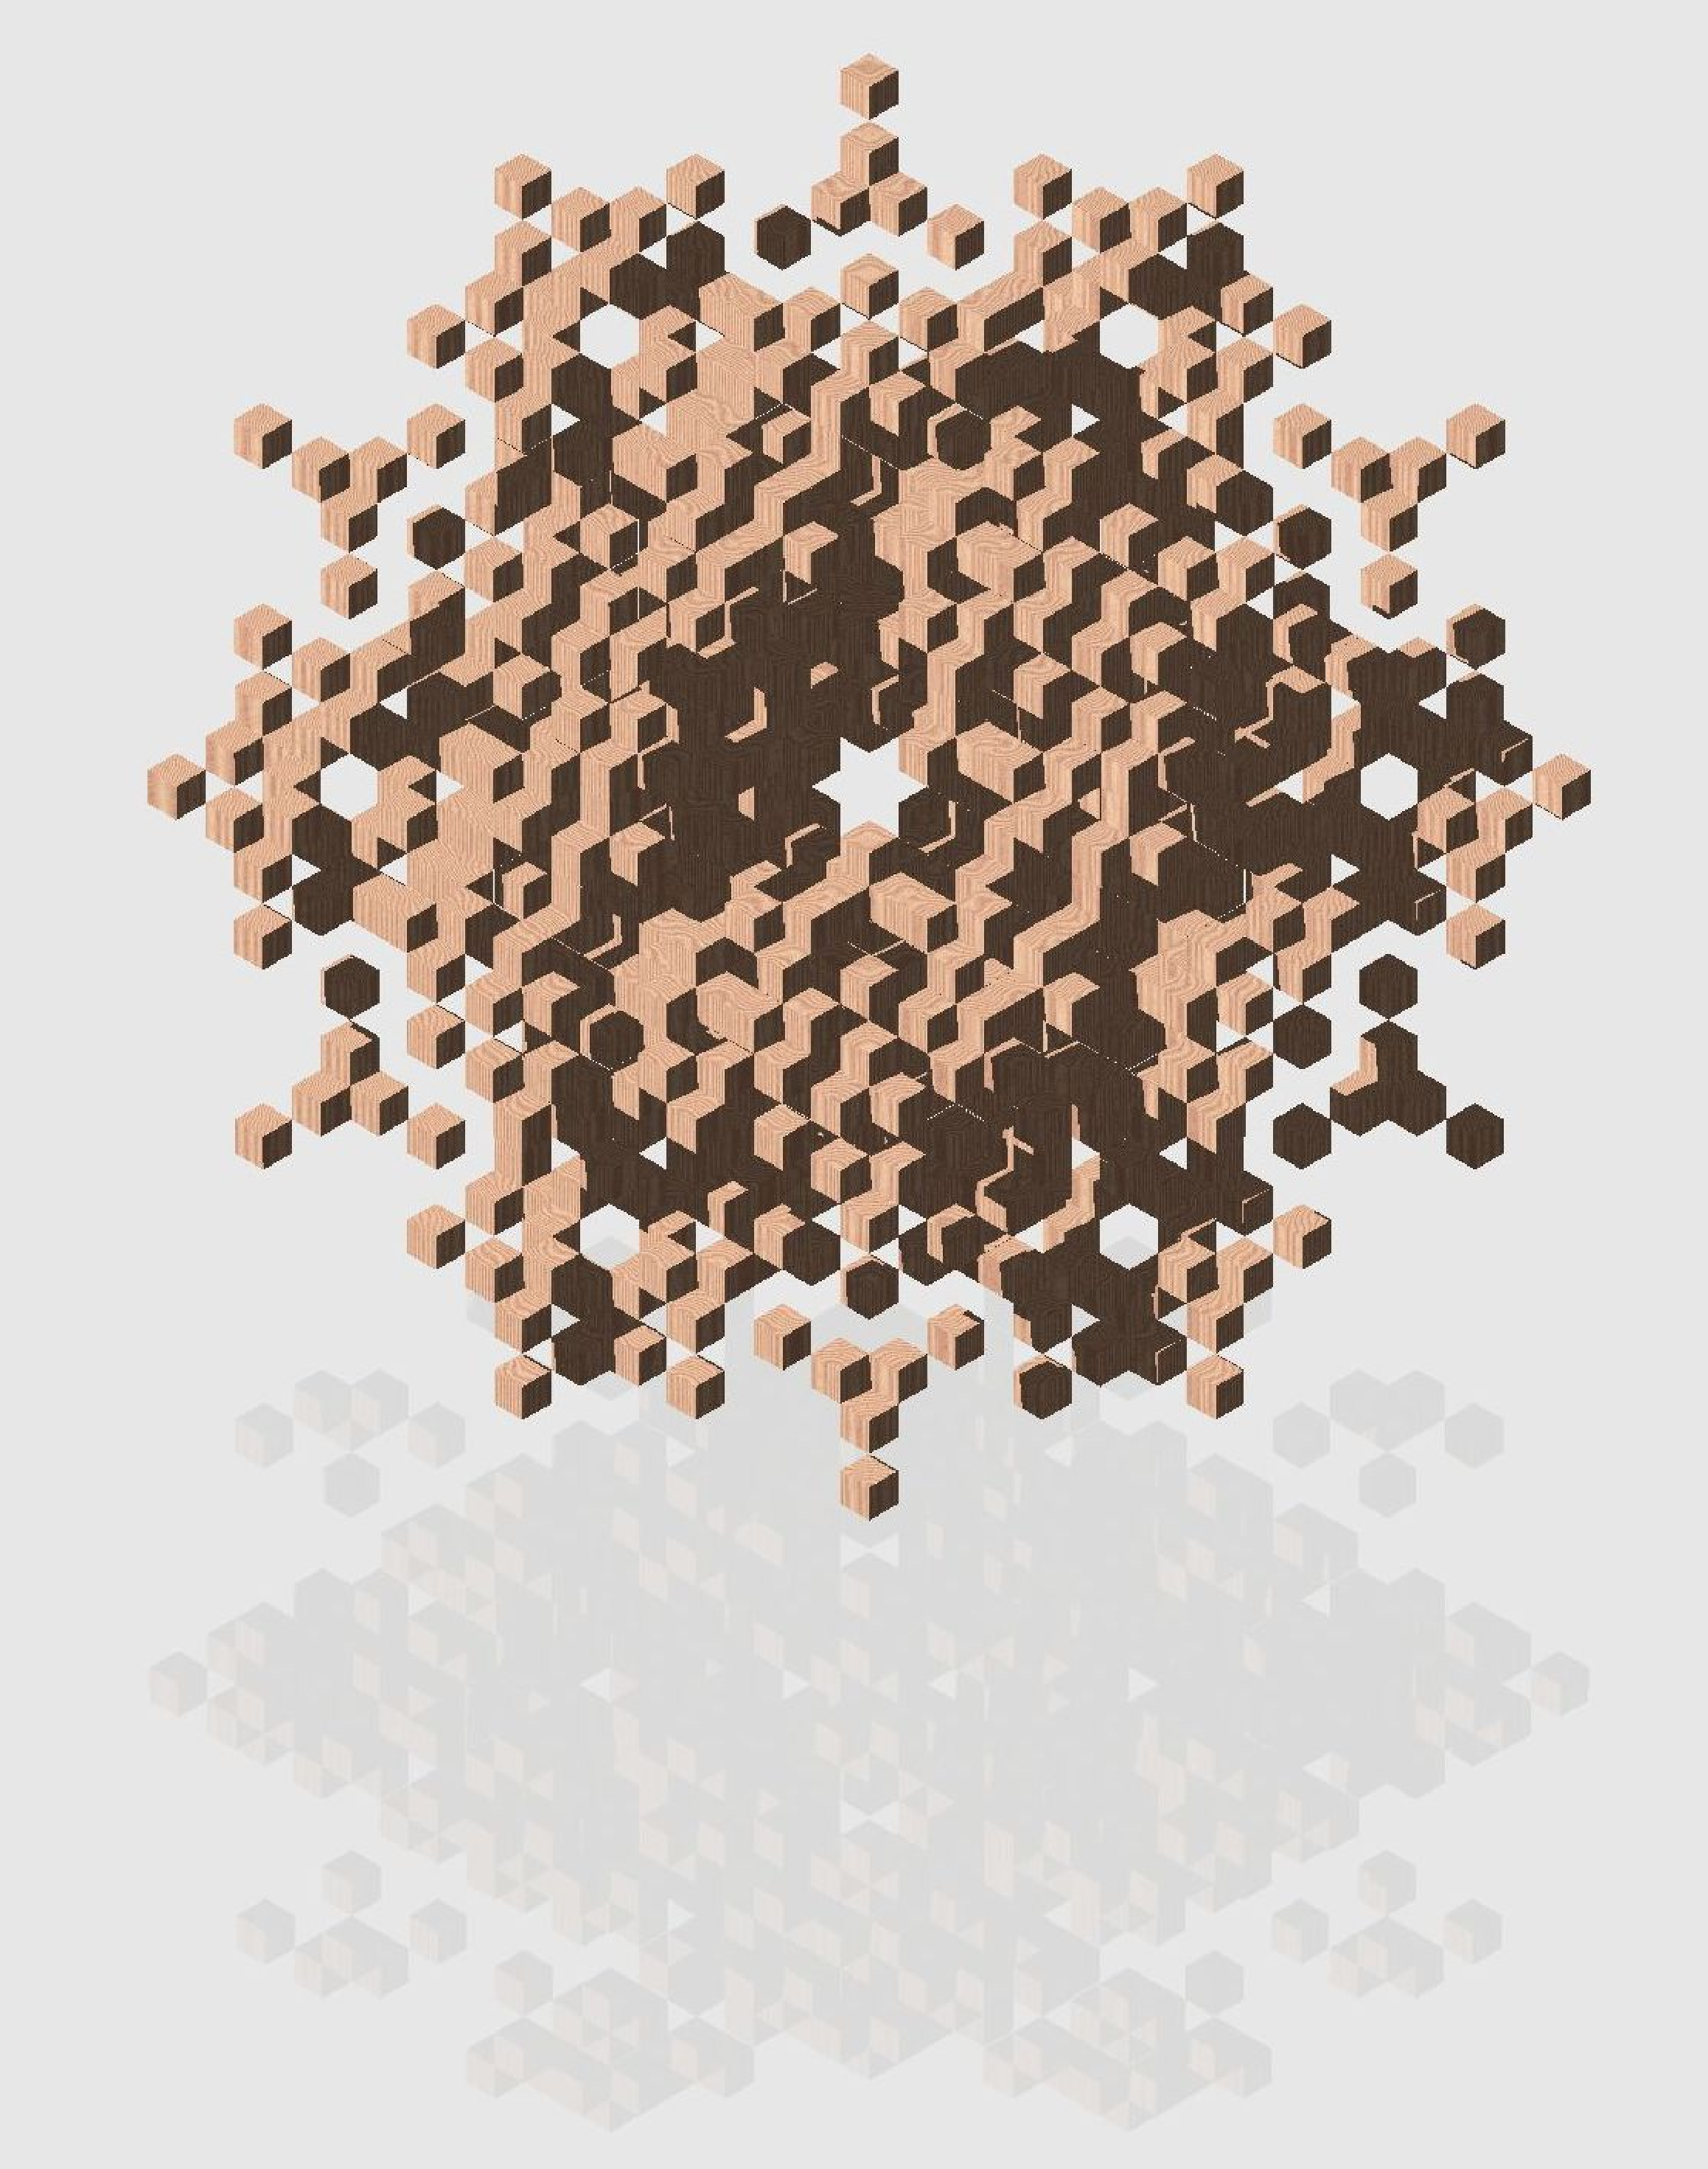
\includegraphics[width=2cm]{ccourse-logo.pdf}}



% Article version layout settings

\mode<article>

\makeatletter
\def\@listI{\leftmargin\leftmargini
  \parsep 0pt
  \topsep 5\p@   \@plus3\p@ \@minus5\p@
  \itemsep0pt}
\let\@listi=\@listI


\setbeamertemplate{frametitle}{\paragraph*{\insertframetitle\
    \ \small\insertframesubtitle}\ \par
}
\setbeamertemplate{frame end}{%
  \marginpar{\scriptsize\hbox to 1cm{\sffamily%
      \hfill\strut\insertshortlecture.\insertframenumber}\hrule height .2pt}}
\setlength{\marginparwidth}{1cm}
\setlength{\marginparsep}{4.5cm}

\def\@maketitle{\makechapter}

\def\makechapter{
  \newpage
  \null
  \vskip 2em%
  {%
    \parindent=0pt
    \raggedright
    \sffamily
    \vskip8pt
    {\fontsize{36pt}{36pt}\selectfont Kapitel \insertshortlecture \par\vskip2pt}
    {\fontsize{24pt}{28pt}\selectfont \color{blue!50!black} \insertlecture\par\vskip4pt}
    {\Large\selectfont \color{blue!50!black} \insertsubtitle\par}
    \vskip10pt

    \normalsize\selectfont Druckfassung der
    %\emph{\lecturename} vom \@date\par\vskip1.5em
    \@date\par\vskip1.5em
    %\hfill with thanks to Till Tantau, Institut f�r Theoretische Informatik, Universit�t zu L�beck
    \hfill Eidon (Eidon at tutanota.com)
  }
  \par
  \vskip 1.5em%
}

\let\origstartsection=\@startsection
\def\@startsection#1#2#3#4#5#6{%
  \origstartsection{#1}{#2}{#3}{#4}{#5}{#6\normalfont\sffamily\color{blue!50!black}\selectfont}}

\makeatother

\mode
<all>




% Typesetting Listings

\usepackage{listings}
\lstset{language=Java}

\alt<presentation>
{\lstset{%
  basicstyle=\footnotesize\ttfamily,
  commentstyle=\slshape\color{green!50!black},
  keywordstyle=\bfseries\color{blue!50!black},
  identifierstyle=\color{blue},
  stringstyle=\color{orange},
  escapechar=\#,
  emphstyle=\color{red}}
}
{
  \lstset{%
    basicstyle=\ttfamily,
    keywordstyle=\bfseries,
    commentstyle=\itshape,
    escapechar=\#,
    emphstyle=\bfseries\color{red}
  }
}



% Common theorem-like environments

\theoremstyle{definition}
\newtheorem{exercise}[theorem]{\translate{Exercise}}




% New useful definitions:

\newbox\mytempbox
\newdimen\mytempdimen

\newcommand\includegraphicscopyright[3][]{%
  \leavevmode\vbox{\vskip3pt\raggedright\setbox\mytempbox=\hbox{\includegraphics[#1]{#2}}%
    \mytempdimen=\wd\mytempbox\box\mytempbox\par\vskip1pt%
    \fontsize{3}{3.5}\selectfont{\color{black!25}{\vbox{\hsize=\mytempdimen#3}}}\vskip3pt%
}}

\newenvironment{colortabular}[1]{\medskip\rowcolors[]{1}{blue!20}{blue!10}\tabular{#1}\rowcolor{blue!40}}{\endtabular\medskip}

\def\equad{\leavevmode\hbox{}\quad}

\newenvironment{greencolortabular}[1]
{\medskip\rowcolors[]{1}{green!50!black!20}{green!50!black!10}%
  \tabular{#1}\rowcolor{green!50!black!40}}%
{\endtabular\medskip}





%\lecture[1]{A Short Course on\\C Language Programming}{lecture-text}
\lecture{C Language Programming}{A Short Course on C Language Programming}

\subtitle{A short course about C (actually about Lex and YACC too \Smiley)}

\date{27 June 2018}


\begin{document}

\begin{frame}
  \maketitle
\end{frame}

%\input{beamerexample-lecture-body.tex}
%%%%%%%%%%%%%%%%%%%%%%%%%%%%%%%%%%%%%%%%%%%%%%%%%%%%%%%%%%%%%%%%%%%%
\begin{frame}[fragile]{A Short Course on C Language Programming}
\begin{itemize}
\item \href{mailto:Eidon@tutanota.com}{Eidon@tutanota.com}
\item Course slides at \url{https://github.com/Eidonko/ccourse}
\item Course software at 
\url{https://github.com/Eidonko}
\end{itemize}
\end{frame}

\begin{frame}[fragile]{Objectives}
Provide the audience with a set of
\begin{itemize}
\item ideas,
\item methods,
\item and know-how
resulting from several years of design and development
with the C language in an engineering environment.

\item Problem solving with C: syntactical analysis.
\end{itemize}

\end{frame}
\begin{frame}[fragile]{Purpose and structure}
\begin{itemize}
\item An introduction to C
\item The \texttt{FILE} methodology. Classes. Data hiding.
      Examples (class assoc, objalloc, vf\ldots)
\item Literate programming. The cweb tools
\item The GNU Autotools
\item Other classes for embedded systems (class tom, the ``art'' framework)
\item Linguistic support using C, Lex and YACC.
      Examples (the icgi interpreter, class FN, PvmLinda,
      the Ariel language...)
\item Exercise sessions, case studies, project works
\end{itemize}

%%The daily structure is on the net.
%%%%%%%%%%%%%%%%%%%%%%%%%%%%%%%%%%%%%%%%%%%%%%%%%%%%%%%%%%%%%%


%%%%%%%%%%%%%%%%%%%%%%%%%%%%%%%%%%%%%%%%%%%%%%%%%%%%%%%%%%%%%%
\end{frame}
\begin{frame}[fragile]{Advanced C Language for Engineering}

Exam: a project work (coding plus documentation) to be 
sent to me by the end of the year.

\vspace*{1cm}

%%%%%%%%%%%%%%%%%%%%%%%%%%%%%%%%%%%%%%%%%%%%%%%%%%%%%%%%%%%%%%

\end{frame}
\begin{frame}[fragile]{``The'' problem}
Teaching C to an audience with different backgrounds and
different expectations is very difficult.


\vspace{20pt}

Tuning the course is difficult.


\vspace{20pt}

Exercise sessions are particularly problematic.
\end{frame}

\begin{frame}[fragile]{Solutions}
Ideally, the course should be \emph{ad personam}.
Strong interaction with the teacher is
suggested. Just \href{mailto:Eidon@tutanota.be}{mail me} with your questions.


\vspace{20pt}

Practically speaking, exercises will be organized in 2 levels:
for those with no practical experience vs. for those with
practical experience.

\begin{itemize}
\item level A : for instance, learning how to log in a UNIX
	system, how to edit a C program, how to compile, and execute it
\item level B : designing ``improved'' versions, e.g., code optimisations;
writing test programs using the C classes at
\url{https://github.com/Eidonko}, and so forth.
\end{itemize}


\vspace{20pt}

For experienced people,
exercise sessions can be devoted to the design of the
solution of the project works.
\end{frame}

\begin{frame}[fragile]{Introduction to C: Structure}
\begin{itemize}
\item Introduction 
\item First examples
\item Fundamental data types, derived data types
\item Derived types: pointers and vectors
\item Functions
\item Structures and unions
\item Data hiding
\end{itemize}
%%}}}
\end{frame}

%%{{{  Introduction
%%%%%%%%%%%%%%%%%%%%%%%%%%%%%%%%%%%%%%%%%%%%%%%%%%%%%%%

\begin{frame}[fragile]{Introduction to C}
\begin{itemize}
\item C and UNIX : success stories.
\item C: developed by Ritchie to port UNIX from a PDP-7 to a PDP-11
\item System programming language
\item Most of the UNIX system is in C
\end{itemize}

%%%%%%%%%%%%%%%%%%%%%%%%%%%%%%%%%%%%%%%%%%%%%%%%%%%%%%%
\end{frame}
\begin{frame}[fragile]{Introduction to C}
\begin{itemize}
\item C is simple:
  \begin{itemize}
  \item A small number of simple and powerful instructions
  \item dealing with characters, numbers, addresses
  \item No language facilities for handling complex objects
        (strings, lists...)
  \item No language facilities for the I/O, for memory allocation...
  \end{itemize}
\item Those facilities are available as standard (or user-defined)
      libraries of functions
\end{itemize}
%%%%%%%%%%%%%%%%%%%%%%%%%%%%%%%%%%%%%%%%%%%%%%%%%%%%%%%
\end{frame}

\begin{frame}[fragile]{Introduction to C}
\begin{itemize}
\item C is small:
  \begin{itemize}
  \item Easy to describe, easy to learn
  \item The C compiler is considerably simple, compact-sized,
        and easy to write
\item The C data types and control structures often have
      a direct equivalent in the machine language of many
      computers. This happens because C was modelled after
      the machine language of the PDP 11. 
\item Hence, while in general the translation from a
      high level language instruction to machine language 
      is in general one-to-many, the translation from C
      to machine language is \textbf{one-to-few}.
\item A very simple run-time system: for instance (PDP-11)
         \index{PDP-11}:
   \begin{itemize}\item routines for 32-bit or 64-bit {\tt *} and {\tt /}.
      \item management of subroutine entry and exit.\end{itemize}
   \end{itemize}
\end{itemize}
\end{frame}
%%%%%%%%%%%%%%%%%%%%%%%%%%%%%%%%%%%%%%%%%%%%%%%%%%%%%%%

\begin{frame}[fragile]{Introduction to C}
C is portable\ldots

  \begin{itemize}
  \item but we need to follow some portability rules
  \item types have no well-defined size (e.g., in Python we have 
  	\texttt{numpy.int32}, in C we don't have an a-priori knowledge
	of the size of an \texttt{int})
  \item we can use symbolic constants for this
  \item large set of standard libraries for I/O, string manipulation,
  	memory allocation\ldots
  \end{itemize}

\end{frame}

%%%%%%%%%%%%%%%%%%%%%%%%%%%%%%%%%%%%%%%%%%%%%%%%%%%%%%%

\begin{frame}[fragile]{Introduction to C}
\parbox{1.0in}{BCPL\index{BCPL} \\ (typeless language\\by M. Richards)} $\Rightarrow$
\parbox{1.0in}{B Language\index{B Language} \\ (typeless lang.\\
 by K.  Thompson)} $\Rightarrow$
\parbox{1.0in}{C Language\\ (non-typeless,
 non-strongly-typed\index{Strongly-Typed Languages}
 language) by D. M.~Ritchie}

 \begin{description}
 \item[Typeless Language]: data are organized as multiple instances of the machine word.
 	Everything is allowed. Example: Assembly
 \item[Strongly-Typed\index{Strongly-Typed Languages} Language]: Nearly every
 	cast from type
 $A$ to type $B$ needs to be explicitly requested. Once a variable of a given type
 has been defined, also its
 {\em run-time checking\/} is defined in order to detect, e.g., overflow, underflow,
 subscript-out-of-range conditions, and so forth.
 ecc.  Examples: Pascal\index{Pascal}, Ada\index{Ada}.
 \end{description}


%%%%%%%%%%%%%%%%%%%%%%%%%%%%%%%%%%%%%%%%%%%%%%%%%%%%%%%
\end{frame}
\begin{frame}[fragile]{Introduction to C}
C is not a typeless language\index{Typeless Languages}: basic types are available
\begin{itemize}\item characters\item integers (in various sizes)
\item floating point numbers (in different sizes)
\item pointers\item facilities to build complex types from the basic types:
arrays\index{array}, records,
``unions\index{\tt union}'', functions.
\end{itemize}


\vspace{20pt}

C is not a strongly-typed\index{Strongly-Typed Languages} language:
it is {\em permissive\/}
about data casts. Its run-time executive does not cover
run-time checking.


%%%%%%%%%%%%%%%%%%%%%%%%%%%%%%%%%%%%%%%%%%%%%%%%%%%%%%%
\end{frame}
\begin{frame}[fragile]{Introduction to C}
C provides:
\begin{itemize}
\item the basic control-flow statements
    \begin{itemize} \item statement grouping
                    \item selective statements
                    \item iterative statements
    \end{itemize}
\item pointers\index{pointers} + {\em address arithmetic}
\end{itemize}

%%%%%%%%%%%%%%%%%%%%%%%%%%%%%%%%%%%%%%%%%%%%%%%%%%%%%%%
\end{frame}
\begin{frame}[fragile]{Introduction to C: Functions}
\begin{itemize}
\item Note:
     \begin{itemize}\item only call-by-value
                    \item recursion is allowed
                    \item single-level functions
                      that can be compiled separately.
                    \item variables
                      \begin{itemize} \item scope:
                                        ``blo\-ck-stru\-ctu\-red fashion''
			\item static vs. automatic
                      \end{itemize}
     \end{itemize}
\end{itemize}


%%%%%%%%%%%%%%%%%%%%%%%%%%%%%%%%%%%%%%%%%%%%%%%%%%%%%%%
\end{frame}
\begin{frame}[fragile]{Introduction to C}
\begin{verse}
 ``The only way to learn a new programming language is by writing
   programs in it; the first program to write is the same for all
   languages: print the words \texttt{"hello, world"}.'' [KR]

 ``What we have to learn to do we learn by doing.'' [Aristotle]
\end{verse}


\vspace{20pt}

\begin{verbatim}
           main()    /* prints "hello world." */
           {         /* and goes to the next line */
               printf("hello world.\n");
           }
\end{verbatim}

%%%%%%%%%%%%%%%%%%%%%%%%%%%%%%%%%%%%%%%%%%%%%%%%%%%%%%%
\end{frame}

\begin{frame}[fragile]{Introduction to C}
\begin{itemize}
\item Log into your Linux workstation\index{Linux}
\item type the {\tt "hello, world"} program
\item compile it
\item execute it
\end{itemize}



%%%%%%%%%%%%%%%%%%%%%%%%%%%%%%%%%%%%%%%%%%%%%%%%%%%%%%%
\end{frame}
\begin{frame}[fragile]{Introduction to C: a classic example}
\begin{verbatim}
/* The famous Fahrenheit to Celsius conversion :-) */
/* From the KC book! */
void main() {
    int inf, sup, step;
    float fahr, celsius;

    inf = 0;
    sup = 300;
    step = 20;

    fahr = inf;
    while  (fahr <= sup)  {
           celsius = (5.0/9.0) * (fahr-32.0);
           printf("%4.0f %6.1f\n", fahr, celsius);
           fahr = fahr + step;
    }
}
\end{verbatim}


%%%%%%%%%%%%%%%%%%%%%%%%%%%%%%%%%%%%%%%%%%%%%%%%%%%%%%%
\end{frame}
\begin{frame}[fragile]{Introduction to C}

Adapt the above code so to do the opposite
conversion.


\vspace{20pt}

Try to answer the following questions:
\begin{itemize}
\item why \verb"5.0/9.0" and not \verb"5/9"?
\item is \verb"5.0/9" equivalent to \verb"5.0/9.0"?
\item is the \verb".0" really necessary in \verb"fahr-32.0"?
\end{itemize}


%%%%%%%%%%%%%%%%%%%%%%%%%%%%%%%%%%%%%%%%%%%%%%%%%%%%%%%
\end{frame}
\begin{frame}[fragile]{Introduction to C: while loops}
\begin{verbatim}
while ( test ) action
\end{verbatim}


\vspace{20pt}

\verb"test" is executed. If output is non-zero (``true'') then
 \verb"action" is executed.

\vspace{20pt}


\verb"action" can also be a composite action
using curly brackets.


\vspace{20pt}

\begin{verbatim}
for (init; test; incr) action
\end{verbatim}

\noindent
is equivalent to
\begin{verbatim}
  init;
  while (test) { action; incr; }
\end{verbatim}


%%%%%%%%%%%%%%%%%%%%%%%%%%%%%%%%%%%%%%%%%%%%%%%%%%%%%%%
\end{frame}
\begin{frame}[fragile]{Introduction to C}

\verb"init", \verb"test", \verb"incr", and \verb"action" are all optional arguments: even
\begin{center}\tt for (;;) ;\end{center}
is allowed.

\vspace{20pt}

Note: \verb"test" is a {\em statement\/}!

\vspace{20pt}

Both {\tt while (a=3) ...} and {\tt while (a==3) ...} are valid!



%%%%%%%%%%%%%%%%%%%%%%%%%%%%%%%%%%%%%%%%%%%%%%%%%%%%%%%
\end{frame}
\begin{frame}[fragile]{Introduction to C}
Exercise: modify the previous example so to change the \verb"while" into \verb"for".

\vspace{20pt}

Exercise:  modify the previous example so to print the table in inverse order.


%%%%%%%%%%%%%%%%%%%%%%%%%%%%%%%%%%%%%%%%%%%%%%%%%%%%%%%
\end{frame}
\begin{frame}[fragile]{Introduction to C: conditional statements}
\begin{itemize}
\item statement ``if'':     \\
      if (condition) action${}_1$; else action${}_2$; \\
      (nesting and so forth.)
\item ``?:'' \\
      (condition)? action${}_1$ : action${}_2$;
\item ``switch'': \\
      switch(integer\_expr) \{  \\
      case value${}_1$: op${}_1$; break; \\
      case value${}_2$: op${}_2$; break; \\
      $\vdots$ \\
      case value${}_n$: op${}_n$; break; \\
      default: op${}_{n+1}$; \}
\end{itemize}


%%%%%%%%%%%%%%%%%%%%%%%%%%%%%%%%%%%%%%%%%%%%%%%%%%%%%%%
\end{frame}
\begin{frame}[fragile]{Introduction to C: loops and related statements}
\begin{itemize}
\item for
\item while
\item do while
\item break;
\item continue;
\item goto label
\end{itemize}


%%%%%%%%%%%%%%%%%%%%%%%%%%%%%%%%%%%%%%%%%%%%%%%%%%%%%%%
\end{frame}
\begin{frame}[fragile]{Introduction to C: defines and includes}
In C, it is possible to define symbolic constants via the \verb"#define"
pre-processor directive, and to specify that an external file should
be read in at compile time, via the \verb"#include"
pre-processor directive.


\vspace{20pt}

A few examples follow:

\begin{tabular}{||lll||} \hline\hline
\#define\index{\#DEFINE} & BEGIN & \{  \\
\#define & END   & \}  \\
\#define & IF    & if( \\
\#define & THEN  & ) \\
\#define & INT32 & long \\
\#define & INT32 & int \\
\#include & {\tt "file"} & \\
\#include & {\tt $<$file$>$} & \\ \hline\hline
\end{tabular}



%%%%%%%%%%%%%%%%%%%%%%%%%%%%%%%%%%%%%%%%%%%%%%%%%%%%%%%
\end{frame}
\begin{frame}[fragile]{Introduction to C: other pre-processor directives}
\begin{itemize}
\item macro substitution (e.g., {\tt \#define TRUE 1})
\item macro with parameters: \\
   \#define $MAX(a,b)\ \ ((A)>(B)$ ? $(A):(B))$ \\
   (Note: \#define sqr$(x)=$ $x*x$ is error-prone. Can you tell why?)
\item Conditional inclusion: ({\tt \#ifdef} and {\tt \#ifndef},
{\tt \#else} and {\tt \#endif}.)
\end{itemize}


%%%%%%%%%%%%%%%%%%%%%%%%%%%%%%%%%%%%%%%%%%%%%%%%%%%%%%%
\end{frame}
\begin{frame}[fragile]{Introduction to C: first functions for standard I/O}
\begin{itemize}
\item Defined in $<$stdio.h$>$
\item getchar (e.g. c=getchar()\index{I/O}), putchar (e.g. putchar(c)),
\EOF...
\end{itemize}


\vspace{20pt}

Example: copy of input to output --- version 1.


\vspace{20pt}

\begin{tt}
\begin{verbatim}
    #include <stdio.h>
    int main() { int c;
     c=getchar();
     while (c != EOF ) {
         putchar (c);
         c=getchar();
     }
    }
\end{verbatim}
\end{tt}



%%%%%%%%%%%%%%%%%%%%%%%%%%%%%%%%%%%%%%%%%%%%%%%%%%%%%%%
\end{frame}
\begin{frame}[fragile]{Introduction to C: first functions for standard I/O}
Example: copy of input to output --- version 2.


\vspace{20pt}

\begin{tt}
\begin{verbatim}
    #include <stdio.h>
    main() { int c;

    while ((c = getchar()) != EOF )
        putchar (c);
    }
\end{verbatim}
\end{tt}


\vspace{20pt}

Note: parentheses around \verb"c = getchar()" are necessary, because
of the larger priority of \verb"!=" with respect to \verb"=".



%%%%%%%%%%%%%%%%%%%%%%%%%%%%%%%%%%%%%%%%%%%%%%%%%%%%%%%
\end{frame}
\begin{frame}[fragile]{Introduction to C: first functions for standard I/O}
Exercise:
the just seen program can be easily adapted to work, e.g.,
as a ``word counter'' (reports the number of characters,
words, and lines in the input), or as a filter to remove blanks or
tabs, and so forth.


\vspace{20pt}

Input and output can be redirected with \verb"<" and \verb">".
Pipelines of programs can be built by chaining the programs with \verb"|".


%%%%%%%%%%%%%%%%%%%%%%%%%%%%%%%%%%%%%%%%%%%%%%%%%%%%%%%
\end{frame}
\begin{frame}[fragile]{Introduction to C: arrays}

To declare an array in C one has to use the following
syntax:

\vspace{20pt}

\begin{center}type name [dimension1][dimension2]..[dimension${}_n$] ;
\end{center} 


\vspace{20pt}

For instance, {\tt int vect[10];}


\vspace{20pt}

This is equivalent to e.g.
{\tt vect = numpy.array(10, dtype=numpy.int)}
in Python.


\vspace{20pt}


The index can be any integer expression.
  

\vspace{20pt}

There is no bound check like, e.g., in Ada.


%%%%%%%%%%%%%%%%%%%%%%%%%%%%%%%%%%%%%%%%%%%%%%%%%%%%%%%
\end{frame}
\begin{frame}[fragile]{Introduction to C: arrays}
Note: declaring an array means
\begin{enumerate}
\item declaring a \textbf{pointer}
\item and allocating memory for the pointed objects.
\end{enumerate}
The name of the array is indeed a pointer to the first element of the
array. In C lingo, this is written as
{\tt vect == \&vect[0]}. \label{arrayref}


\vspace{20pt}

Esercise: write a program, called report, that reports the occurrences of
each digit char in the input stream. Use an array of ten elements corresponding
to the ten decimal digits. Produce an histogram at end-of-input.

%%%%%%%%%%%%%%%%%%%%%%%%%%%%%%%%%%%%%%%%%%%%%%%%%%%%%%%
\end{frame}
\begin{frame}[fragile]{Introduction to C: arrays}
Exercise: use two programs, one that outputs the ten integer numbers
that count the occurrences of
each digit char in the input stream, the other one that creates a histogram
of its input values. Then use a pipeline to hook the two programs together.


\vspace{20pt}

\begin{center}
{\tt report2  |  histogram}
\end{center}



%%%%%%%%%%%%%%%%%%%%%%%%%%%%%%%%%%%%%%%%%%%%%%%%%%%%%%%
\end{frame}
\begin{frame}[fragile]{Introduction to C: functions}

Functions are named fragments of C code that can accept arguments and
return a value of some type.


\vspace{20pt}

Functions are, e.g., printf(), getchar()\index{I/O}, putchar(), main()\ldots\


\vspace{20pt}

No function hierarchy is allowed. The only ``special'' function is
main(). Functions can reside in a same source file or in more than one.



%%%%%%%%%%%%%%%%%%%%%%%%%%%%%%%%%%%%%%%%%%%%%%%%%%%%%%%
\end{frame}
\begin{frame}[fragile]{Introduction to C: functions}
Functions have the following structure: 


\vspace{20pt}

   {\tt [type]} {\em name\/} {\tt ( [ {\em args\/} ] ) }


   {\tt \{ [ {\em declarations\/} ] [ {\em instructions\/} ] \} }


\vspace{20pt}

\begin{tt}
\begin{verbatim}
  int main() {
      int i; int power (int, int);
      for (i=0; i<10; ++i)
          printf("%d %d\n", i, power(2,i));
  }
  int power (int x, int n) { int i, p;
    for (i = p = 1; i <= n; ++i)
       p=p*x;
    return (p);
  }
\end{verbatim}
\end{tt}
%%%%%%%%%%%%%%%%%%%%%%%%%%%%%%%%%%%%%%%%%%%%%%%%%%%%%%%
\end{frame}

\begin{frame}[fragile]{Introduction to C}

\texttt{return} closes the function and returns an output value
(default: integer) to the caller.


\vspace{20pt}

Arguments are passed \textbf{by value}: this means that
the arguments are copied in temporary variables.


\vspace{20pt}

The only way to let a function modify an argument is by passing
\emph{the address\/} of the object to be modified. 


\vspace{20pt}

Operator \verb"&" returns the address of a variable.


\vspace{20pt}

Note that, when you need to pass an array, passing its name is
indeed passing a pointer to the array.


%%%%%%%%%%%%%%%%%%%%%%%%%%%%%%%%%%%%%%%%%%%%%%%%%%%%%%%
\end{frame}
\begin{frame}[fragile]{Introduction to C: strings}
Strings are available in C as arrays of characters. Any sentence
enclosed between two \verb'"''s is an array of characters ending
with character \verb"'\0'" (NULL).


\vspace{20pt}

For instance, {\tt "hello"} $\Rightarrow$ 'h', 'e', 'l', 'l', 'o', 0


\vspace{20pt}

A very common mistake when learning C:

\begin{tt}
\begin{verbatim}
  char s1[10] = "Hello ";
  char s2[10] = "World";

  s1=s2;    /* ERROR */
\end{verbatim}
\end{tt}



%%%%%%%%%%%%%%%%%%%%%%%%%%%%%%%%%%%%%%%%%%%%%%%%%%%%%%%
\end{frame}
\begin{frame}[fragile]{Introduction to C}
As strings are arrays, we can easily pass a string to a function
by passing its name, which points to its characters:


\vspace{20pt}

\begin{verbatim}
  char a[] = "Pogo Possum";
  printf("Vote %s for president.\n", a);
  /* a = &a[0] */
\end{verbatim}


Variables defined within a function cannot be ``seen'' from other functions.

\vspace{20pt}


Two main classes of variables: {\tt automatic} vs. {\tt static}. Automatic variables
are allocated at function call and deallocated when the function stops.
They require initialisation. Static variables are allocated at compile time.
They are initialised to zero, and \emph{keep the value we left in them
when we get out of the functions where they are defined.}


%%%%%%%%%%%%%%%%%%%%%%%%%%%%%%%%%%%%%%%%%%%%%%%%%%%%%%%
\end{frame}
\begin{frame}[fragile]{Introduction to C}
\begin{itemize}
\item identifiers have the following structure:
      $<$alpha$>$ { $<$alphanum$>$ }*
\item six basic types: char, short, int, long, float, double.
\item qualifiers: unsigned, register
\item constants:
    \begin{itemize}
    \item scientific notation, e.g., {\tt 1.5e3} $\rightarrow$ double
    \item postfix notation, e.g., 145L $\rightarrow$ long
    \item prefix notation: '0x44' $\rightarrow$ unsigned int, hexadecimal, '044'
          $\rightarrow$ unsigned int, octal
    \item costant char. \verb"'c'" = character c  $\rightarrow$ char
\end{itemize}
\end{itemize}

%%%%%%%%%%%%%%%%%%%%%%%%%%%%%%%%%%%%%%%%%%%%%%%%%%%%%%%
\end{frame}
\begin{frame}[fragile]{Introduction to C}
    \begin{itemize}
    \item special constants, e.g., \verb"\n", \verb"\t", \verb"\0", \verb"\\", \verb'\"' and so forth  $\rightarrow$ char
    \item ``bit patterns'': \verb"\ddd", \verb"ddd" being an octal number.
    \item string constants, e.g., {\tt "string"} or {\tt ""}.
\end{itemize}


\vspace{20pt}

Exercise: write a function that counts the number of character
pointed by its string argument ({\tt strlen}).



%%%%%%%%%%%%%%%%%%%%%%%%%%%%%%%%%%%%%%%%%%%%%%%%%%%%%%%
\end{frame}
\begin{frame}[fragile]{Introduction to C: declarative instructions}
\begin{itemize}
\item Declarative instructions take the following form: \\
	\emph{typename list-of-variables;}
\item A declarative instruction can be followed
by an initialisation: \\
	int n=5; float g=5.4;
\item If the variable is an automatic one, then the initialisation is done
      \emph{each time the variable is allocated\/} (each time the function in which
      the variable resides is called).
\end{itemize}

%%%%%%%%%%%%%%%%%%%%%%%%%%%%%%%%%%%%%%%%%%%%%%%%%%%%%%%
\end{frame}
\begin{frame}[fragile]{Introduction to C: declarative instructions}
\begin{itemize}
\item Non-initialised automatic variables contain random value.
\item If the variable is a static one, then the initialisation is done
\emph{only once\/} (at compile time).
\item Static variables are always initialised. Default=0.
\item \emph{Global, static variables are only visible to the functions
      in the same source file}: this can be used for data hiding.
\end{itemize}



%%%%%%%%%%%%%%%%%%%%%%%%%%%%%%%%%%%%%%%%%%%%%%%%%%%%%%%
\end{frame}
\begin{frame}[fragile]{Introduction to C: operators}
\begin{itemize}
\item binary: +, -, $\ast$, /, \%
\item unary {\bf -}
\item precedences\index{precedenza}: +,- $<_{\rm prec}$ $\ast$,/,\% $<_{\rm prec}$ {\bf -}
\end{itemize}


\vspace{20pt}

\begin{itemize}
\item {\tt ||} \pre
\item \&\& \pre
\item == and !=, \pre
\item $>$ $>=$ $<$ $<=$
\end{itemize}


%%%%%%%%%%%%%%%%%%%%%%%%%%%%%%%%%%%%%%%%%%%%%%%%%%%%%%%
\end{frame}
\begin{frame}[fragile]{Introduction to C: operators}
Expressions such as:

\vspace{20pt}

\begin{center}
$i<lim$ \&\& (c=getchar()\index{I/O}) != '\\n' \&\& c != \EOF
\end{center}
do not require extra parentheses:
 =\pre !=, hence parentheses are required around
\verb"c=getchar()".


\vspace{20pt}

Logic clauses are evaluated left-to-right. Evaluation stops when the truth value
of a logic expression is ascertained.



%%%%%%%%%%%%%%%%%%%%%%%%%%%%%%%%%%%%%%%%%%%%%%%%%%%%%%%
\end{frame}
\begin{frame}[fragile]{Introduction to C: derived types}

The following operators define complex types derived from the
basic types of C:

\vspace{20pt}

\begin{description}
\item[\texttt{*}] operator pointer-to,
\item[\texttt{[]}] operator vector-of,
\item[\texttt{()}] operator pointer-to-function.
\end{description}

%%%%%%%%%%%%%%%%%%%%%%%%%%%%%%%%%%%%%%%%%%%%%%%%%%%%%%%
\end{frame}
\begin{frame}[fragile]{Introduction to C: derived types}
\begin{itemize}
\item \verb"char *p;" : \verb"p" is of type ``pointer-to-chars''
\item \verb"float v[10];" : \verb"v" is a vector, i.e., a pointer to the beginning of
  a memory area allocated by the system and consisting of 10 floats, i.e.,
  \verb"v[0]", \ldots, \verb"v[9]".
\item \verb"int getX();" : \verb"getX" is a pointer to a function returning an int.
\end{itemize}


%%%%%%%%%%%%%%%%%%%%%%%%%%%%%%%%%%%%%%%%%%%%%%%%%%%%%%%
\end{frame}
\begin{frame}[fragile]{Introduction to C: derived types}
Operator \verb"[]" has higher priority with respect to operator
\verb"*". This means that


\vspace{20pt}

\begin{center}
           \tt int *v[10]
\end{center}


\vspace{20pt}

\noindent means that \verb"v" is a vector of ten pointers-to-int.
Parentheses are necessary to change the meaning:


\vspace{20pt}

\begin{center}
           \tt int (*v)[10]
\end{center}

\noindent means that \verb"v" is a pointer to a vector of ten integers.


\vspace{20pt}

What's the difference in terms of sizes?


%%%%%%%%%%%%%%%%%%%%%%%%%%%%%%%%%%%%%%%%%%%%%%%%%%%%%%%
\end{frame}
\begin{frame}[fragile]{Introduction to C: derived types}
%%%%%%%%%%%%%%%%%%%%%%%%%%%%%%%%%%%%%%%%%%%%%%%%%%%%%%%
\begin{enumerate}
\item \verb"int *pi;" : pointer to integer;
\item \verb"char **argv;" : pointer to pointer-to-char;
\item \verb"float *(fvp)[5];" : pointer to vectors-of-5-floats
\item \verb"long (*fp)(int);" : pointer to function reading an int and returning a long.
\end{enumerate}

%%%%%%%%%%%%%%%%%%%%%%%%%%%%%%%%%%%%%%%%%%%%%%%%%%%%%%%
\end{frame}
\begin{frame}[fragile]{Introduction to C: derived types}
%%%%%%%%%%%%%%%%%%%%%%%%%%%%%%%%%%%%%%%%%%%%%%%%%%%%%%%
The address-of (\verb"&") operator returns the address of a variable.


\vspace{20pt}

\begin{verbatim}
char c; char *pc;   pc = &pc;
\end{verbatim}


\vspace{20pt}

Operator \verb"*", applied to a pointer, returns the pointed object.


\vspace{20pt}

\begin{verbatim}
char c1 = 'a';   char *p = &c1;
char c2 = *p2;   /* c2 == 'a' */
\end{verbatim}


\vspace{20pt}

\begin{verbatim}
void func(char *s) { printf("bye %s\n", s) }

main() { void (*pfunc)(char*) = func;
         *(pfunc)("hello");
     }
\end{verbatim}

%%%%%%%%%%%%%%%%%%%%%%%%%%%%%%%%%%%%%%%%%%%%%%%%%%%%%%%
\end{frame}
\begin{frame}[fragile]{Introduction to C: derived types}
%%%%%%%%%%%%%%%%%%%%%%%%%%%%%%%%%%%%%%%%%%%%%%%%%%%%%%%
Pointers solve the problem of the lack of ``call-by-reference''
in C functions. For instance, in order to realize a function that
swaps its argument, one may use the following strategy:


\vspace{20pt}

\begin{verbatim}
 int swap(int *a, int *b) { int t;
     t = *a,   *a = *b,    *b = t;
 }
\end{verbatim}


\vspace{20pt}

The caller then needs to specify the addresses of the operands (s)he wants to
swap, as in \verb"swap(&i, &j)".


%%%%%%%%%%%%%%%%%%%%%%%%%%%%%%%%%%%%%%%%%%%%%%%%%%%%%%%
\end{frame}
\begin{frame}[fragile]{Introduction to C: derived types}
%%%%%%%%%%%%%%%%%%%%%%%%%%%%%%%%%%%%%%%%%%%%%%%%%%%%%%%
Arrays and pointers are strictly related to each other:
In particular, if {\tt int a[10];}
then a $\equiv$ \&a[0], a+1 $\equiv$ \&a[1] and so forth.
In other words,
\begin{center}\tt *(a+i) $\equiv$ a[i] \end{center}


\vspace{20pt}

Any indexed array is equivalent to
a pointer plus some offset, and vice-versa.


\vspace{20pt}

Big difference: the array is a constant, i.e., it can never 
appear on the left hand side of the \verb"=" sign, as in
$$a=pa$$
or in
$$a++$$

%%%%%%%%%%%%%%%%%%%%%%%%%%%%%%%%%%%%%%%%%%%%%%%%%%%%%%%
\end{frame}
\begin{frame}[fragile]{Introduction to C: derived types}
%%%%%%%%%%%%%%%%%%%%%%%%%%%%%%%%%%%%%%%%%%%%%%%%%%%%%%%
When passing an array to a function
we are indeed passing the address of its first element; this
address is copied 
(call-by-value) in a temporary variable. This variable may be
a pointer.


\vspace{20pt}

Example:

\begin{verbatim}
   char s[7] = "hello!";  /* s is an array */
   int  i = strlen(s);

   int strlen (char *x) { /* x is a pointer */
      int n;
      for (n=0; *x; x++)  /* hence, can be modified */
         n++;
      return (n);
   }
\end{verbatim}



%%%%%%%%%%%%%%%%%%%%%%%%%%%%%%%%%%%%%%%%%%%%%%%%%%%%%%%
\end{frame}
\begin{frame}[fragile]{Introduction to C: address arithmetics}
%%%%%%%%%%%%%%%%%%%%%%%%%%%%%%%%%%%%%%%%%%%%%%%%%%%%%%%
If p is a pointer, p++ lets p point to the next item.
It is the language that takes care of moving p of the
right amount of memory.


\vspace{20pt}

For instance,
\begin{tabular}{lll}
\multicolumn{3}{c}{\Int$\equiv$ 2 byte} \\
int *p;      &   \&p = 1222    & \&(p++) = 1224 \\
\multicolumn{3}{c}{\Double$\equiv$ 8 byte} \\
double *p;   &   \&p = 5644    & \&(p++) = 5660 \\
\multicolumn{3}{c}{and so forth}
\end{tabular}


\vspace{20pt}

In other words:
if p is a pointer to an object of type t, then
p+n points n objects further and p-n points n objects before.
The actual size of the object doesn't matter.




\end{frame}
\begin{frame}[fragile]{Introduction to C: type casts}
Implicit type casts occur when, in expressions, operands belong to different types.  Conversions obey the following rules:

\vspace{20pt}

\begin{itemize}
\item \Char and \Short $\rightarrow$ \Int, \Float $\rightarrow$ \Double
\item if an operand is \Double{}, the other becomes \Double and the result is
\Double
\item otherwise, if an operand is \Long, the other becomes \Long and the result is a
\Long
\item  otherwise, if an operand is unsigned, the other one becomes unsigned
and the result is unsigned.
\item otherwise, operands and result are \Int.
\end{itemize}


%%%%%%%%%%%%%%%%%%%%%%%%%%%%%%%%%%%%%%%%%%%%%%%%%%%%%%%
\end{frame}
\begin{frame}[fragile]{Introduction to C: conversions}
Converting a string of digits into a number, and vice-versa,
requires specific support.
Functions are available for this, e.g., \verb"atoi()":


\vspace{20pt}

\begin{tt}
\begin{verbatim}
   int atoi(char s[]) { int i, n;
        n = 0;
        for (i=0; s[i]>='0' && s[i]<='9'; ++i)
            n=10*n + s[i] -'0';
        return (n);
   }
\end{verbatim}
\end{tt}


\vspace{20pt}

Note how expression  {\tt s[i] - '0'} converts numeric character
\verb"s[i]" into the digit it represents.


%%%%%%%%%%%%%%%%%%%%%%%%%%%%%%%%%%%%%%%%%%%%%%%%%%%%%%%
\end{frame}
\begin{frame}[fragile]{Introduction to C: conversions}
The following function can be used to convert an uppercase character
into its lowercase counterpart.


\vspace{20pt}

\begin{tt}
\begin{verbatim}
      lower(c)
      int c;
      {
        if (c >='A' && c <= 'Z')
           return (c + 'a' - 'A');
        else
           return (c);
      }
\end{verbatim}
\end{tt}


\vspace{20pt}

Note: this program only works for code tables in which \verb"'a'"
follows \verb"'A'". This is true with ASCII and false with other codes
(e.g., EBCDIC.)


%%%%%%%%%%%%%%%%%%%%%%%%%%%%%%%%%%%%%%%%%%%%%%%%%%%%%%%
\end{frame}
\begin{frame}[fragile]{Introduction to C: conversions}

Problem: the C language does not specify anything about the sign of a \Char.
Hence, when a \Char is converted to an \Int, the result may lead to 
a negative number.


\vspace{20pt}

A case of machine-dependance: for instance, on the PDP-11, a \Char{} is signed, hence
if a character has the MSB set to one it becomes a
negative integer when cast to \Int. On other platforms a \Char{}
is unsigned.


%%%%%%%%%%%%%%%%%%%%%%%%%%%%%%%%%%%%%%%%%%%%%%%%%%%%%%%
\end{frame}
\begin{frame}[fragile]{Introduction to C: conversions}
The most common problem related to this is due to the value of
the constant character \EOF, i.e., $-1$.
The following C code:


\vspace{20pt}

\begin{tt}
\begin{verbatim}
      char c;

      c=getchar();
      if (c == EOF) .....
\end{verbatim}
\end{tt}


\vspace{20pt}

is faulty when executed on platforms in which \Char is \UNS{}, because
by the conversion rules, $-1$ becomes 255 and the \verb"if" is never
true.


\vspace{20pt}

The problem is solved when we declare \verb"int c".


%%%%%%%%%%%%%%%%%%%%%%%%%%%%%%%%%%%%%%%%%%%%%%%%%%%%%%%
\end{frame}
\begin{frame}[fragile]{Introduction to C: conversions and types}

Sign of \EOF{} on some platforms:


\vspace{20pt}

\begin{tabular}{cccccc}
SUN3 & HP9K & AIX & T800 & MSDOS & VM\\
-1&-1&255&255&-1&255
\end{tabular}


\vspace{20pt}

\verb"sizeof"'s on those platforms:


\vspace{20pt}

\begin{tabular}{cccccccc}
 & SUN3 & HP9K & AIX & T800 & MSDOS & VM\\
short & 2&2&2&2&2&2\\
int & 4&4&4&4&2&2\\
long & 4&4&4&4&4&4\\
float & 4&4&4&4&4&4\\
double & 8&8&8&8&8&8
\end{tabular}

%%%%%%%%%%%%%%%%%%%%%%%%%%%%%%%%%%%%%%%%%%%%%%%%%%%%%%%
\end{frame}
\begin{frame}[fragile]{Introduction to C: conversions}

While in general, in C, zero means false and non-zero means true,
the truth value in expressions such as


\vspace{20pt}

\begin{tt}
\begin{verbatim}isdigit = c >= '0' && c <= '9';
\end{verbatim}
\end{tt}


\vspace{20pt}

is 1 for true and 0 for false.


%%%%%%%%%%%%%%%%%%%%%%%%%%%%%%%%%%%%%%%%%%%%%%%%%%%%%%%
\end{frame}
\begin{frame}[fragile]{Introduction to C: conversions}
\begin{center}Explicit cast\end{center}

The cast operator changes the type of an object.
For instance, the following expression:


\vspace{20pt}

\begin{verbatim}
           celsius = ( (double)5 /9) * (fahr-32.0);
\end{verbatim}


\vspace{20pt}

is equivalent to 


\vspace{20pt}

\begin{verbatim}
           celsius = (5.0/9.0) * (fahr-32.0);
\end{verbatim}


\vspace{20pt}

Casting is invoked by specifying a type between parentheses.



%%%%%%%%%%%%%%%%%%%%%%%%%%%%%%%%%%%%%%%%%%%%%%%%%%%%%%%
\end{frame}
\begin{frame}[fragile]{Introduction to C: increment/decrement operators}
\begin{center}
\parbox{3cm}{IN C: \\ int i = 0; \\ i++;} \hskip .3cm $\Rightarrow$
\hskip .3cm \parbox{5cm}{in Assembly:\\ DATA segment \\ i DB 0 \\ \vdots \\ INC i}
\end{center}


\vspace{20pt}

Operators such as \verb"++" or \verb"--" may have a direct
counterpart in the machine language. 



\vspace{20pt}

\begin{itemize}
\item Operator \verb"++"
increments the contents of a variable. $x=n++$ is \emph{not\/}
equivalent to $x=++n$.
\item Operator $--$ decrements the contents of a variable.
$x=n--$ is \emph{not\/} equivalent to $x=--n$.
\end{itemize}

%%%%%%%%%%%%%%%%%%%%%%%%%%%%%%%%%%%%%%%%%%%%%%%%%%%%%%%
\end{frame}
\begin{frame}[fragile]{Introduction to C: increment/decrement operators}
Esercise: function {\tt purge(char s[], int c)} removes all occurrences of \verb"c"
from \verb"s[]".


\vspace{20pt}

Esercise: functions  \verb"strcpy()" and \verb"strcat()".

%%%%%%%%%%%%%%%%%%%%%%%%%%%%%%%%%%%%%%%%%%%%%%%%%%%%%%%
\end{frame}
\begin{frame}[fragile]{Introduction to C: increment/decrement of pointers}
\begin{verbatim}
int strlen (char *p) { int i=0;
                       while (*p++) i++;
                       return i;
    }
\end{verbatim}


\vspace{20pt}

\verb"*p" returns the char pointed to by \verb"p".
\verb"*p++" does the same, but increments the pointer afterwards.


\vspace{20pt}

When does the while loop ends?

\end{frame}
\begin{frame}[fragile]{Introduction to C: increment/decrement of pointers}
This is an elternative way to write function \verb"strlen":
\begin{verbatim}
int strlen (char *p) { char *q = p;
                       while (*p++) ;
                       return q - p - 1;
    }
\end{verbatim}

%%%%%%%%%%%%%%%%%%%%%%%%%%%%%%%%%%%%%%%%%%%%%%%%%%%%%%%
\end{frame}
\begin{frame}[fragile]{Introduction to C: bitwise operators}
The following six operands can be applied to any integer expression:


\vspace{20pt}

\begin{description}
\item[\&] : bitwise AND
\item[{\tt |}] : bitwise OR
\item[\^{}] : bitwise exclusive OR
\item[$<<$] : left shift
\item[$>>$] : right shift
\item[\~{}] : unary complement.
\end{description}


%%%%%%%%%%%%%%%%%%%%%%%%%%%%%%%%%%%%%%%%%%%%%%%%%%%%%%%
\end{frame}
\begin{frame}[fragile]{Introduction to C: bitwise operators}
Bitwise AND can be used to set up ``masks'', e.g.,
\begin{center}\tt c = n \& 0177;
\end{center}
which zeroes all the bits from bit 8 onward. Bitwise OR
sets bits: 
{\tt x = x | MASK} sets to 1 the bits that are set in MASK.
$<<$ and $>>$ are respectively arithmetical shifts to the left and to the right
($\rightarrow$
multiplication resp. division by 2).


\vspace{20pt}

Operator \~{} turns each 1 into 0 and vice-versa; it is used in expressions
like, e.g.,
{\tt x \& \~ 077}, which zeroes the last bits of \verb"x".
Note that this is independent of the actual size of \verb"x", and
therefore it is ``more portable'' than, e.g.,
{\tt x \& 0177700}.



%%%%%%%%%%%%%%%%%%%%%%%%%%%%%%%%%%%%%%%%%%%%%%%%%%%%%%%
\end{frame}
\begin{frame}[fragile]{Introduction to C: bitwise operators}

\begin{tt}
\begin{verbatim}
    unsigned int
    MIDbit (unsigned int x,
            unsigned int start,
            unsigned int num)
    {
    return((x >> (start+1-num)) & ~(~0 << num));
    }
\end{verbatim}
\end{tt}


\vspace{10pt}

For instance,
MIDbit(x, 4, 3) returns the three bits at position 4, 3, and 2.
x $>>$ (p+1-n) shifts the bits of interest on the rightmost
position in the word.


\vspace{10pt}

{\tt \~{} 0} is 11...1; n shifts to left lead to
$11...1\underbrace{00..0}_{\rm n\ zeroes}$;


\vspace{10pt}

complementing this value
we get
$00...0\underbrace{11..1}_{\rm n\ ones}$.




%%%%%%%%%%%%%%%%%%%%%%%%%%%%%%%%%%%%%%%%%%%%%%%%%%%%%%%
\end{frame}
\begin{frame}[fragile]{Introduction to C: assignment operator}
In C lingo, the left part of an assignment is called an
lvalue, and the right part is called an rvalue:


\vspace{20pt}

\begin{center}
           lvalue = rvalue;
\end{center}


\vspace{20pt}

Expressions such as 

\begin{center}
           i = i + 2;
\end{center}


\vspace{20pt}

require two memory accesses to the same memory location,
which is referenced once in the lvalue and once in the rvalue.
In C, an equivalent expression is:


\vspace{20pt}

\begin{center}
            i += 2;
\end{center}


\vspace{20pt}

which does only one access.



\vspace{20pt}

(Of course, nothing prevents the compiler to catch an opportunity
for optimization here\ldots)


%%%%%%%%%%%%%%%%%%%%%%%%%%%%%%%%%%%%%%%%%%%%%%%%%%%%%%%
\end{frame}
\begin{frame}[fragile]{Introduction to C: assignment operator}

Binary operators


\vspace{20pt}

\begin{center}
$+$ $-$
$\ast$ / \% $<<$ $>>$ \& \^{} and {\tt |}
\end{center}


\vspace{20pt}

can use notation
$e_1$ op= $e_2$ instead of $e_1$ = $(e_1)$ op $(e_2)$.


\vspace{20pt}

Note that {\tt x *= y+1} is equivalent to {\tt x = x*(y+1)}.



\vspace{20pt}

An example follows:


\vspace{10pt}

\begin{tt}
\begin{verbatim}
    int bitcount(unsigned n) { int b;
       for (b=0; n != 0; n >>= 1)
           if (n & 01)
               b++;
       return (b);
    }
\end{verbatim}
\end{tt}

%%%%%%%%%%%%%%%%%%%%%%%%%%%%%%%%%%%%%%%%%%%%%%%%%%%%%%%
\end{frame}
\begin{frame}[fragile]{Introduction to C: assignment operator}

Let me consider the following two programs:


\vspace{20pt}

\begin{verbatim}
int main() { int n;           int main() { int n;
 n = 0;                        n = 0;
 n = n+2+n*n;                  n += 2+n*n;
}                             }
\end{verbatim}


\vspace{20pt}

When compiled with option \verb"-Qproduce .s" (on an old Sun3 workstation lol),
the output Assembly files differ in the following lines:

%%%%%%%%%%%%%%%%%%%%%%%%%%%%%%%%%%%%%%%%%%%%%%%%%%%%%%%
\end{frame}
\begin{frame}[fragile]{Introduction to C: assignment operator}
\begin{verbatim}
16,19c16,17
<       movl     a6@(-0x4),d1
<       addql    #0x2,d1
<       addl     d1,d0
<       movl     d0,a6@(-0x4)
---
>       addql    #0x2,d0
>       addl     d0,a6@(-0x4)
\end{verbatim}


\vspace{20pt}

(No differences with \verb"-O").

%%%%%%%%%%%%%%%%%%%%%%%%%%%%%%%%%%%%%%%%%%%%%%%%%%%%%%%
\end{frame}
\begin{frame}[fragile]{Introduction to C: assignment operator}

The assignment form {\bf op=}  is


\vspace{20pt}

\begin{itemize}
\item more efficient
\item more concise
\item closer to natural language: ``add 2 to i'' is much more
natural than ``take i, add 2 to it, and write the result back to i.''
\end{itemize}


\vspace{20pt}

Note that the assignment operator returns the rvalue.

%%%%%%%%%%%%%%%%%%%%%%%%%%%%%%%%%%%%%%%%%%%%%%%%%%%%%%%%%%%%%%
\end{frame}
\begin{frame}[fragile]{Pointers and arrays}
Function {\tt strcpy(char *a, char *b);}


\vspace{20pt}

Assumption: NULL-terminated strings. Note that NULL is (int)0,
i.e., ``false''


\vspace{20pt}

Function {\tt strcmp(char *s, char *t)}: returns a negative number if $s<t$,
0 if $s==t$, a positiven number if $s>t$.


\vspace{20pt}

\begin{tt}
\begin{verbatim}
  strcmp(char *s, char *t) {
     for ( ; *s == *t; s++, t++)
         if (*s == '\0') return (0);
     return (*s - *t);
  }
\end{verbatim}
\end{tt}

%%%%%%%%%%%%%%%%%%%%%%%%%%%%%%%%%%%%%%%%%%%%%%%%%%%%%%%%%%%%%%
\end{frame}
\begin{frame}[fragile]{Pointers and arrays}

Is this {\tt \#define} OK?
\begin{center}\tt
\#define STRCPY(a,b) while (*a++ = *b++) ;
\end{center}


%%%%%%%%%%%%%%%%%%%%%%%%%%%%%%%%%%%%%%%%%%%%%%%%%%%%%%%%%%%%%%
\end{frame}
\begin{frame}[fragile]{Pointers and arrays}
To declare multidimensional arrays one declares arrays of arrays.
For instance,


\vspace{20pt}

\begin{tt}
\begin{verbatim}
static int day_of_month[2][13] = {
 { 0, 31, 28, 31, 30, 31, 30, 31, 31, 30, 31, 30, 31},
 { 0, 31, 29, 31, 30, 31, 30, 31, 31, 30, 31, 30, 31} };
\end{verbatim}
\end{tt}


\vspace{20pt}

It is now possible to compute the day-of-year for a given
date, e.g., March 1st, 1991:
60${}^{\underline{\rm th}}$ day of year 1991.      \label{bisest}

%%%%%%%%%%%%%%%%%%%%%%%%%%%%%%%%%%%%%%%%%%%%%%%%%%%%%%%%%%%%%%
\end{frame}
\begin{frame}[fragile]{Pointers and arrays}
\begin{tt}
\begin{verbatim}
int day_of_year(int day, int month, int year)
{ int i, leap;

  leap = year%4 == 0 && year%100 != 0
          || year%400 == 0;
  for (i=1; i<month; i++)
      day += day_in_month[leap][i];
  return (day);
}
\end{verbatim}
\end{tt}


%%%%%%%%%%%%%%%%%%%%%%%%%%%%%%%%%%%%%%%%%%%%%%%%%%%%%%%%%%%%%%
\end{frame}
\begin{frame}[fragile]{Pointers and arrays}
\begin{itemize}
\item int v[i][j] \ \ vs. int v[i,j]
\item entries are stored ``by row'': the rightmost index is the
  one that varies the most when entries are referenced in the order
  they are stored.
\item initialisation: using curly brackets.
\item when passing a bidimensional array to a function,
      it is mandatory that the number of columns be specified.
For instance: \\
\verb"f(int day_in_month[2][13])", or \\
\verb"f(int day_in_month[][13])", or \\
\verb"f(int (*day_in_month)[13])", \\
i.e., pointer to array-of-13 integer entries.
\end{itemize}


%%%%%%%%%%%%%%%%%%%%%%%%%%%%%%%%%%%%%%%%%%%%%%%%%%%%%%%%%%%%%%
\end{frame}
\begin{frame}[fragile]{Pointers and arrays}
``Entries are stored by rows'' means that, e.g., 

\vspace{20pt}

\begin{center}
\tt int v[100][200];
\end{center}

\vspace{20pt}

is allocated the same way as a

\vspace{20pt}

\begin{center}
\tt int v[100 $\times$ 200];
\end{center}

\vspace{20pt}

i.e., as if it were a mono-dimensional array of 20000 int's.


%%%%%%%%%%%%%%%%%%%%%%%%%%%%%%%%%%%%%%%%%%%%%%%%%%%%%%%%%%%%%%
\end{frame}
\begin{frame}[fragile]{Pointers and arrays}

Fortran stores objects the opposite way with respect to C:

\begin{center}
for (i..) for (j..) a[i][j]
\end{center}

is equivalent to

\begin{center}
DO I.. DO J.. A(J,I)
\end{center}


\vspace{20pt}

Accessing element $(i,j)$ in a $n\times m$ matrix means accessing
element $k = i\times m + j$ in the associated mono-dimensional array.
The same applies for $N$-dimensional matrices, $N>2$.

%%%%%%%%%%%%%%%%%%%%%%%%%%%%%%%%%%%%%%%%%%%%%%%%%%%%%%%%%%%%%%
\end{frame}
\begin{frame}[fragile]{Pointers and arrays}
Note how, to compute value $k$ for an $N$ dimensional matrix
whose dimensions are $(d_1, d_2,\dots,d_N)$,
it is necessary to know the values $d_2, \ldots, d_N$:
\[k = f(d_2, \dots, d_N) \]


\vspace{20pt}

Note also that when we need to access sequencially all the elements
of a multidimensional matrix it is preferable to use a pointer
initialised to the first entry of the matrix.

%%%%%%%%%%%%%%%%%%%%%%%%%%%%%%%%%%%%%%%%%%%%%%%%%%%%%%%%%%%%%%
\end{frame}
\begin{frame}[fragile]{Pointers and arrays}
\begin{verbatim}
#define N 500
#define M 500
main() {
  int a[N][M];
  int i, j, c;
  int *pa = & (a[0][0]);
  int *pl = & (a[N-1][M-1]);

  while (pa < pl) {         for (i=0; i<N; i++)
     *pa = 0;                  for (j=0; j<M; j++) {
     c = *pa + 1;                a[i][j] = 0;
     *pa = c;                    c = a[i][j] +1;
     pa++;                       a[i][j] = c;
  }                            }
\end{verbatim}

%%%%%%%%%%%%%%%%%%%%%%%%%%%%%%%%%%%%%%%%%%%%%%%%%%%%%%%%%%%%%%
\end{frame}
\begin{frame}[fragile]{Pointers and arrays}

\begin{tabular}{lcc}
\textbf{HP9K} & 0.7--0.8 second & 1.2--1.3 seconds \\
\textbf{SUN3} & 1.1 seconds & 2.4 seconds
\end{tabular}


%%%%%%%%%%%%%%%%%%%%%%%%%%%%%%%%%%%%%%%%%%%%%%%%%%%%%%%%%%%%%%
\end{frame}
\begin{frame}[fragile]{Pointers and arrays}
Even when the access is not sequencial it is possible to
exploit specific access patterns (e.g., constant stride access).


\vspace{20pt}

An interesting alternative with respect to multidimensional
arrays is by using pointers.
For instance, the computational cost to access entry $(i,j)$ in
a $n\times m$ matrix is the one for computing multiplication
$(i*m)$ and addition $(\dots +j)$.


%%%%%%%%%%%%%%%%%%%%%%%%%%%%%%%%%%%%%%%%%%%%%%%%%%%%%%%%%%%%%%
\end{frame}
\begin{frame}[fragile]{Pointers and arrays}
If we change from


\vspace{20pt}

\begin{center}
\tt int a[100][100];
\end{center}

to

\begin{center}
\tt int** a;
\end{center}

\vspace{20pt}

and if we properly allocate the 100 pointers in the row and,
for each of them, the memory required for storing 100 int's,
then accessing entry $(i,j)$ means executing

\vspace{20pt}

\begin{center}
\tt *((*(a+i)+j))
\end{center}

\vspace{20pt}

that has a computational cost of only two additions.
Furthermore, no dimension information is required anymore
to access any element of the array.

%%%%%%%%%%%%%%%%%%%%%%%%%%%%%%%%%%%%%%%%%%%%%%%%%%%%%%%%%%%%%%
\end{frame}
\begin{frame}[fragile]{Array of pointers}
\begin{tt}
\begin{verbatim}
char *name_of_month (int n) {

 static char *names[] = {
     "illegal",
     "January",
     "February",
      .
      .
      .
     "December"
 };

 return ((n < 1 || n > 12)? names[0] : names[n] ;
}
\end{verbatim}
\end{tt}


%%%%%%%%%%%%%%%%%%%%%%%%%%%%%%%%%%%%%%%%%%%%%%%%%%%%%%%%%%%%%%
\end{frame}
\begin{frame}[fragile]{Pointers and arrays}
Argc and argv: a mechanism that allows a program
to inspect the strings on the command line.


\vspace{20pt}

For instance, command {\tt echo}:


\vspace{20pt}

\begin{tt}
\begin{verbatim}
   main(int argc, char *argv[]) {
    while (--argc > 0)
      printf("%s%c", *++argv, (argc>1)?' ':'\n' );
   }
\end{verbatim}
\end{tt}


\vspace{20pt}

Exercise: {\tt compute 2 3 4 + *} (in inverse Polish notation).

\vspace{20pt}


Exercise: write a function that associates user functions to
the command options.

%%%%%%%%%%%%%%%%%%%%%%%%%%%%%%%%%%%%%%%%%%%%%%%%%%%%%%%%%%%%%%
\end{frame}
\begin{frame}[fragile]{Pointers and arrays}

Exercise: write a function that sorts the entries of
an array of integers. Modify the function so that
it requires a pointer-to-function,
int (*confr)(int,int), to realize sortings in increasing vs.
decreasing order. 


\vspace{20pt}

Exercise: ``opaque'' function, working with pointers to object of
unknown size.


\vspace{20pt}

Exercise (array of functions): design a scanner of
a simple grammar. Tokens must correspond to the entries
in an array of functions.


%%%%%%%%%%%%%%%%%%%%%%%%%%%%%%%%%%%%%%%%%%%%%%%%%%%%%%%%%%%%%%
\end{frame}
\begin{frame}[fragile]{Structures}
Keyword {\tt struct} defines a ``record.''
An example follows:

\vspace{20pt}


\begin{tt}
\begin{verbatim}
        struct cd {
            char author[30];
            int year;
            char producer[20];
        };
\end{verbatim}
\end{tt}


\vspace{20pt}

This is a declaration of a \emph{type}: no element
of this type has been defined so far. No memory
has been allocated. It is now possible to declare
objects of type {\tt struct cd} :
\begin{center}\tt struct cd x, y, z;\end{center}


%%%%%%%%%%%%%%%%%%%%%%%%%%%%%%%%%%%%%%%%%%%%%%%%%%%%%%%%%%%%%%
\end{frame}
\begin{frame}[fragile]{Structures}
The members of a 
{\tt struct} can be accessed via operator
{\tt .}. For instance, in function on page~\ref{bisest}:


\vspace{20pt}

\begin{tt}
\begin{verbatim}
   struct cd d;

   leap = d.year%4 == 0 &&
               d.year%100 != 0 ||
               d.year%400 == 0;
\end{verbatim}
\end{tt}


\vspace{20pt}

Nesting of structures is allowed:
{\tt struct a \{ struct disco c; \} d;}


\vspace{20pt}

Access: {\tt d.c.year}.


\vspace{20pt}

Typedefs.

%%%%%%%%%%%%%%%%%%%%%%%%%%%%%%%%%%%%%%%%%%%%%%%%%%%%%%%%%%%%%%
\end{frame}
\begin{frame}[fragile]{Structures}
A pointer to a structure can be declared, e.g., as follows:
{\tt struct disco *a;}

Access:
{\tt (*a).year};

\begin{center}\tt
(*a).year $\equiv$ a-$>$year
\end{center}


%%%%%%%%%%%%%%%%%%%%%%%%%%%%%%%%%%%%%%%%%%%%%%%%%%%%%%%%%%%%%%
\end{frame}
\begin{frame}[fragile]{Structures}

Arrays of structures:
\begin{tt}
\begin{verbatim}
  struct key {
     char *keyword;
     int  keycount;
  } keytab[100];
\end{verbatim}
\end{tt}


%%%%%%%%%%%%%%%%%%%%%%%%%%%%%%%%%%%%%%%%%%%%%%%%%%%%%%%%%%%%%%
\end{frame}
\begin{frame}[fragile]{Structures}
Initialisation:


\vspace{20pt}

\begin{tt}
\begin{verbatim}
  struct key Keywords[] = {
         "break", 0,
         "case", 0,
         "char", 0,
         .
         .
         "while", 0
  };
\end{verbatim}
\end{tt}


%%%%%%%%%%%%%%%%%%%%%%%%%%%%%%%%%%%%%%%%%%%%%%%%%%%%%%%%%%%%%%
\end{frame}
\begin{frame}[fragile]{Structures}
Write a program that writes a static arrays of structs to be used
as look-up table for another program.


\vspace{20pt}

Structures can reference themselves:


\vspace{10pt}

\begin{tt}
\begin{verbatim}
    struct tnode {
      char *word; int count;
      struct tnode *left;
      struct tnode *right;
    };
\end{verbatim}
\end{tt}


\vspace{10pt}

or

\vspace{10pt}

\begin{tt}
\begin{verbatim}
    struct nlist {
      char *name; char *def;
      struct nlist *next;
    };
\end{verbatim}
\end{tt}

%%%%%%%%%%%%%%%%%%%%%%%%%%%%%%%%%%%%%%%%%%%%%%%%%%%%%%%%%%%%%%
\end{frame}
\begin{frame}[fragile]{Structures: bitfields}
Flag registers:


\vspace{20pt}

\begin{tt}
\begin{verbatim}
  #define KEYWORD  01
  #define EXTERN   02
  #define STATIC   04
  #define AUTOMT  010
   .
   .
  flags |= EXTERN | STATIC;
   .
  if ( flags & (EXTERN | STATIC) ) ...
\end{verbatim}
\end{tt}


\vspace{20pt}

It is possible to store in a same variable, {\tt flags}, a series
of conditions that can be ``turned on'' through a bitwise OR
{\tt |} and can be tested via the bitwise
AND {\tt \&}. Clearly the definitions must be powers of 2.
Octal implies {\tt unsigned}.



%%%%%%%%%%%%%%%%%%%%%%%%%%%%%%%%%%%%%%%%%%%%%%%%%%%%%%%%%%%%%%
\end{frame}
\begin{frame}[fragile]{Structures: bitfields}
Structures can be used to specify flag registers via so-called
``bitfields'':


\vspace{20pt}

\begin{tt}
\begin{verbatim}
  struct {
    unsigned is_keyword : 1;
    unsigned is_extern  : 1;
    unsigned is_static  : 1;
    unsigned is_regist  : 1;
  } flags;
\end{verbatim}
\end{tt}


\vspace{20pt}

Accessing a field: standard way ({\tt .} operator). For instance:
{\tt flags.is\_extern}.

%%%%%%%%%%%%%%%%%%%%%%%%%%%%%%%%%%%%%%%%%%%%%%%%%%%%%%%%%%%%%%
\end{frame}
\begin{frame}[fragile]{Structures: bitfields}
Bitfields can be used as lvalues and rvalues as any other
integer variable. This means that bitwise OR's and AND's
are not necessary:


\vspace{20pt}

\begin{center}\tt flags.is\_extern = 0\end{center}
\begin{center}\tt if (flags.is\_extern == 0) ...\end{center}


%%%%%%%%%%%%%%%%%%%%%%%%%%%%%%%%%%%%%%%%%%%%%%%%%%%%%%%%%%%%%%
\end{frame}
\begin{frame}[fragile]{Structures: bitfields}
\begin{itemize}
\item Bitfields can only be {\tt unsigned} or
{\tt int}
\item {\em Asking the address of a bitfield is illegal}
\item Bitfields can also be ``unnamed,'' e.g., for padding
\item The standard doesn't specify if MSB-first or LSB-first is used.
\end{itemize}


%%%%%%%%%%%%%%%%%%%%%%%%%%%%%%%%%%%%%%%%%%%%%%%%%%%%%%%%%%%%%%
\end{frame}
\begin{frame}[fragile]{Unions}
An {\tt union} is a variable having many identifiers associated to it.
These identifiers may be of different type and hence
different \verb"sizeof"'s. Each identifier refer
to the same amount of memory, i.e., as many bytes as the
``largest'' type requires.
For instance:


\vspace{20pt}

\begin{tt}
\begin{verbatim}
   union point_x {
     char   *pc;
     float  *pf;
     double *pd;
     long    regarded_as_an_int;
   } object;
\end{verbatim}
\end{tt}


%%%%%%%%%%%%%%%%%%%%%%%%%%%%%%%%%%%%%%%%%%%%%%%%%%%%%%%%%%%%%%
\end{frame}
\begin{frame}[fragile]{Unions}
Variable {\em object\/} has many ``aliases'': it can be regarded as
a pointer-to-char, if referred to as {\tt object.pc}, or as
pointer-to-double ({\tt object.pd}), or as a long
({\tt object.regarded\_as\_an\_int}). The amount of memory is always the
same, the one that is enough in order to store the ``largest'' among
a (char*), a (float*), a (double*), or a (long).


%%%%%%%%%%%%%%%%%%%%%%%%%%%%%%%%%%%%%%%%%%%%%%%%%%%%%%%%%%%%%%
\end{frame}
\begin{frame}[fragile]{Unions}
Typical use of unions:


\vspace{20pt}

\begin{tt}
\begin{verbatim}
  struct {
     int its_type;
     union {
         int    ival;
         float  fval;
         char  *pval;
     } uval;
  } symbol_table[500];
\end{verbatim}
\end{tt}


\vspace{20pt}

If we store in
{\tt symbol\_table[$i$].its\_type} a code that represents the {\em type\/} of object
$i$, then we can set up, e.g., arrays of objects of different types,
or linked lists of different objects, and so forth.


%%%%%%%%%%%%%%%%%%%%%%%%%%%%%%%%%%%%%%%%%%%%%%%%%%%%%%%%%%%%%%
\end{frame}
\begin{frame}[fragile]{Unions}
A {\tt switch} on {\tt its\_type} is the typical way to execute
diverse actions depending on the nature of the current object,
as it's done in the following excerpt:


\vspace{20pt}

\begin{tt}
\begin{verbatim}
  for (i=0;i<500;++i)
    switch(symbol_table[i].its_type) {
      case 'i': printf("%d",
                symbol_table[i].uval.ival);
                break;
        .
        .
    }
\end{verbatim}
\end{tt}


%%%%%%%%%%%%%%%%%%%%%%%%%%%%%%%%%%%%%%%%%%%%%%%%%%%%%%%%%%%%%%
\end{frame}
\begin{frame}[fragile]{Typedef}
The typedef statement can be used to define new types
without having to use cumbersome and long definitions. For
instance,


\vspace{20pt}

\begin{center}\tt typedef int LENGTH;\end{center}
defines a type alias for {\tt int} called {\tt LENGTH}.
Another simple example:


\vspace{20pt}

\begin{center}\tt typedef char *STRING;\end{center}


\vspace{20pt}

After this typedef the programmer can choose freely to
define a pointer-to-char either via
{\tt char *} or with {\tt STRING}.


%%%%%%%%%%%%%%%%%%%%%%%%%%%%%%%%%%%%%%%%%%%%%%%%%%%%%%%%%%%%%%
\end{frame}
\begin{frame}[fragile]{Typedef}
Typedef's are useful when types get complex and their
definitions longer. For instance,
type ``pointer-to-function returning an {\tt int}'' can be
aliased as follows:
\begin{center}\tt typedef int (*PFI)();\end{center}


\vspace{20pt}

Then, for instance, {\tt PFI strcmp, swap;} is equivalent to
\begin{center}\tt int (*strcmp)(), (*swap)();\end{center}



%%%%%%%%%%%%%%%%%%%%%%%%%%%%%%%%%%%%%%%%%%%%%%%%%%%%%%%%%%%%%%
\end{frame}
\begin{frame}[fragile]{Typedef}
There are two valid reasons for encouraging the use of
{\tt typedef}:
\begin{itemize}
\item parametrizing a program with its types may turn into semplifying
the solution of portability problems:
for instance,
\begin{center}\tt typedef short integer;\end{center}
Moving the code to a machine where the role of short is played by int
we only need to change one line of code:
\begin{center}\tt typedef int integer;\end{center}\index{tipi a grandezza definita}
\item enhancing a program's readability: a type called {\tt LENGTH} brings
with its name also a hint at its usage and meaning within the program.
\end{itemize}


%%%%%%%%%%%%%%%%%%%%%%%%%%%%%%%%%%%%%%%%%%%%%%%%%%%%%%%%%%%%%%
\end{frame}
\begin{frame}[fragile]{Input and output}
In C many functions are defined in the so-called ``standard library'',
\verb"libc.a". A set of headers refer to the functions
and definitions in the standard library. The header file
\verb"stdio.h" contains the basic functions and definitions for I/O:
\begin{center}\tt \#include $<$stdio.h$>$\end{center}


%%%%%%%%%%%%%%%%%%%%%%%%%%%%%%%%%%%%%%%%%%%%%%%%%%%%%%%%%%%%%%
\end{frame}
\begin{frame}[fragile]{Input and output}
C and UNIX define three standard I/O streams:
\begin{itemize}
\item {\tt stdin}, i.e., the standard input stream,
normally given by the characters typed at the keyboard.
As in DOS, the redirection character $<$ allows to
specify an alternative standard input stream as follows:
\begin{center}\tt prog $<$ inputfile\end{center}
\item {\tt stdout}, the standard output stream, normally given by the characters
typed onto our display.
Character $>$ redirects stdout on an other file, as in
{\tt prog $>$ outputfile}.
\item {\tt stderr}, the standard error stream, is again by default
our display. Is the stream where the programmer does (should) send
the error messages. Can be redirected via  $2>$, e.g.,
{\tt prog 2$>$ /dev/null}.
\end{itemize}


%%%%%%%%%%%%%%%%%%%%%%%%%%%%%%%%%%%%%%%%%%%%%%%%%%%%%%%%%%%%%%
\end{frame}
\begin{frame}[fragile]{Input and output}
Besides the stream redirection facilities, UNIX provides
the concept of  {\em pipe\/}: if we type
\begin{center}\tt prog${}_1$ | prog${}_2$\end{center}
the {\tt stdout} of prog${}_1$ becomes the {\tt stdin} of prog${}_2$.


%%%%%%%%%%%%%%%%%%%%%%%%%%%%%%%%%%%%%%%%%%%%%%%%%%%%%%%%%%%%%%
\end{frame}
\begin{frame}[fragile]{Input and output}
Pipes are also available as C functions:
for instance, 
\begin{center}\tt FILE *popen(const char *command, const char *type);\\
int pclose (FILE *stream);
\end{center}
the popen() function creates a pipe between the calling program
and  the  command  to  be  executed.
\verb"command"
consists  of  a  shell  command  line.  \verb"type" is an I/O mode,
either r for reading or w for writing.  The  value  returned
is  a stream pointer such that one can write to the standard
input of the command, if the I/O mode is w,  by  writing  to
the  file  stream; and one can read from the
standard output of the command, if the I/O  mode  is  r,  by
reading  from  the  file  stream.


%%%%%%%%%%%%%%%%%%%%%%%%%%%%%%%%%%%%%%%%%%%%%%%%%%%%%%%%%%%%%%
\end{frame}
\begin{frame}[fragile]{Input and output}
\begin{center}
FILE *f = popen("date", "r");\\
FILE *g=popen("/bin/sort", "w");
\end{center}

\vspace{20pt}

with the first one we can, e.g., read the output of command \verb"date".
The second one connects to service \verb"/bin/sort" so to
ask the service of an external command.



%%%%%%%%%%%%%%%%%%%%%%%%%%%%%%%%%%%%%%%%%%%%%%%%%%%%%%%%%%%%%%
\end{frame}
\begin{frame}[fragile]{Input and output}
\begin{center}\tt printf() \end{center}

printf() converts, formats and prints its arguments (except the
first one, a format string).
The format string consists of two classes of objects:
characters, that are simply copied onto stdout, and
conversion strings, each of which controls the conversion and
the printing of a further argument to printf().


\vspace{20pt}

Conversion strings start with
character {\tt \%} and end with a 
{\em conversion character\/}. Between {\tt \%} and the conversion character
there can be:

%%%%%%%%%%%%%%%%%%%%%%%%%%%%%%%%%%%%%%%%%%%%%%%%%%%%%%%%%%%%%%
\end{frame}
\begin{frame}[fragile]{Input and output}
\begin{itemize}
\item a hyphen, which implies left adjustment of the argument
convertito
\item a number specifying the minimum size of the output
\item a ``dot'' character, separating the previous numerical field from\ldots
\item a number that specifies either the maximum number of
characters that we can print from a string, or the number of decimal digits
in a float or double.
\item an {\tt l} that means long integer.
\end{itemize}


%%%%%%%%%%%%%%%%%%%%%%%%%%%%%%%%%%%%%%%%%%%%%%%%%%%%%%%%%%%%%%
\end{frame}
\begin{frame}[fragile]{Input and output}
Conversion characters:
\begin{description}
\item[d] decimal
\item[o] unsigned octal
\item[x] unsigned hexadecimal
\item[u] unsigned decimal
\item[c] character
\end{description}
%%%%%%%%%%%%%%%%%%%%%%%%%%%%%%%%%%%%%%%%%%%%%%%%%%%%%%%%%%%%%%

\end{frame}
\begin{frame}[fragile]{Input and output}
Conversion characters:
\begin{description}
\item[s] string
\item[e] float or double printed in ``scientific'' notation
\item[f] ditto, decimal notation
\item[g] as {\bf f}.
\end{description}


\vspace{20pt}

(several other conversion characters exist.)

%%%%%%%%%%%%%%%%%%%%%%%%%%%%%%%%%%%%%%%%%%%%%%%%%%%%%%%%%%%%%%
\end{frame}
\begin{frame}[fragile]{Input and output}
\begin{center}\tt scanf(formato, args...)\end{center}
scanf() is the dual function of printf(): it reads characters from stdin
and interprets and converts them according to what specified in
its first argument, writing results into the following
arguments.
{\em These arguments must be (valid) pointers!}


\vspace{20pt}

\begin{tt}
\begin{verbatim}
 int i;   float f;   char name[50];

 scanf("%d  %f  %s", &i, &x, name);
\end{verbatim}
\end{tt}


\vspace{20pt}

Given input: {\tt 25  54.32E-1 Thompson} {\em $<$return$>$\/}
the program associates 25 to {\tt i}, 5.432 to {\tt f} 5.432
and string {\tt "Thompson"} to {\tt name}.
%%}}}






%%{{{  The FILE Methodology
%%%%%%%%%%%%%%%%%%%%%%%%%%%%%%%%%%%%%%%
\end{frame}
\begin{frame}[fragile]{The FILE Methodology}
General idea:
\begin{itemize}
\item The user declares a pointer to an abstract entity called FILE:
\begin{center}
	FILE *f;
\end{center}
\item FILE can be seen as a \emph{service}: the user must
open a connection, send requests, receive replies, and close the
connection in order to interact with that service.
\item The user does not see the shape of the FILE struct; (s)he only
sees its interface.
\end{itemize}

%%%%%%%%%%%%%%%%%%%%%%%%%%%%%%%%%%%%%%%%%%%%%%%%%%%%%%%
\end{frame}
\begin{frame}[fragile]{The FILE Methodology}
\begin{itemize}
\item The user connects to the service via function fopen:
\begin{center}
	FILE *f; f = fopen("myfile", "r+");
\end{center}
\item Then the user sends requests to the service and gets replies
from it:
\begin{center}
	n = fread(myptr, sizemyobj, num\_elems, f);
	if (n == num\_elems) ...
\end{center}
\item Finally, the user disconnects:
\begin{center}
	fclose(f);
\end{center}
\end{itemize}

%%%%%%%%%%%%%%%%%%%%%%%%%%%%%%%%%%%%%%%%%%%%%%%%%%%%%%%
\end{frame}
\begin{frame}[fragile]{How to create a new FILE-like class}
Example: class ASSOC
\begin{itemize}
\item Associative arrays: a mechanism with which one creates
an \emph{association\/} between two entities.
\item A special class is the standard array, which sets up an
association between integers and C objects:
\begin{itemize}
\item double d[5];
\end{itemize}
\item $0\Rightarrow\mbox{*d}, \dots, i\Rightarrow\mbox{*(d+i)}, \dots$
\end{itemize}

%%%%%%%%%%%%%%%%%%%%%%%%%%%%%%%%%%%%%%%%%%%%%%%%%%%%%%%
\end{frame}
\begin{frame}[fragile]{How to create a new FILE-like class}
\begin{itemize}
\item Associative arrays create associations between any two
objects.
\item ASSOC creates association between any two \emph{pointers}.
\item ``url0'' $\Rightarrow$ ``https://github.com/Eidonko'':
(char*) $\Rightarrow$ (char*)
\item ``cos''  $\Rightarrow$ cos():
(char*) $\Rightarrow$ (double(*)())
\item ``myfile'' $\Rightarrow$ f:
(char*) $\Rightarrow$ (FILE*)
\end{itemize}

%%%%%%%%%%%%%%%%%%%%%%%%%%%%%%%%%%%%%%%%%%%%%%%%%%%%%%%
\end{frame}
\begin{frame}[fragile]{Class ASSOC}
\begin{itemize}
\item Public header file: assoc.h (see \verb"https://github.com/Eidonko/art")
\end{itemize}

\begin{small}
\begin{verbatim}
#ifndef _ASSOC_HEADER
#define _ASSOC_HEADER

typedef struct { brick root, *current, *p, *last;
	} ASSOC;

#define A_OK      1    /* the couple is not deleted */
#define A_DELETED 2    /* the couple is deleted */

#define A_ALLOC   (-1) /* error code from unsuccessful malloc() */

/* A global variable, aerror, keeps track of the last error */
char aerror[512];
\end{verbatim}
\end{small}




%%%%%%%%%%%%%%%%%%%%%%%%%%%%%%%%%%%%%%%%%%%%%%%%%%%%%%%
\end{frame}
\begin{frame}[fragile]{Class ASSOC}
\begin{small}
\begin{verbatim}
/* The functions' prototypes: */
ASSOC *aopen(void);
void   aclose(ASSOC*);
int    awrite(ASSOC*, void*, void*);
void  *aread(ASSOC*, void*);
void  *anext(ASSOC*);
void   arewind(ASSOC*);
void   adel(ASSOC*, void*);

ASSOC *acgi(void);
ASSOC *ascgi(char*);
ASSOC *aargcgi(char**, int);

ASSOC *aenv();
#endif /* _ASSOC_HEADER */
\end{verbatim}
\end{small}


%%%%%%%%%%%%%%%%%%%%%%%%%%%%%%%%%%%%%%%%%%%%%%%%%%%%%%%
\end{frame}
\begin{frame}[fragile]{Class ASSOC}

\begin{itemize}
\item The user has to supply a function to compare objects via their
pointers
\item strcmp()-like function
  \begin{itemize}
  \item int myobj\_cmp(void* l, void* r);
  \item returns 0 when (*l) is equivalent to (*r)
  \item returns a negative value when (*l) is ``less than'' (*r)
  \item returns a positive value when (*l) is ``greater than'' (*r)
  \end{itemize}
\end{itemize}


%%%%%%%%%%%%%%%%%%%%%%%%%%%%%%%%%%%%%%%%%%%%%%%%%%%%%%%
\end{frame}
\begin{frame}[fragile]{Class ASSOC}
Using ASSOC (see also \verb"https://github.com/Eidonko/art/")


\vspace{20pt}

\begin{small}
\begin{verbatim}
 ASSOC *a;
 a=aopen(strcmp);
 awrite(a, "rome", "italy");
 awrite(a, "london", "england");
 awrite(a, "madrid", "spain");
 printf("string ``madrid'' is associated with ``%s''\n", aread(a, "madrid"));
 arewind(a);
 while (s = (char*)anext(a) ) /* prints 3 associations */
    printf("domain %s: codomain = %s\n", s, aread(a, s));
 adel(a, "london");
 while (s = (char*)anext(a) ) /* prints 2 associations */
    printf("domain %s: codomain = %s\n", s, aread(a, s));
 aclose(a);
\end{verbatim}
\end{small}

\end{frame}
%%%%%%%%%%%%%%%%%%%%%%%%%%%%%%%%%%%%%%%%%%%%%%%%%%%%%%%

%%%%%%%%%%%%%%%%%%%%%%%%%%%%%%%%%%%%%%%%%%%%%%%%%%%%%%%
\begin{frame}[fragile]{Class ASSOC}
\begin{small}
\begin{verbatim}
<Form method=POST action="/path/to/testweb">
Welcome to YAUD, yet another URL database. You can perform a number
of actions on a local database of URLs; select an action, please!

<SELECT NAME="command"><OPTION SELECTED>view
<option>add <option>search
</SELECT>   # "command" can be associated to "view", "add", or "search"

Please enter your URL...  <input name=url><p>
Please enter a brief description...  <input name=description><p>
If you want, tell me your name...  <input name=donator>
        # "url", "description" and "donator" are associated to strings
Press this button to execute the command: <INPUT TYPE="submit" VALUE="Go!"> 
\end{verbatim}
\end{small}

%%%%%%%%%%%%%%%%%%%%%%%%%%%%%%%%%%%%%%%%%%%%%%%%%%%%%%%
\end{frame}
\begin{frame}[fragile]{Class ASSOC}

\begin{itemize}
\item A special function, ASSOC* acgi(void), returns an associative array
\item This array contains the associations:
  \begin{itemize}
    \item ``command'' $\Rightarrow$ ``view'', or ``add', or ``search''
    \item ``url''  $\Rightarrow$  some string
    \item ``description''  $\Rightarrow$  some string
    \item ``donator''  $\Rightarrow$  some string
  \end{itemize}
\item Another array associates strings to pointers-to-functions:
  \begin{itemize}
    \item ``view''  $\Rightarrow$ view()
    \item ``add''  $\Rightarrow$ add()
    \item ``search''  $\Rightarrow$ search()
  \end{itemize}
\end{itemize}

%%%%%%%%%%%%%%%%%%%%%%%%%%%%%%%%%%%%%%%%%%%%%%%%%%%%%%%
\end{frame}
\begin{frame}[fragile]{Class ASSOC}
\begin{itemize}
\item The testweb.c program 
\end{itemize}
\begin{small}
\begin{verbatim}
void contrib(ASSOC *a) {
        ASSOC *b;
        int view(ASSOC*), add(ASSOC*), search(ASSOC*);
        int (*func)(ASSOC*);

        b=aopen(strcmp);
        awrite(b, "view", view), awrite(b, "add", add),
        awrite(b, "search", search);

        s = aread(a, "command"); /* dereference "command"... */
        /* ...and what "command" is associated to */
        if (s != NULL) func = aread(b, s);
        else           printf("invalid code\n");
        
        if (func != NULL)    (*func)(a);
\end{verbatim}
\end{small}

%%%%%%%%%%%%%%%%%%%%%%%%%%%%%%%%%%%%%%%%%%%%%%%%%%%%%%%
\end{frame}
\begin{frame}[fragile]{Class ASSOC}
\begin{itemize}
\item Function aenv() reads the environment strings and
	sets up associations of the type
	``REMOTE\_ADDR'' $\Rightarrow$ ``134.58.63.88''
	or ``SCRIPT\_NAME''  $\Rightarrow$ ``/cgi-bin/atest.cgi''
\item See \verb"https://github.com/Eidonko/art/atest.c"
and \verb".cgi"
\end{itemize}


\vspace{20pt}

Exercise: design a class of C functions for managing a stack of
objects of any type.



%%%%%%%%%%%%%%%%%%%%%%%%%%%%%%%%%%%%%%%%%%%%%%%%%%%%%%%
\end{frame}
\begin{frame}[fragile]{Class ObjAlloc}
\begin{itemize}
\item An object allocation manager
\item The user can define an array of a given size $s>0$
\item When the user stores value $s+1$, the array
      is increased in size of a given amount $t>0$.
\item The previous contents are preserved.
\item \url{https://github.com/Eidonko/ObjAlloc}
\end{itemize}

%%%%%%%%%%%%%%%%%%%%%%%%%%%%%%%%%%%%%%%%%%%%%%%%%%%%%%%
\end{frame}
\begin{frame}[fragile]{Class ObjAlloc}
\begin{small}
\begin{verbatim}
ObjAlloc_t *OA_open(size_t elem_sz, size_t s, size_t t)
\end{verbatim}
\end{small}
\begin{itemize}
\item elem\_sz : the size of the elements pointed to by the allocation object.
\item s : the initial amount of elements pointed to by the object.
\item t : the allocation increment.
\end{itemize}
\begin{small}
\begin{verbatim}
/* current number of elements */
int OA_cardinality(ObjAlloc_t *o)
/* inserts element at position index */
void *OA_insert(ObjAlloc_t *o, size_t index,
                void *element); 
/* returns the plain array maintained by o */
void *OA_array(ObjAlloc_t *o)
/* search elements in the objalloc array */
int OA_lsearch(ObjAlloc_t* o,void* elem,
    int(*cmp)(void*,void*),int*index);
int OA_bsearch (ObjAlloc_t* o,void* elem,
    int(*cmp)(void*,void*),int*index);
\end{verbatim}
\end{small}

%%%%%%%%%%%%%%%%%%%%%%%%%%%%%%%
\end{frame}
\begin{frame}[fragile]{Class TOM : a Time-Out Management System}
%%%%%%%%%%%%%%%%%%%%%%%%%%%%%%%
\begin{description}
\item[Time-out] $\equiv$ an object that postpones a function call
     by a certain number of clock units.
\item[Application-level time-out support]:
     \begin{itemize}
          \item A common requirement for distributed services like, e.g.,
	     \emph{membership protocols}
          \item A requirement of the
	     \emph{timed-asynchronous distributed system model}
     \end{itemize}
\item[TOM]:
     \begin{itemize}
          \item A class of C functions managing lists of time-outs
          \item An architecture for application-level time-out support
     \end{itemize}
\end{description}


\vspace{20pt}

See code at \url{https://github.com/Eidonko/TOM}


%%%%%%%%%%%%%%%%%%%%%%%%%%%%%%%
\end{frame}
\begin{frame}[fragile]{Class TOM --- Architecture}
%%%%%%%%%%%%%%%%%%%%%%%%%%%%%%%
\noindent
TOM: a client-server application


\vspace{20pt}

%\centerline{\psfig{figure=./tomarch.eps,width=14.0cm}}
\centerline{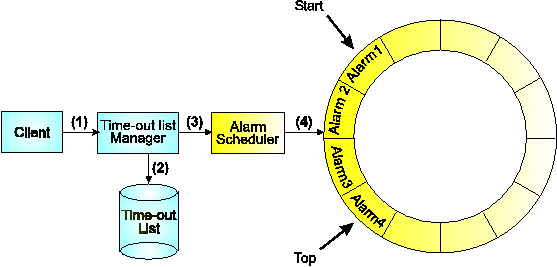
\includegraphics[width=.7\textwidth]{tomarch.png}}

%\vspace*{-0.5in}
\begin{description}
\item[(1)] Client sends requests to TOLM
\item[(2)] TOLM updates its time-out list
\item[(3)] When a time-out expires, TOLM sends an alarm request to \AS
\item[(4)] The \AS{} choses an alarm server---or waits for any
\end{description}





%%%%%%%%%%%%%%%%%%%%%%%%%%%%%%
\end{frame}
\begin{frame}[fragile]{Class TOM --- API}
%%%%%%%%%%%%%%%%%%%%%%%%%%%%%%
\noindent
\begin{tabbing}
{\bf 001} \= tom\UNDSCR{}declare(\&t1, \= 000000000 \= 0000 \kill\\
{\bf 1.}\>  /* declarations */\\
        \> TOM *tom; /* tom is the time-out manager descriptor */\\
        \> timeout\UNDSCR{}t t1, t2; /* two time-out objects, t1 and t2 */\\
        \> int my\UNDSCR{}alarm(TOM*), another\UNDSCR{}alarm(TOM*); /* two alarms */
\end{tabbing}


%%%%%%%%%%%%%%%%%%%%%%%%%%%%%%
\end{frame}
\begin{frame}[fragile]{Class TOM --- API}
%%%%%%%%%%%%%%%%%%%%%%%%%%%%%%
\noindent
\begin{tabbing}
{\bf 001} \= tom\UNDSCR{}declare(\&t1, \= 000000000 \= 0000 \kill\\
{\bf 2.}\> /* definitions */\\
        \> tom $\leftarrow$ tom\UNDSCR{}init(my\UNDSCR{}alarm);\\
        \> tom\UNDSCR{}declare(\&t1, TOM\UNDSCR{}NON\UNDSCR{}CYCLIC, TOM\UNDSCR{}SET\UNDSCR{}ENABLE, \\
        \>                 \> TIMEOUT1, DEADLINE1);  \\
        \> tom\UNDSCR{}declare(\&t2, TOM\UNDSCR{}CYCLIC, TOM\UNDSCR{}SET\UNDSCR{}DISABLE, \\
        \>                 \> TIMEOUT2, DEADLINE2);  \\
        \> tom\UNDSCR{}set\UNDSCR{}action(\&t2, another\UNDSCR{}alarm);
\end{tabbing}



%%%%%%%%%%%%%%%%%%%%%%%%%%%%%%
\end{frame}
\begin{frame}[fragile]{Class TOM --- API}
%%%%%%%%%%%%%%%%%%%%%%%%%%%%%%
\noindent
\begin{tabbing}
{\bf 001} \= tom\UNDSCR{}declare(\&t1, \= 000000000 \= 0000 \kill\\
{\bf 3.}\> /* insertion */\\
        \> tom\UNDSCR{}insert(tom, \&t1), \\
        \> tom\UNDSCR{}insert(tom, \&t2); \\
{\bf 4.}\> /* control */\\
        \> tom\UNDSCR{}enable(tom, \&t2); \\
        \> tom\UNDSCR{}set\UNDSCR{}deadline(\&t2, NEW\UNDSCR{}DEADLINE2); \\
        \> tom\UNDSCR{}renew(tom, \&t2); \\
        \> tom\UNDSCR{}delete(tom, \&t1); \\
        %\\
{\bf 5.}\> /* deactivation */\\
        \> tom\UNDSCR{}close(tom);
\end{tabbing}




%%%%%%%%%%%%%%%%%%%%%%%%%%%%%%
\end{frame}
\begin{frame}[fragile]{Class TOM --- Server-side management}
%%%%%%%%%%%%%%%%%%%%%%%%%%%%%%
\noindent
The time-out list is managed so that
\begin{itemize}
\item The top entry is the closest-to-expiration
\item All the other entries' deadlines are relative
	to the expiration of the top entry
\item A server-side protocol is used to adjust
	the list when inserting / deleting an entry
	from the top / middle / end of the list
\end{itemize}




%%%%%%%%%%%%%%%%%%%%%%%%%%%%%%
\end{frame}
\begin{frame}[fragile]{Class TOM --- Server-side management}
%%%%%%%%%%%%%%%%%%%%%%%%%%%%%%
\noindent
%\centerline{\psfig{figure=tom1.eps,width=19.0cm}}
\centerline{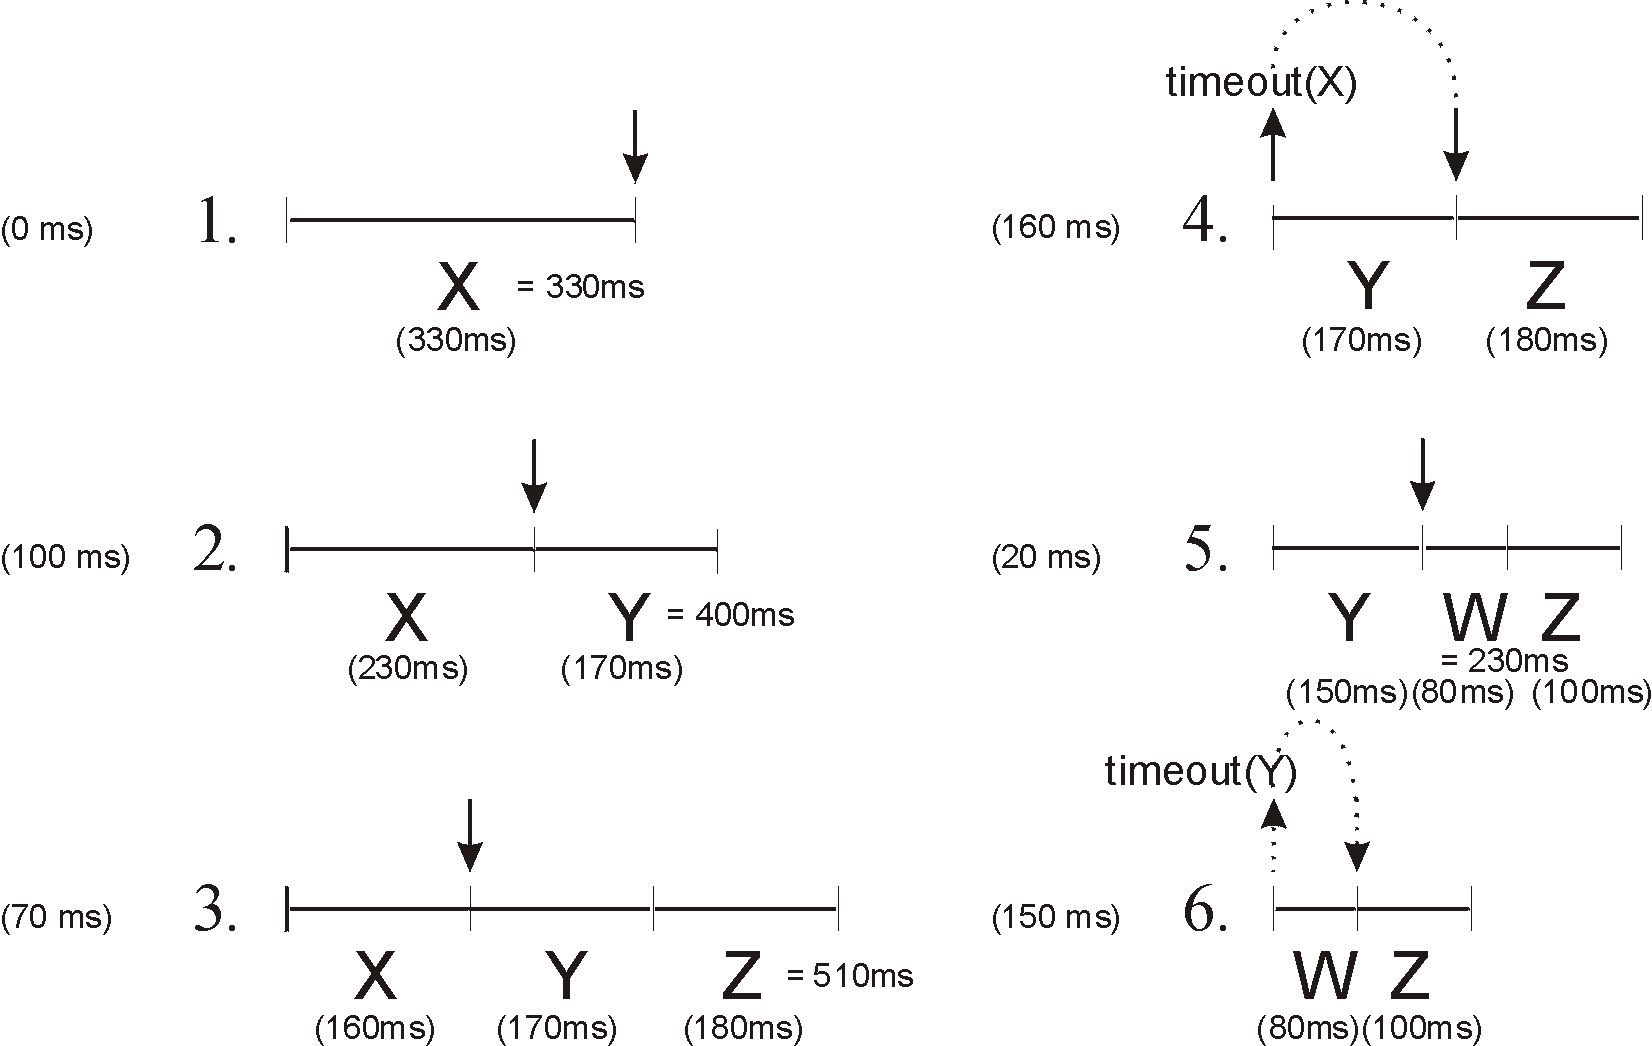
\includegraphics[width=.9\textwidth]{tom1.png}}




%%%%%%%%%%%%%%%%%%%%%%%%%%%%%
\end{frame}
\begin{frame}[fragile]{Class TOM --- Congestion}
%%%%%%%%%%%%%%%%%%%%%%%%%%%%%
\noindent
Problems:

\vspace{20pt}

\begin{itemize}
\item Time-out management implies a delay
\item Time-out detection delay is not always negligible
\item Effect of concurrent execution on the same node
\item \emph{Alarm execution delay is not negligible}
\end{itemize}




%%%%%%%%%%%%%%%%%%%%%%%%%%%%%
\end{frame}
\begin{frame}[fragile]{Class TOM --- Congestion}
%%%%%%%%%%%%%%%%%%%%%%%%%%%%%
\noindent
Alarm $\equiv$ a big source of non determinism:

\vspace{20pt}

\begin{itemize}
  \item It is defined by the user $\Rightarrow$ unknown duration
  \item Alarm often triggers some communication $\Rightarrow$ communication and
	synchronisation delays
  \item Alarms compete with each other, e.g., for a memory port or a channel
\end{itemize}
\end{frame}
%%%%%%%%%%%%%%%%%%%%%%%%%%%%%
\begin{frame}[fragile]{Class TOM --- Congestion}
%%%%%%%%%%%%%%%%%%%%%%%%%%%%%
\begin{description}
\item[$\Rightarrow$ Risk]: non negligible delay between
\end{description}


\vspace{20pt}

\[
     t_{\hbox{\small expiration}} \qquad \hbox{ and } \qquad t_{\hbox{\small alarm execution}}
\]


\vspace{20pt}

\begin{description}
\item[$\Rightarrow$ Need]: a way is needed

     \begin{itemize}
     \item to manifest, \ 
     
     \hspace*{50pt} and, if possible,
     \item to keep under control
     \end{itemize} 
     the \textbf{congestion} that is due to concurrent alarm execution.
\end{description}




%%%%%%%%%%%%%%%%%%%%%%%%%%%%%
\end{frame}
\begin{frame}[fragile]{Class TOM --- Congestion}
%%%%%%%%%%%%%%%%%%%%%%%%%%%%%
\noindent
TOM supports multiple alarm execution threads.

\vspace{20pt}

\begin{itemize}
  \item Does this solve the problem of congestion?  
  \item (Are there cases in which the problem is solved, or 
  at least, softened?)
\end{itemize}

%\noindent
%TOM works at discrete time steps: every 
%{\sf TOM\UNDSCR{}CYCLE} clock ticks, it checks whether
%something has changed and requires adjustment


%%%%%%%%%%%%%%%%%%%%%%%%%%%%%
\end{frame}
\begin{frame}[fragile]{Class TOM --- Congestion}
%%%%%%%%%%%%%%%%%%%%%%%%%%%%%
\noindent
Experiments have been performed.

\noindent
Variables: 
\begin{itemize}
\item alarm latency ($\delta$),
\item time-out deadline,
\item number of alarm threads ($\tau$),
\item \emph{competition}.
\end{itemize}


\vspace{20pt}

\noindent
{\sf TOM\_CYCLE} = 50000 clock ticks (50ms).


\vspace{20pt}

\noindent
Output: actual time of alarm minus expected time of alarm.


%%%%%%%%%%%%%%%%%%%%%%%%%%%%%
\end{frame}
\begin{frame}[fragile]{Class TOM --- Congestion}
%%%%%%%%%%%%%%%%%%%%%%%%%%%%%
\noindent
Experiment 1:
\begin{itemize}
\item $\delta\approx50\mu\hbox{s}$
\item Deadline: uniform in $[0,T]$
\item Single alarm thread
\item No competition (alarms execute \textsf{sleep()} )
\end{itemize}


\vspace{20pt}

\noindent
Deadline=50$\mu\hbox{s}$ = overhead for calling a function and copying a
20-byte message on
a DEC Alpha board running the TEX o.s.



%%%%%%%%%%%%%%%%%%%%%%%%%%%%%
\end{frame}
\begin{frame}[fragile]{Class TOM --- Congestion}
%%%%%%%%%%%%%%%%%%%%%%%%%%%%%
\noindent
%\centerline{\psfig{figure=./delays-t100-a0.ps,angle=-90,width=15.0cm}}
\centerline{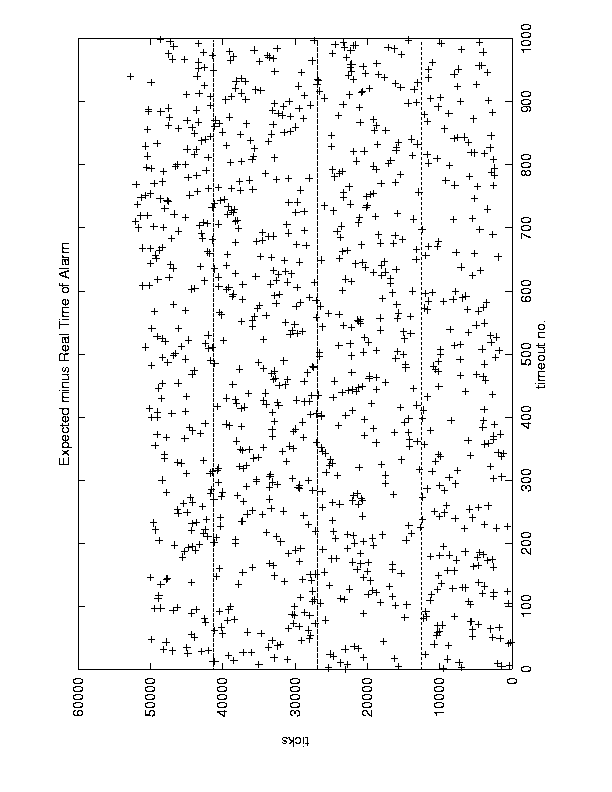
\includegraphics[width=.7\textwidth,angle=-90]{delays-t100-a0.png}}

%%%%%%%%%%%%%%%%%%%%%%%%%%%%%
\end{frame}
\begin{frame}[fragile]{Class TOM --- Congestion}
%%%%%%%%%%%%%%%%%%%%%%%%%%%%%
\begin{itemize}
\item Max=52787, min=157, avg=26892.74, stdev=14376.89
\item 20 $>$ {\sf TOM\UNDSCR{}CYCLE}
\end{itemize}

%\vfill
%\eject
%\leftheader{ }
%\rightheader{ }

%%%%%%%%%%%%%%%%%%%%%%%%%%%%%
\end{frame}
\begin{frame}[fragile]{ }
%%%%%%%%%%%%%%%%%%%%%%%%%%%%%
\noindent
%\hspace*{-0.6in}\vspace*{-1.3in}%
%\vbox{\hbox{\psfig{figure=./delays-t100-a5000.ps,angle=-90,width=13.0cm}%
%\psfig{figure=./delays-t100-a10000.ps,angle=-90,width=13.0cm}}
%\vskip-0.4in\hspace*{2.0in}\vspace*{-2.4in}\hbox{\vspace*{-1.3in}\psfig{figure=./delays-t100-a20000.ps,angle=-90,width=13.0cm}}}
%

\centerline{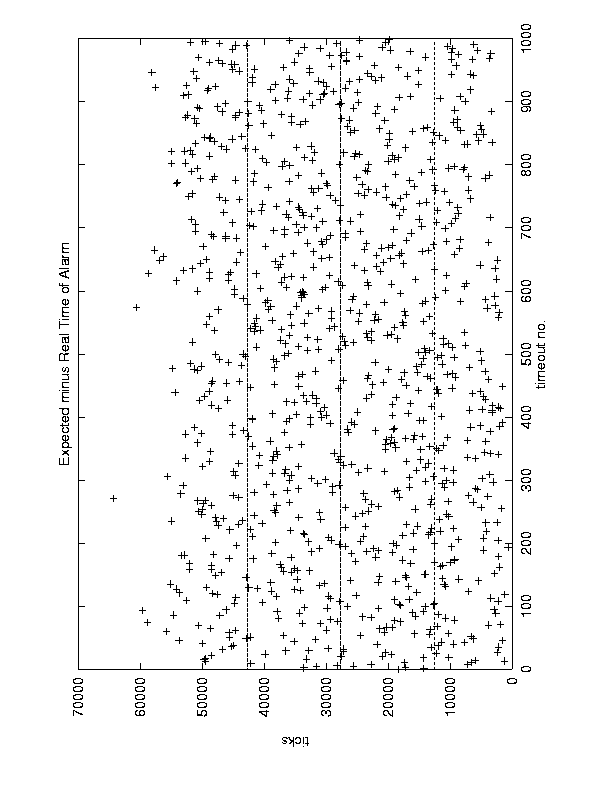
\includegraphics[width=.7\textwidth,angle=-90]{delays-t100-a5000.png}}
\end{frame}
\begin{frame}[fragile]{ }
\centerline{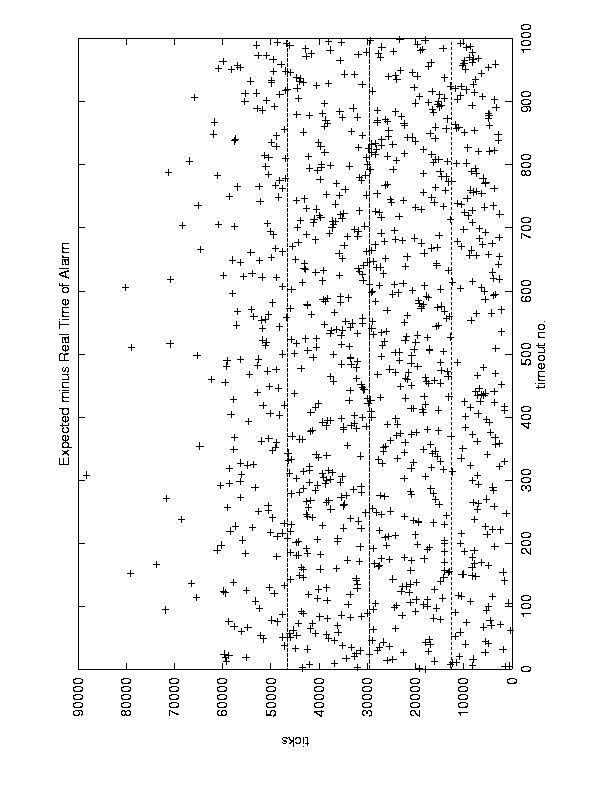
\includegraphics[width=.7\textwidth,angle=-90]{delays-t100-a10000.png}}
\end{frame}
\begin{frame}[fragile]{ }
\centerline{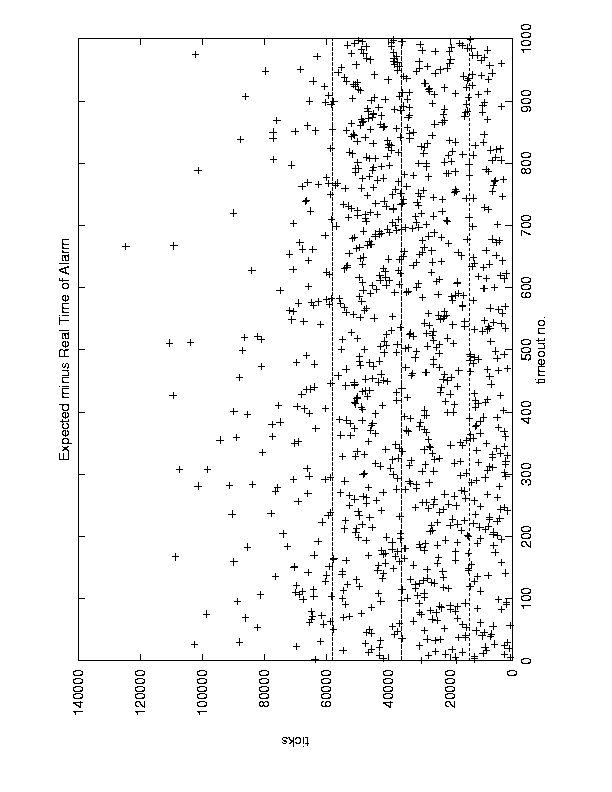
\includegraphics[width=.7\textwidth,angle=-90]{delays-t100-a20000.png}}
\end{frame}

%%%%%%%%%%%%%%%%%%%%%%%%%%%%%
\begin{frame}[fragile]{Class TOM --- Congestion}
%%%%%%%%%%%%%%%%%%%%%%%%%%%%%
\noindent
%\centerline{\psfig{figure=cmp1.ps,angle=-90,width=15.0cm}}
\centerline{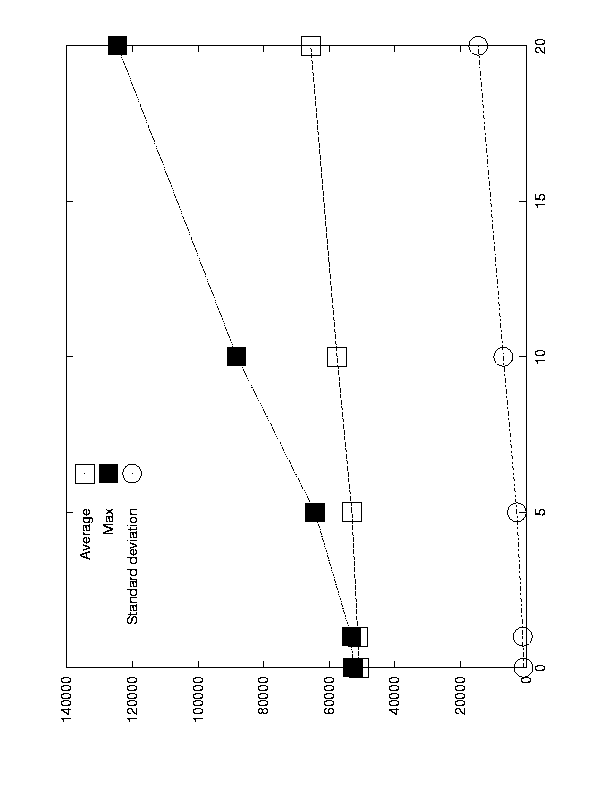
\includegraphics[width=.7\textwidth,angle=-90]{cmp1.png}}

%\vfill
%\eject
%\leftheader{ }
%\rightheader{ }

\end{frame}
%%%\begin{frame}[fragile]{ }
%%%\centerline{\includegraphics[width=.5\textwidth,angle=-90]{chaos-060.png}}
%%%\end{frame}
%%%\begin{frame}[fragile]{ }
%%%\centerline{\includegraphics[width=.5\textwidth,angle=-90]{chaos-080.png}}
%%%\end{frame}
%%%\begin{frame}[fragile]{ }
%%%\centerline{\includegraphics[width=.5\textwidth,angle=-90]{chaos-090.png}}
%%%\end{frame}
%%%\begin{frame}[fragile]{ }
%%%
%%%%%%%%%%%%%%%%%%%%%%%%%%%%%%%%
%%%\end{frame}
\begin{frame}[fragile]{ }
%%%%%%%%%%%%%%%%%%%%%%%%%%%%%
\noindent
%%\hspace*{-0.6in}\vspace*{-1.3in}%
%%\vbox{\hbox{\psfig{figure=./chaos-100.ps,angle=-90,width=13.0cm}%
%%\psfig{figure=./chaos-100-1.ps,angle=-90,width=13.0cm}}
%%\vskip-0.4in\hspace*{2.0in}\vspace*{-2.4in}\hbox{\vspace*{-1.3in}\psfig{figure=./chaos-100-2.ps,angle=-90,width=13.0cm}}}
%%
\centerline{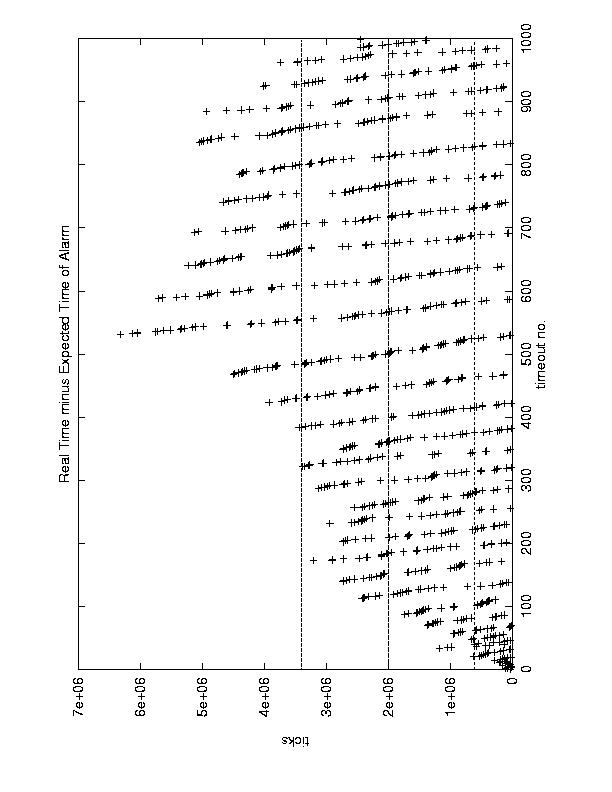
\includegraphics[width=.7\textwidth,angle=-90]{chaos-100.png}}
\end{frame}
\begin{frame}[fragile]{ }
\centerline{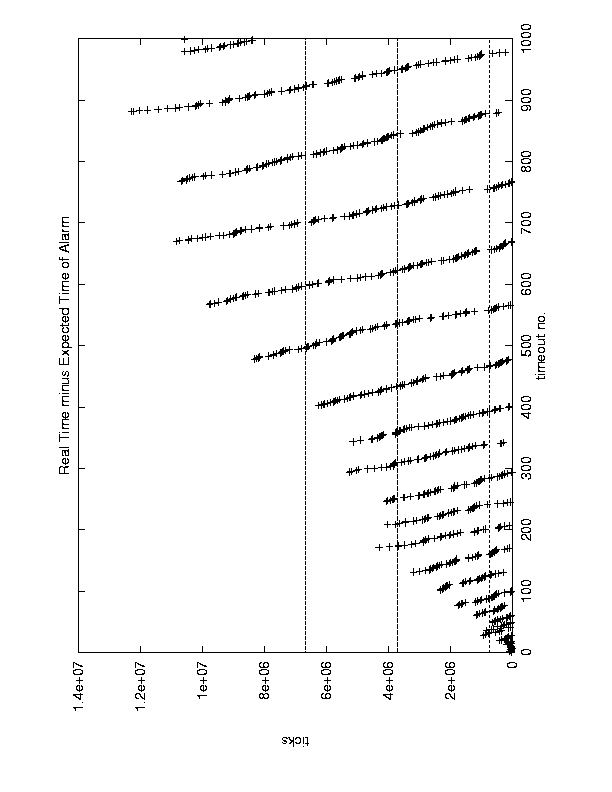
\includegraphics[width=.7\textwidth,angle=-90]{chaos-100-1.png}}
\end{frame}
%%%\begin{frame}[fragile]{ }
%%%\centerline{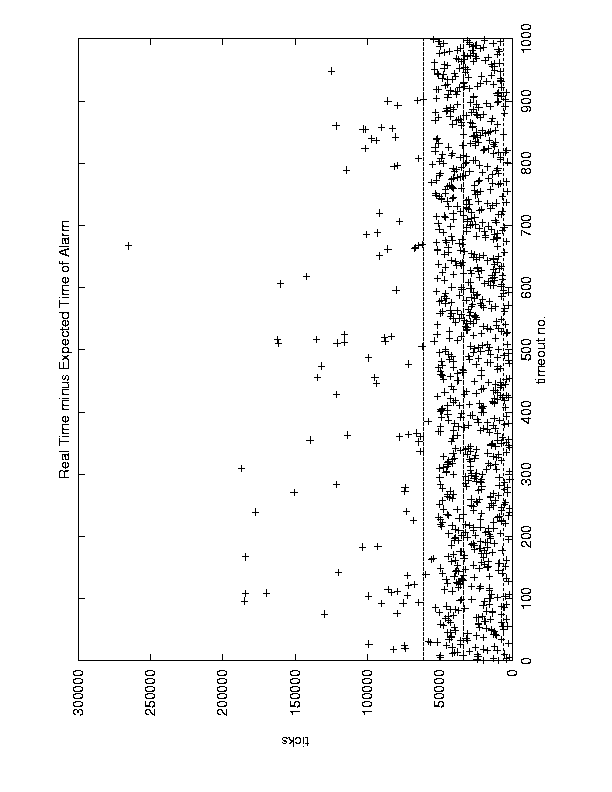
\includegraphics[width=.5\textwidth,angle=-90]{chaos-100-2.png}}
%%%\end{frame}
\begin{frame}[fragile]{ }
%%%%%%%%%%%%%%%%%%%%%%%%%%%%%
\noindent
\centerline{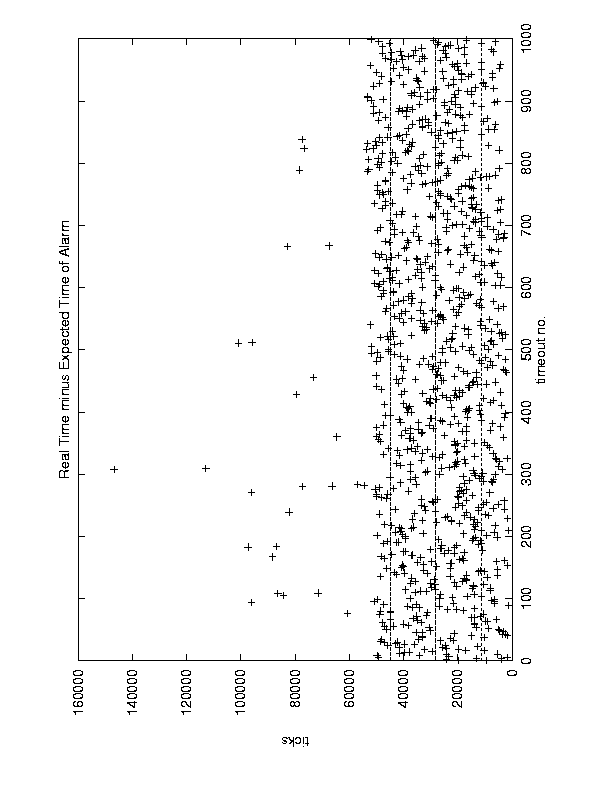
\includegraphics[width=.7\textwidth,angle=-90]{chaos-100-3.png}}
\end{frame}
\begin{frame}[fragile]{ }
\centerline{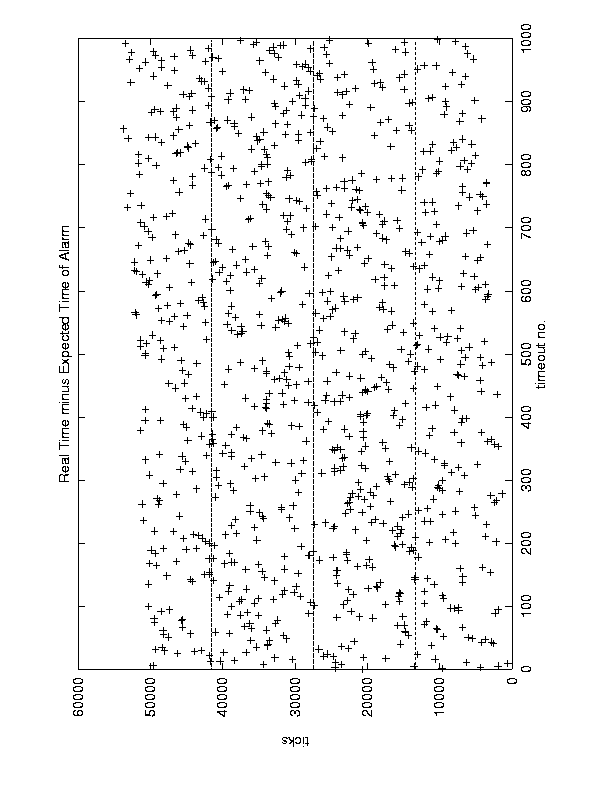
\includegraphics[width=.7\textwidth,angle=-90]{chaos-100-5.png}}
%\psfig{figure=./chaos-100-3.ps,angle=-90,width=14.0cm}
%\psfig{figure=./chaos-100-5.ps,angle=-90,width=14.0cm}


%%%%%%%%%%%%%%%%%%%%%%%%%%%%%
\end{frame}
\begin{frame}[fragile]{Class TOM --- Congestion}
%%%%%%%%%%%%%%%%%%%%%%%%%%%%%


\vspace{20pt}

\noindent
\begin{small}
\begin{tabular}{c|l|l|l|l|l|l}
$\tau$&$\mu$&$\sigma$&$exce-$&max&$\mu'$&$\sigma'$\\
&&&$ptions$&&&\\\hline
1&3692158.86&2966039.23&974&12277216&3790057.80&2943375.88\\
2&33674.46&27688.17&140&264882&83244.94&38052.06\\
3&28177.01&16801.97&54&146684&66737.87&20705.76\\
4&27621.63&14276.78&45&100260&52871.73&7358.90\\
5&27435.40&14087.22&44&53712&51375.93&1001.36\\
6&27475.84&14107.32&44&53992&51443.95&1008.77\\ \hline
\end{tabular}
\end{small}

\begin{itemize}
\item $\mu$ and $\sigma$ = average and stdev of the 1000 outcomes.
\item $\mu'$ and $\sigma'$ = average and stdev of the exceptions
\end{itemize}


%%%%%%%%%%%%%%%%%%%%%%%%%%%%%
\end{frame}
\begin{frame}[fragile]{Class TOM --- Congestion}
%%%%%%%%%%%%%%%%%%%%%%%%%%%%%
\noindent
Congestion as a result of competition! (Alarms compete for the CPU). $\delta=20$ms.


\vspace{20pt}

\begin{tabular}{c|l|l|l|l|l|l}
$\tau$&$\mu$&$\sigma$&$\gamma$&max&$\mu'$&$\sigma'$\\ \hline
1&35251.93&21667.08&226&126931&66223.70&13713.40\\
2&35533.45&21584.35&248&127403&64377.88&13803.45\\ 
3&35735.19&21606.70&250&125910&64681.21&13305.83\\ \hline
\end{tabular}


\vspace{20pt}

Conclusion: in the worst case adding alarm executors \emph{does not\/}
influence congestion!


%%%%%%%%%%%%%%%%%%%%%%%%%%%%%
\end{frame}
\begin{frame}[fragile]{Class TOM --- Congestion}
%%%%%%%%%%%%%%%%%%%%%%%%%%%%%
\noindent
Solutions: resource-specific. 
\begin{itemize}
\item Multicore CPU 
      that dynamically
      and transparently schedules the parallel execution of alarms
      on the available cores.
\item I/O $\Rightarrow$
      parallel I/O systems.
\end{itemize}


%%%%%%%%%%%%%%%%%%%%%%%%%%%%%
\end{frame}
\begin{frame}[fragile]{Class TOM --- Case Study: the Backbone}
%%%%%%%%%%%%%%%%%%%%%%%%%%%%%
\noindent
The backbone: a distributed middleware for fault-tolerant embedded
applications.


\vspace{20pt}

\noindent 
The backbone tolerates crash failures of nodes and backbone components.


\vspace{20pt}

\noindent
Based on TOM:
\begin{itemize}
\item IA\_SET\_TIMEOUT, IA\_CLEAR\_TIMEOUT
\item MIA\_SEND\_TIMEOUT, TAIA\_RECV\_TIMEOUT
\item MIA\_RECV\_TIMEOUT, TAIA\_SEND\_TIMEOUT
\end{itemize}


%%%%%%%%%%%%%%%%%%%%%%%%%%%%%
\end{frame}
\begin{frame}[fragile]{Class TOM --- Conclusion}
%%%%%%%%%%%%%%%%%%%%%%%%%%%%%
\noindent
\begin{itemize}
\item Application-level time-out support
\item Available on Windows, Parsytec EPX, TEX microkernel
\item Multi-threaded architectures $\Rightarrow$ better exploitment
      of a system's resources
\item Problem of congestion due to the concurrent execution of alarms
\item Successfully used in European projects
\item ``Algorithm of mutual suspicion''
\end{itemize}


%%%%%%%%%%%%%%%%%%%%%%%%%%%%%%%%%%%%%%%%%%%%%%%
\end{frame}
\begin{frame}[fragile]{Class FN}
\begin{itemize}
\item FN : a class for application-level input and interpretation of user-defined
      functions
\item The user types in a mathematical function. This function can be then be evaluated.
\item See \verb"https://github.com/Eidonko/FN"
\item Same principle and shape of class FILE:
\end{itemize}

\vspace{20pt}

\begin{verbatim}
FN *f;     double *x, *y, z; float d;
printf("Please, type in a function of variables x and y\n");
f = fnopen();
\end{verbatim}


%%%%%%%%%%%%%%%%%%%%%%%%%%%%%%%%%%%%%%%%%%%%%%%
\end{frame}
\begin{frame}[fragile]{Class FN}
\begin{verbatim}
/* x and y point resp. to variables FN.x and FN.y */
x = fnmemory(f, 'x');
y = fnmemory(f, 'y');

printf("Please, type in a value for x and a value for y\n");
scanf("%f", &d); *x = d;
scanf("%f", &d); *y = d;

printf("The value of your function in %lf and %lf is %lf\n",
       *x, *y, fnread());
\end{verbatim}



%%%%%%%%%%%%%%%%%%%%%%%%%%%%%%%%%%%%%%%%%%%%%%%
\end{frame}
\begin{frame}[fragile]{Class FN}
\begin{itemize}
\item Written with LEX and YACC
\item Test program on the web: Julia sets
\item Example: julia -1 1 -1 1 200, re(x,y)=x*x-y*y, im(x,y)=2*x*y+0.99) 
\end{itemize}
\end{frame}
%%%%%%%%%%%%%%%%%%%%%%%%%%%%%%%%%%%%%%%%%%%%%%%

%%{{{  Lex and YACC

%%%%%%%%%%%%%%%%%%%%%%%%%%%%%%%%%%%%%%%%%%%%%%%
\begin{frame}{Lexical and Syntactical Analysis with Lex and YACC}
The capability 
\begin{itemize}
\item to compose valid sentences in a given language, as well as
\item to verify that a given string represents a valid sentence
in a given language
\end{itemize}
builds upon two lower level capabilities:
%%%%%%%%%%%%%%%%%%%%%%%%%%%%%%%%%%%%%%%%%%%%%%%
\end{frame}

\begin{frame}[fragile]{Lexical and Syntactical Analysis with Lex and YACC}
\begin{enumerate}
\item classification: the capability of decomposing a stream
of characters into a stream of lexical entities (words,
punctuation, delimiters) (lexical analysis), and
\item verification: the capability to recognize the
syntactical correctness of a sentence, starting from a
stream of lexical entities (syntactical analysis).
\end{enumerate}


%%%%%%%%%%%%%%%%%%%%%%%%%%%%%%
\end{frame}
\begin{frame}[fragile]{Lexical and Syntactical Analysis}
%%%%%%%%%%%%%%%%%%%%%%%%%%%%%%
Given, for instance, the mathematical expression:
$$ sin (a+\sqrt(0.4)) $$


\vspace{20pt}

\begin{enumerate}
\item the first capability means translating the stream of characters
that corresponds to the above expression, i.e.,

\vspace{20pt}


({\tt 's'}, {\tt 'i'}, {\tt 'n'}, {\tt ' '},{\tt '('}, {\tt 'a'}, ...)


\vspace{20pt}

into a stream of tokens, or syntactical atoms:


\vspace{20pt}

({\tt "sin"}, {\tt '('}, {\tt "a"}, {\tt '+'}, {\tt "sqrt"}, ...)

\item the second capability is the one
that allows us to verify the syntactical correctness of the sentence,
given a certain ``grammar,'' i.e., in this case, the grammar of
well-formed mathematical formulae.
\end{enumerate}



%%%%%%%%%%%%%%%%%%%%%%%%%%%%%%
\end{frame}
\begin{frame}[fragile]{Lexical and Syntactical Analysis}

The above mentioned capabilities are experienced by the human being
as inherent and natural abilities, of which one has not even full
awareness.


\vspace{20pt}

When one has to set up, e.g., an interpreter of a computer language,
or any other software module that needs to recognize a given
structure in its input stream, then it is useful to set up
a hierarchical structure at the base of which there are tools
for lexical and syntactical analysis.


\vspace{20pt}

These tools are software systems that ease the development of
lexical and syntactical analyzers. In UNIX, for instance,
two standard utilities are available: Lex and YACC
(or their GNU equivalents: flex and bison!)

%%%%%%%%%%%%%%%%%%%%%%%%%%%%%%
\end{frame}
\begin{frame}[fragile]{Lexical and Syntactical Analysis}

Lex and YACC allow to speed up considerably the development
of parsers, translators, compilers, interpreter, conversion tools.


\vspace{20pt}

They have been especially designed for combined use and for
hosting user-defined C routines where needed.

%%%%%%%%%%%%%%%%%%%%%%%%%%%%%%
\end{frame}
\begin{frame}[fragile]{LEX: a lexical analyzer generator}

LEX may be defined as a ``tokenizator'': given a stream of
chars, LEX performs a classification of groups of contiguous
characters. These groups are called tokens, i.e., words and
symbols that are \emph{atomic\/} from the viewpoint of
syntactical analysis.


\vspace{20pt}

For instance, LEX can translate string
$ sin (a+sqrt(0.4)) $
in a set of couples ``(token, token \#)'', e.g., as follows:
\begin{itemize}
\item ``sin'', {\tt FUNCTION}
\item ``('', {\tt '('}        
\item and so forth.
\end{itemize}


\vspace{20pt}

The token \# identifies the class the token belongs to.

\end{frame}
\begin{frame}[fragile]{LEX}
LEX can be used
\begin{itemize}
\item either as a stand-alone tool, so to perform simple
translations or compute statistics on the lexycal atoms,
\item or in conjunction with a parser generator (e.g., YACC).
\end{itemize}


\vspace{20pt}

$$ \mbox{input}
 \stackrel{\mbox{\tiny LEX}}{\Rightarrow}
 \mbox{tokens / errors}
 \stackrel{\mbox{\tiny YACC}}{\Rightarrow}
                \mbox{valid / invalid sentences}
 \stackrel{\mbox{\tiny User code}}{\Rightarrow}
 \mbox{user-defined actions}
$$


%%%%%%%%%%%%%%%%%%%%%%%%%%%%%%
\end{frame}
\begin{frame}[fragile]{LEX}
LEX writes a deterministic FSA from a list of \textbf{regular expressions}
(regex). Regardless the number of rules supplied by the user, and regardless
their complexity, the LEX FSA breaks the input stream into tokens
in a time that is proportional to the length of the input stream.


\vspace{20pt}

The number of rules and their complexity only influence
\emph{the size\/} of the output source code.

%%%%%%%%%%%%%%%%%%%%%%%%%%%%%%
\end{frame}
\begin{frame}[fragile]{Structure of a LEX program}
The general structure of a LEX program is as follows:


\vspace{20pt}

\begin{quote}
[ {\em Definitions\/} ]

\pcpc

[ {\em Rules\/} ]

[ \pcpc

{\em User functions\/} ]
\end{quote}


\vspace{20pt}

{\em Definitions\/} and {\em User functions\/} can be missing.

\vspace{20pt}


Hence, the minimum size LEX program is the following one:


\vspace{20pt}

\begin{center}\pcpc\end{center}





%%%%%%%%%%%%%%%%%%%%%%%%%%%%%%
\end{frame}
\begin{frame}[fragile]{LEX}

LEX performs its classification via a list of 
{\bf regular expressions} ({\em regex\/}) that the user needs
to supply via a standard language.


\vspace{20pt}

Regex's describe \emph{patterns of characters\/} to be
located in the text. LEX reads these regex's and produces a
FSM that recognizes those patterns.

\vspace{20pt}


FSM's are indeed the simplest conceptual tool
with which to recognize words expressed by regex's.

%%%%%%%%%%%%%%%%%%%%%%%%%%%
\end{frame}
\begin{frame}[fragile]{Metacharacters in LEX}
%%%%%%%%%%%%%%%%%%%%%%%%%%%
LEX uses the same regex recognizer used by most of those UNIX tools
that do pattern matching: 
{\tt vi}, {\tt sed}, {\tt awk}, {\tt find}, {\tt grep}, 
for instance, adopt the same set of agreement based on the same set of
``metacharacters'':


\vspace{20pt}

\verb! " \ [ ] ^ - ? . * + | { } $ / ( ) % < >!


\vspace{20pt}

(Python, Perl, Java, and others, adopt slightly different sets.)



\end{frame}
\begin{frame}[fragile]{Metacharacters in LEX}

\begin{description}
\item{\tt "}
        the quotation mark operator is the simplest metacharacter:
	all the characters of a string betweeb quotation marks are
	interpreted as plain (non-meta) characters.
\item{\tt [ \ldots ]}
        Squared parentheses (pair []) specify classes of characters.
	For instance,
        {\tt [xyz]} means:
        ``{\em a single {\tt x}, {\tt y} or {\tt z} char}''

	The hyphen sign between any two chars $a$ and $b$ means that all the
	chars between ord($a$) and ord($b$) are specified.
	For instance,
        {\tt [A-Z]} means
        ``{\em any uppercase letter\/}'', while
        {\tt [A-Za-z]} means: ``{\em any letter\/}''.

	Furthermore, \verb"[\40-\176]" for instance selects
	a range of characters, that is, the one between
	$octal(40)$ and $octal(176)$.
\end{description}

%%%%%%%%%%%%%%%%%%%%%%%%%%%%%%%%%%%
\end{frame}
\begin{frame}[fragile]{Metacharacters in LEX}
%%%%%%%%%%%%%%%%%%%%%%%%%%%%%%%%%%%
\begin{description}
\item{\tt [\verb"^" \ldots ]} 
Character ``{\tt \verb"^"}'' , within the squared parentheses, means
``complementary set''.
For instance, {\tt [\verb"^"0-9]} means
        ``{\em any char but the digits\/}''.

\item{\tt \verb"\"}
	(Backslash) is the same as in the C language function
	printf.

\item{\tt .}
        (Dot) means ``{\em any character but
        {\tt '\verb"\n"'}}''.
\end{description}


%%%%%%%%%%%%%%%%%%%%%%%%%%%%%%%%%%%
\end{frame}
\begin{frame}[fragile]{Metacharacters in LEX}
%%%%%%%%%%%%%%%%%%%%%%%%%%%%%%%%%%%

\begin{description}
\item{\tt ?} The question mark goes after optional strings of
characters.
For instance, {\tt ab?c} means:
``{\em either {\tt 'ac'} or {\tt 'abc'}}''.

\item{\tt *} Postfix operator ``star'' means \emph{ZERO\/} or more
instances of a given class.
As an example, {\tt [\verb"^"a-zA-Z]*} means ``{\em zero or more
instances of non-alphabetic chars\/}''.

\item{\tt +} Postfix operator ``plus'' means \emph{ONE\/} or more
instances of a given class.
For instance,
{\tt [xyz]+} means ``{\em any non-empty string, of any size, 
consisting of any of the characters
{\tt 'x'}, {\tt 'y'} and {\tt 'z'}}'', such as e.g.
{\tt xyyyyyyzz}.
\end{description}


%%%%%%%%%%%%%%%%%%%%%%%%%%%%%%%%%%%
\end{frame}
\begin{frame}[fragile]{Metacharacters in LEX}
%%%%%%%%%%%%%%%%%%%%%%%%%%%%%%%%%%%

\begin{description}
\item{Operators {\tt ()} and {\tt \verb"|"}}. Parentheses group
a set of characters into one object. For instance,
in {\tt (xyz)+}, operator {\tt +} is applied to
string {\tt xyz}. Within a group, the OR between entities
is specified via metacharacter {\tt \verb"|"}.
For instance, 


\vspace{20pt}

\begin{center}{\tt (ab\verb"|"cd+)?(ef)*}
\end{center}


\vspace{20pt}

\noindent
means ``{\em zero or more instances of string {\tt "ef"}, possibly
preceded either by string {\tt ab} or by {\tt cd+} ({\tt c} followed
by one or more instances of {\tt d}})''.
\end{description}



%%%%%%%%%%%%%%%%%%%%%%%%%%%%%%%%%%%
\end{frame}
\begin{frame}[fragile]{Metacharacters in LEX}
%%%%%%%%%%%%%%%%%%%%%%%%%%%%%%%%%%%

\begin{description}
\item{\tt \verb"^":} This char, if not within square parentheses, means
``at begin-of-file or right after a newline.''

\item{\tt \verb"$":} This means ``at the end of a line''
or ``at end-of-file'', i.e., if the following char is either
\verb"'\n'" or {\tt EOF}.
For instance, \verb"(riga|row)$" means ``string {\tt riga}
or string {\tt row} followed either by \verb"\n" or by {\tt EOF}.

\item{\tt /}: Infix operator slash checks whether an entity is
followed by another one. For instance,
{\tt a/b} means
``character {\tt a}, only when followed by character {\tt b}''.
Note that {\tt ab/\verb"\n"} is equivalent to {\tt ab\verb"$"}.
\end{description}



%%%%%%%%%%%%%%%%%%%%%%%%%%%%%%%%%%%
\end{frame}
\begin{frame}[fragile]{Metacharacters in LEX}
%%%%%%%%%%%%%%%%%%%%%%%%%%%%%%%%%%%

\begin{description}
\item{\tt \{\}:} Curly brackets have two meanings:
        \begin{itemize}
        \item When grouping two comma-separated numbers, as in
        {\tt (xyz)\{1,5\}}, they represent a {\em multiple instance}.
	The above example means 
        ``{\em from one to five instances of
        string {\tt xyz}}''.
        \item When grouping letters, they represent the value of a
	regex alias (see further on).
        \end{itemize}

\item{\tt \%} Character {\tt \%} is {\em not\/} a metacharacter but has a special
meaning.
\end{description}


\end{frame}
\begin{frame}[fragile]{LEX Definitions}
%%%%%%%%%%%%%%%%%%%%%%%%%%%%%%%%%%%%%%%%
A LEX source file may include up to three sections; the first
one is the one including the LEX definitions. Definitions include
a list of regex's:
\begin{verbatim}
letter         [a-zA-Z]
letters        {letter}+
\end{verbatim}


\vspace{20pt}

These are the rules:
\begin{enumerate}
\item At column 1, an identifier is supplied,
\item then some blank or tab chars,
\item and finally a regex.
\end{enumerate}


\vspace{20pt}

The identifier becomes an alias for its regex.
To dereference an alias one has to put curly brackets around it.
%%%%%%%%%%%%%%%%%%%%%%%%%%%%%%%%%%%%%%%%%%%%%%%%%%%



\end{frame}
\begin{frame}[fragile]{LEX Rules}
The Rules section is mainly a list of
{\em associations\/} in the form
        \[ r\Rightarrow a \]
where $r$ is a regex and $a$ is a list of {\em actions},
i.e., user defined C language statements that are executed
when the corresponding regex is recognized.


\vspace{20pt}

For instance:

\vspace{20pt}


\begin{verbatim}
        %%
        begin        printf("{");
        end          {
                         putchar('}');
                     }
\end{verbatim}




\end{frame}
\begin{frame}[fragile]{LEX Rules : Actions}

Note: when no rule is verified, a default rule is executed:
{\tt ECHO}.


\vspace{10pt}

\noindent
(The FSA written by LEX has a  {\tt switch} statement with a {\tt default: ECHO;}.)


\vspace{10pt}

\begin{itemize}
\item This means that, e.g., there is no need to supply rules for
the so called ``literal tokens,'' i.e., single characaters whose
token number is equal to their ASCII code.

\item
To ``sift out'' some portion of the input, one needs to recognize it
and to associate a null action to it.
\end{itemize}


\vspace{10pt}

To remove newline characters:
\begin{verbatim}
        %%
        \n        ;
\end{verbatim}
\end{frame}

\begin{frame}[fragile]{LEX Rules : Actions}

Some ``simple transformations'' can be useful in order
to facilitate the import of a file.


\vspace{20pt}

Some word processors, such as Word, regard paragraphs as a single line and
separate paragraphs with \verb"\n".


\vspace{20pt}

The following LEX script converts every single  \verb"\n" into character space.

\begin{verbatim}
    %%
    \n\n        ECHO;
    \n          putchar(' ');
\end{verbatim}


\end{frame}
\begin{frame}[fragile]{LEX Rules : Variables}
When a regex is recognized, the corresponding string (the token)
is copied in a 
{\tt char*} called {\tt yytext}.
This is true also for literal tokens.


\vspace{20pt}

This script is similar to the previous one:
\begin{verbatim}
    %%
    [^\n]\n[^\n]  { putchar(yytext[0]);
                    putchar(' ');
                    putchar(yytext[2]);
                  }
\end{verbatim}


\vspace{20pt}

Action {\tt ECHO} is actually a {\tt \#define}:
\begin{verbatim}
        #define ECHO puts(yytext)
\end{verbatim}
%%%%%%%%%%%%%%%%%%%%%%%%%%%%%%



\end{frame}
\begin{frame}[fragile]{LEX Rules : Variables}
Variable
{\tt int yyleng} is the number of characters of the string
which verifies the current rule; in other words,
\begin{center}\tt yyleng == strlen(yytext)\end{center}


\vspace{20pt}

For instance:\label{digalpoth}
\begin{verbatim}
%%
[0-9]+           dig += yyleng;
[a-zA-Z]+        alp += yyleng;
(.|\n)           oth++;
\end{verbatim}
%%%%%%%%%%%%%%%%%%%%%%%%%%%%%%

\end{frame}
\begin{frame}[fragile]{LEX Rules : Variables}
The above program has some bugs:


\vspace{20pt}

\begin{enumerate}
\item Variable {\tt dig} etc.
have not been declared.
\item No output message is provided at the end.
\end{enumerate}


\vspace{20pt}

LEX produces a C program. No checks are done on the
correctness of this program. It may also contain syntax errors
in the actions (actions are simply copied as strings into
the output program.)
%%%%%%%%%%%%%%%%%%%%%%%%%%%%%%



%%%%%%%%%%%%%%%%%%%%%%%%%%%%%%
\end{frame}
\begin{frame}[fragile]{LEX Rules : Functions}
A number of functions are available to the LEX user:


\vspace{20pt}

\begin{center}\tt yymore()\end{center}
Next string is attached to the current value of
{\tt yytext}.


\vspace{20pt}

\begin{verbatim}
%%
\"[^"]*   {
           if (yytext[yyleng-1] == '\\')
               yymore();
           else
               do_that(yytext);
          }
\end{verbatim}

%%%%%%%%%%%%%%%%%%%%%%%%%%%%%%
\end{frame}
\begin{frame}[fragile]{LEX Rules : Functions}
\begin{verbatim}
%%
\"[^"]*   {
           if (yytext[yyleng-1] == '\\')
               yymore();
           else
               do_that(yytext);
          }
\end{verbatim}

\verb'        '\verb*'"he said \"hi\"."'

\verb'        '\verb*'"he said \'

\verb'        '\verb'          "hi\'

\verb'        '\verb'              "."'

%%%%%%%%%%%%%%%%%%%%%%%%%%%%%%


\end{frame}
\begin{frame}[fragile]{LEX Rules : Functions}

\begin{center}\tt yyless()\end{center}
``Sends back'' a given number of characters.


\vspace{20pt}

\begin{verbatim}
%%
=-[a-zA-Z] {
           printf("Operator =- is ambiguous: ");
           printf("not recognized.\n");
           yyless(yyleng-2);
           manage_assignment();
           }
\end{verbatim}


\vspace{20pt}

(In the early days of C, {\tt a =- b} had the same meaning of
{\tt a -= b}).


\vspace{20pt}

{\tt yyless($x$)} pushes back onto the input $\hbox{\tt yyleng}-x$ characters.



\end{frame}
\begin{frame}[fragile]{LEX Rules : Functions}

\begin{description}\item{\tt int input()} reads the next input character.
(Character {\tt NULL} [that is, {\tt (int)0}] is interpreted 
as end-of-file condition)
\item{\tt void output(char c)} writes {\tt c} onto the output stream
\item{\tt void unput(char c)} ``pushes back'' {\tt c} into the input stream.
\end{description}


\vspace{20pt}

The user can choose between a standard version of these functions
or make use of his/her own functions with the same name and
prototype.



\end{frame}
\begin{frame}[fragile]{LEX Rules : Functions}
\begin{center}\tt int yywrap(void)\end{center}\label{yywrap}


\vspace{20pt}

This system (or user-) function is called when an {\tt EOF}
is encountered. The system version of this function returns
{\tt 1}, which means ``end of processing.''
The user can substitute this function with a new version
which, if it returns {\tt 0}, let the execution
continue until a new  {\tt EOF} is encountered. 


\vspace{20pt}

This way it is possible, e.g., to process more than one
input file during the same run.


\vspace{20pt}

Furthermore, {\tt yywrap()} allows the user to specify
end-of-job functions (for instance, printing of the
output and so forth.)
%%%%%%%%%%%%%%%%%%%%%%%%%%%%%%



\end{frame}

\begin{frame}[fragile]{LEX Rules}
LEX adopts two steps to select which user rule to apply:


\vspace{20pt}

\begin{enumerate}
\item The rule that recognizes the largest string is always preferred.
\item If more than one rule recognize largest strings, it is chosen
      the rule the user has specified first in the LEX script.
\end{enumerate}
\end{frame}

%\begin{frame}[fragile]{LEX Rules}
%
%An example follows:
%
%\begin{verbatim}
%    %%
%    integer         printf("1");
%    [a-z]+          printf("2");
%    (.|\n)          ;
%\end{verbatim}
%
%Dato ad esempio l'input {\tt "ABC\underline{integers}XY\underline{integer}ABC"},
%Lex produce la stringa {\tt "21"}.
%
%$\Leftarrow$: (motivazione)
%
%$\Leftarrow$: (scambio della prima rule con la seconda)
%\end{frame}


\begin{frame}[fragile]{LEX Rules}
Within a same rule, LEX returns the largest possible string:


\vspace{20pt}

\begin{verbatim}
    %%
    \'.*\'   { yytext[0] = '[';
               yytext[yyleng-2] = ']';
               printf("%s",yytext);
             }
\end{verbatim}


\vspace{20pt}

produces a program that, once read string


\vspace{20pt}

{\tt 'hi' -said- 'how are you?'}

\vspace{20pt}


writes the following string on the output:


\vspace{20pt}

{\tt [hi' -said- 'how are you?]} 


\end{frame}
\begin{frame}[fragile]{LEX Rules}

When LEX selects which rule to execute, it
creates an ordered list of possible candidates. The one
to be executed is the one on top. When the action includes macro
\begin{center}\tt REJECT;\end{center}
the following two actions take place:
\begin{enumerate}
\item the input string is sent back onto the input stream;
\item the rule is removed from the list. The rule that is selected
is therefore the new top one.
\end{enumerate}


\end{frame}
\begin{frame}[fragile]{LEX Rules}
\noindent
{\tt REJECT} is useful, e.g., to count all the
``digrams'' in a given text:


\vspace{20pt}

\begin{verbatim}
%%
[A-Z][a-z] {   digram[yytext[0]][yytext[1]]++;
               REJECT;
           }
(.|\n)     ;
\end{verbatim}


\vspace{20pt}

each digram in the text is located by the first rule, because
it returns a string of \emph{two\/} characters while the second
one returns a string of just one character.


\vspace{20pt}

{\tt REJECT} writes back the two characters of the digram onto stdin
and ``fires'' the first rule. The second one is executed.
A character is removed from the input stream.


\end{frame}
\begin{frame}[fragile]{LEX Rules}
\label{digram1}
\begin{verbatim}
%%
[a-z][a-z] {  extern int dig[26][26];
              dig[yytext[0]-'a'][yytext[1]-'a']++;
              REJECT; }
(.|\n)     ;
%%
int dig[26][26];
int yywrap() { int i, j;
        for (i=0; i<26; i++)
          for (j=0; j<26; j++)
             if (dig[i][j])
                printf("digram [%c%c] = %d\n",
                            'a'+i,'a'+j, dig[i][j]);
        return 1;
}
\end{verbatim}


\end{frame}
\begin{frame}[fragile]{Output stream in LEX}

LEX allows to include in the output C source code
any useful information (header files, declaration of
global variables and so forth.)


\vspace{20pt}

Inclusion can be done in three ``zones'' of the output
source file:
\begin{enumerate}
\item at the beginning of the file, that is, before any of the functions,
\item at the beginning of function {\tt yylex()},
\item at the end of the file.
\end{enumerate}


\end{frame}
\begin{frame}[fragile]{Output stream in LEX}
The three zones in the output source code correspond to the following
zones of the LEX script:
\begin{enumerate}
\item In {\em Definitions},
\item On top of {\em Rules\/}, i.e., right after the first \pcpc{};
\item In {\em User Functions}.
\end{enumerate}


\end{frame}
\begin{frame}[fragile]{Output stream in LEX}
Case {\bf 3} is trivial. For 
{\bf 1} and {\bf 2}, we need to distinguish the text to be processed
by LEX from the text that needs to be copied verbatim in the output file.
To do this, one can follow any of these ways:
\begin{itemize}
\item {\tt [ \verb"\"t]+.*} \ (at least a blank space or tab character
at column zero, then the data to be flushed onto the output file.)
\item Anything between \verb"%{" and \verb"%}".
\end{itemize}

\end{frame}
\begin{frame}[fragile]{Practical use of LEX}
\begin{enumerate}
\item {\tt lex {\em source}.l}
\item {\tt gcc lex.yy.c -ll}
\item {\tt a.out < input}
\end{enumerate}


\end{frame}
\begin{frame}[fragile]{Practical use of LEX}
File {\tt lex.yy.c} contains function  {\tt yylex()}
i.e., the actual scanner. Compiling
{\tt lex.yy.c} with the system library {\tt libl.a},
a {\tt main()} function is automatically supplied
which calls function {\tt yylex()}.


\vspace{20pt}

The user can substitute this default {\tt main()} with
one of their own design.


\vspace{20pt}

Doing this, one can choose between either
automatically generating an executable or
``piping'' LEX output to other programs---for instance,
syntactical analyzers.


\end{frame}
\begin{frame}[fragile]{LEX: Selection of a scanning context}
Writing a lexical analyser can be made easier when using
more than one scanning context. A scanning context is a
set of scanning rules that apply within a certain context
and do not apply in other contexts.


\vspace{20pt}

Classical example: the presence of string
\verb"/*" may imply the activation of a set of rules that
are completely different from the standard rules. The
same applies for constant strings.


\vspace{20pt}

The context switch can be done in various ways:
\begin{itemize}
\item flag method, \item start conditions,
\item multiple scanners
\end{itemize}

\end{frame}
\begin{frame}[fragile]{Practical use of LEX}
\begin{center}{Selection of a scanning context: flag method}
\end{center}


\vspace{20pt}

\begin{verbatim}
        int flag=0; /* starts with a tab! */
%%
"/*"    flag=1;
"*/"    flag=0;
.       |
\n      if (flag==0) putchar(*yytext);
\end{verbatim}


\vspace{20pt}

It is the programmer's responsibility to use the method in a coherent way.

\end{frame}
\begin{frame}[fragile]{Practical use of LEX}
\begin{center}{Selection of a scanning context: start conditions/multiple scanners}
\end{center}


\vspace{20pt}

An identifier, called ``start condition,'' is associated
to some rules. The rule becomes part of the lexical context
identified by the start condition. The current start condition
can be changed at any time:


\vspace{20pt}

\begin{verbatim}
any       (\n|.)
%start    REMARK
%%
"/*"          BEGIN REMARK;
"*/"          BEGIN 0;
<REMARK>{any} ;
{any}         putchar(*yytext);
\end{verbatim}


\vspace{20pt}

Finally, one can write multipler scanners and then activate
the one corresponding to the current context.

\end{frame}
\begin{frame}[fragile]{LEX: Definitions}
Apart from regex aliases, in {\em Definitions\/} it is possible to specify
``internal codes'' for any character:


\vspace{20pt}

\begin{verbatim}
%T
1         Aa
2         Bb
.....
26        Zz
%T
\end{verbatim}


\vspace{20pt}

This allows definitions such as
\verb"[Dd][Oo][Uu][Bb][Ll][Ee]"
to be avoided when the case of letters in the input is not important.


\vspace{20pt}

Note: code 0 is illegal;
codes greater than $2^{\hbox{\tiny\tt sizeof(char)}\times8}-1$ are illegal;
once a table has been defined, LEX only recognizes the characters in that table. 

\end{frame}
\begin{frame}[fragile]{Practical use of LEX: exercises}
\begin{itemize}
\item Write a CGI script that translates extended HTML to plain HTML
	\begin{itemize}
	\item Clause $<$IF$>$ $<$THEN$>$ $<$ELSE$>$ $<$FI$>$ $<$REXEC$>$ ...
	\item $<$IF$>$REMOTE\_ADDR = 134.58.63.88$<$THEN$>$ ... $<$ELSE$>$ ... $<$FI$>$
	\end{itemize}
\item Write a scanner to recognize the lexical atoms of a programming language
\end{itemize}

\end{frame}
\begin{frame}[fragile]{Practical use of LEX: exercises}
\begin{itemize}
\item Write a simple ``translator'' for a Pascal-like pre-processor
\begin{verbatim}
BEGIN {
END   }
EQ    ==
IF    if(
THEN  )
END;  }
END.  }
\end{verbatim}
\end{itemize}

\end{frame}
\begin{frame}[fragile]{LEX: bibliography}

\begin{enumerate}
\item \label{lex} M.E Lesk, E. Schmidt, {\em LEX - a lexical  analyzer
generator\/},  in  ConvexOs  Tutorial  Papers,  CCC,  1993.  
\item \verb"http://www.combo.org/lex_yacc_page/" : the lex \& yacc page
\end{enumerate}
%%}}}

%%{{{  YACC
\end{frame}
\begin{frame}[fragile]{Syntactical Analysis with YACC}
\begin{center}
YACC : {\em Yet Another Compiler-Compiler\/}
\end{center}
YACC has been defined by its authors as a system for describing
the input structure of a program.


\vspace{20pt}

The YACC programmer is required to supply:
\begin{enumerate}
\item the syntactical structure of the input 
\item C code to be executed when the syntax rules are recognized.
\end{enumerate}


\vspace{20pt}

On the basis of these data, YACC writes a C program with a
parsing routine.


%%%%%%%%%%%%%%%%%%%%%%%%%%%%%%
\end{frame}
\begin{frame}[fragile]{YACC}
%%%%%%%%%%%%%%%%%%%%%%%%%%%%%%
The parsing routine calls a lower level routine, called {\tt yylex()},
in order to get the next lexical atoms in the input stream.


\vspace{20pt}

YACC works with grammars of type
{\bf LALR(1)}, plus rules to solve ambiguities.


%%%%%%%%%%%%%%%%%%%%%%%%%%%%%%
\end{frame}
\begin{frame}[fragile]{YACC}

The general structure of a YACC script
strictly follows the one of a LEX script:


\vspace{20pt}

\begin{quote}
[ {\em Definitions\/} ]

\pcpc

{\em Rules \& Actions}

[ \pcpc

{\em User functions\/} ]
\end{quote}

%%%%%%%%%%%%%%%%%%%%%%%%%%%%%%
\end{frame}
\begin{frame}[fragile]{YACC}
In particular, the structure of {\em Rules \& Actions\/}
is similar to the corresponding section of a LEX script:
it includes a set of \emph{grammar rules}, plus  \emph{actions\/}
that are associated to each rule.


\vspace{20pt}

Each time a rule is recognized, the corresponding actions are executed.


\vspace{20pt}

Actions may return values and use the values returned by other actions.

%%%%%%%%%%%%%%%%%%%%%%%%%%%%%%
\end{frame}
\begin{frame}[fragile]{YACC}

YACC rules have the following structure:
\begin{center}\em lhs {\tt :} rhs {\tt ;}
\end{center}


\vspace{20pt}

where {\em lhs\/} is a non-terminal symbol and {\em rhs\/}
is a sequence of 
\underline{zero} or more terminal or non-terminal symbols,
``literals,'' and actions.


\vspace{20pt}

Identifiers for terminal and non-terminal symbols follow the
rules of the C language, with the addition that character
{\tt '.'} is considered as a letter.


\end{frame}
\begin{frame}[fragile]{YACC}
%%%%%%%%%%%%%%%%%%%%%%%%%%%%%%
A literal is a constant character defined as follows:


\vspace{20pt}

\begin{verbatim}
literal : QUOTE char QUOTE 
        | QUOTE BACKSLASH char QUOTE
        | QUOTE BACKSLASH od od od QUOTE
         ;
\end{verbatim}


\vspace{20pt}

\noindent
(being {\tt QUOTE} character \verb'"' and {\tt od} an octal digit.)


\vspace{20pt}

Character ``\verb"|"'' is an OR. It is used when more than one rule
has the same  {\em lhs}.


\end{frame}
\begin{frame}[fragile]{YACC: user definitions}
As with LEX, the parentheses
 \verb"%{" and \verb"%}" allow to include in the output of YACC
 any C source code. This code is global with respect to the
 parser function and to the user functions.


\vspace{20pt}

YACC uses a number of identifiers starting with
``{\tt yy}'' for internal purposes. This prefix must be avoided.


\end{frame}
\begin{frame}[fragile]{YACC: token declaration}
Lexical atoms (the tokens) must be explicitly declared in 
{\em Definitions}. This is done, for instance,
by writing one or more lines
such as the following one:


\vspace{20pt}

\begin{center}\em
\verb"%token" nome${}_1$  nome${}_2$  $\dots$
\end{center}


\vspace{20pt}

All the symbols that have not declared as tokens are
implicitly declared as non-terminals (NTs). 

\vspace{20pt}


Note: each NT must be the {\em lhs\/} of at least one rule.

%%%%%%%%%%%%%%%%%%%%%%%%%%%%%%

\end{frame}
\begin{frame}[fragile]{YACC: specification of the start symbol}
The declaration of the start symbol of the grammar may be done as follows:

\vspace{20pt}


\begin{center}\em
\verb"%start" name
\end{center}


\vspace{20pt}

in {\em Declarations}. If this specification is missing,
it is assumed that the start symbol is the
{\em lhs\/} of the first grammar rule specified by the user.


%%%%%%%%%%%%%%%%%%%%%%%%%%%%%%

\end{frame}
\begin{frame}[fragile]{YACC: the endmarker token}
A special token marks the end-of-input. This is called
\endmarker{} in YACC lingo.


\vspace{20pt}

If the tokens encountered between the start of processing
and the \endmarker{} (not including the latter)
{\em verify\/} the start symbol, then
the parsers successfully stops processing after having read
the \endmarker.


\vspace{20pt}

Reading the \endmarker{} before the start symbol is verified
leads to an error.

%%%%%%%%%%%%%%%%%%%%%%%%%%%%%%

\end{frame}
\begin{frame}[fragile]{YACC: actions}

Within each rule, the programmer can specify some \emph{actions\/}
to be executed each time that rule is recognized while analysing
the input stream.


\vspace{20pt}

Actions may return values and use the values returned by other actions.


\vspace{20pt}

Also the tokens returned by {\tt yylex()} may have values.


\vspace{20pt}

Actions are a number of C statements between curly brackets. Each
action can return a value by setting variable
\verb"$$". For instance:


\vspace{20pt}

\verb"   { action(); $$=1; }"

\vspace{20pt}

returns 1.



\end{frame}
\begin{frame}[fragile]{YACC: actions}
Also the rules may return values. This value is either
the value of the first component or the value of variable  \verb"$$".
For instance:


\vspace{20pt}

\verb" A : B;"


\vspace{20pt}

is equivalent to


\vspace{20pt}

\verb" A : B { $$ = $1; } ;"

%%%%%%%%%%%%%%%%%%%%%%%%%%%%%%


\end{frame}

\begin{frame}[fragile]{YACC: actions}
The following example shows how it is possible
to use the values returned by previous rules.


\vspace{20pt}

\begin{verbatim}
    expr    :   '('   expr   ')'
                {    $$ = $2;   }
            ;
\end{verbatim}


\vspace{20pt}

In other words, \$$i$  is the value returned by  RHS$[i]$.
\end{frame}

\begin{frame}[fragile]{YACC: actions}
An example follows:


\vspace{20pt}

\begin{verbatim}
expr :   expr    infix_op     expr
         {  $$ = node( $2, $1, $3);  }
     ;
\end{verbatim}


\vspace{20pt}

For instance, function {\tt node()} may allocate an object and return
its address. This is used when building syntax analysis trees.

\vspace{20pt}


Note: values returned by rules and actions are integers by default.

%%%%%%%%%%%%%%%%%%%%%%%%%%%%%%

\end{frame}
\begin{frame}[fragile]{YACC: function {\tt yylex()}}
Function {\tt yylex()} returns an integer---the token number.
This number is either a literal (when in $[0,255]$) or
a symbolic constant $s>256$ that describes the lexical ``class''
the recognized string belongs to. For instance,
{\tt NUMBER}. 


\vspace{20pt}

Function {\tt yylex()} also returns the actual string that
was found in the input. That string is kept in variable


\vspace{20pt}

\begin{center}\tt extern {\bf X} yylval;\end{center}


\vspace{20pt}

where {\bf X} is either {\tt int} or can be defined by the user.


\vspace{20pt}

\begin{verbatim}
%%
[0-9]+  { yylval=atoi(yytext); return NUMBER; }
\end{verbatim}

%%%%%%%%%%%%%%%%%%%%%%%%%%%%%%


\end{frame}
\begin{frame}[fragile]{YACC: token numbers}
The choice of which integers to use with token can be done
\begin{description}
\item{\em automatically\/} by YACC, which associates the integers
from 257 one by one to the tokens that have been declared with
the \verb"%token" keyword.
\item{\em implicitly\/} for literals, to which is associated
the ASCII code.
\item{\em explicitly\/} by the YACC programmer, who can
associate an integer greater than 0 after the name of a token or a literal
in section \emph{Declarations}.
\end{description}

%%%%%%%%%%%%%%%%%%%%%%%%%%%%%%
\end{frame}

\begin{frame}[fragile]{YACC: token numbers}
Token numbers must be different.


\vspace{20pt}

When executing {\tt yacc} with the {\tt -d} option, a header file
is created, called
{\tt y.tab.h}, which contains all the token numbers.
This file can be included, e.g., in the LEX script as follows:


\vspace{20pt}

\begin{verbatim}
%{
#include "y.tab.h"
%}
\end{verbatim}


\vspace{20pt}

Note: the C program produced by LEX can be either compiled separately
or even included in the YACC output program by specifing in
\emph{User functions\/} the following statement:
\begin{verbatim}
#include "y.tab.c"
\end{verbatim}
\end{frame}

\begin{frame}[fragile]{YACC: choice of the lexical analizer}

LEX is usually ``\emph{the\/}'' lexical analizer to be used with
YACC. Under specific circumnstances, though, LEX may be
less suited than an ad-hoc lexical analizer. For instance, when
recognizing a Fortran grammar, it may be difficult with LEX
to express conditions that depend, e.g., on the column
where a given command starts.
\end{frame}

\begin{frame}[fragile]{YACC algorithm}
YACC produces a FSM with two parallel stacks representing
states and values:

\vspace{20pt}


\begin{verbatim}
short	yyssa[YYINITDEPTH]; /* the state stack */
YYSTYPE yyvsa[YYINITDEPTH]; /* the value stack */
#define YYPOPSTACK   (yyvsp--, yyssp--)
\end{verbatim}


\vspace{20pt}

The parser can read and store the next input token
[this is called
look ahead token (\lat) in YACC lingo.]


\vspace{20pt}

The state stack,
$S$, is a vector of integers. The current state is always
TOP$(S)$.


\vspace{20pt}

Initially \lat $=\Lambda$, {\tt sp=0}, TOP$(S)$=0.
\end{frame}

\begin{frame}[fragile]{YACC algorithm}
The FSM mainly makes use of four basic actions:
\shift, \reduce, \accept{} ed \error.
(A fifth action, \goto, is actually a \shift).


\vspace{20pt}

The main loop of YACC is in two basic steps:


\vspace{20pt}

\begin{enumerate}
\item On the basis of TOP$(S)$:

      is  \lat{} required? Yes: read \lat{} (call {\tt yylex()} and so forth.)
\item On the basis of both TOP$(S)$ and \lat:

      choose next action.
\end{enumerate}
\end{frame}

\begin{frame}[fragile]{YACC algorithm}
YACC uses a symbolic language to describe the structure of the output FSM.
Running YACC with the option

$$\hbox{\tt -v}$$

a file called {\tt y.output} is produced. This file contains
a number of statements in the form:


\vspace{20pt}

\begin{center}\em
symbol  opcode  operand
\end{center}

or
\begin{center}\em
.  opcode  operand
\end{center}


\vspace{20pt}

where {\em opcode} is {\tt shift} or {\tt reduce} and so forth,
and {\em operand} is an integer that represents either a
\emph{state\/} or a
\emph{grammar rule}.
\end{frame}

\begin{frame}[fragile]{YACC algorithm}
Reading
{\tt y.output} is a way to ease up the debugging of a YACC program.
Now it is described how to interpret {\tt y.output}.


\vspace{20pt}

\begin{center}\fbox{\shift}\end{center}
\begin{center}\em  symbol    {\tt shift}  new-state \end{center}


\vspace{20pt}

Within the current state:


\vspace{20pt}

\begin{itemize}
\item if \lat $=\Lambda$, read(\lat).
\item if \lat={\em symbol}, push({\em new-state\/}, {\tt yylval}).
\item \lat{} $\leftarrow\Lambda$
\end{itemize}
\end{frame}

\begin{frame}[fragile]{YACC algorithm}

Push and pop are executed in parallel on the two stacks.


\vspace{20pt}

``{\tt .}'' means ``any symbol''.
\end{frame}

\begin{frame}[fragile]{YACC algorithm}

\shift{} makes the stacks grow. The dual action is


\vspace{20pt}

\begin{center}\fbox{\reduce}\end{center}
\begin{center}\em  {\tt .}   {\tt reduce}  rule \end{center}


\vspace{20pt}

\reduce{} comes into play the moment the parser has finished
the scan of an
{\em rhs\/} and needs to replace it with the non-terminal that is
{\em lhs\/} in the corresponding rule.


\vspace{20pt}

Usually \reduce{} is unconditioned, though it may also take the form
\begin{center}\em  symbol   {\tt reduce}  rule \end{center}


\vspace{20pt}

Rule is an integer identifying a given rule.
\end{frame}

\begin{frame}[fragile]{YACC algorithms: reduction algorithm}
\begin{itemize}
\item the action corresponding to the rule is executed;
\item {\tt for (i=0; i< $\nu$({\em rhs}); i++) pop();}
\item TOP$(S)$ (the so-called ``{\em uncovered state\/}'') is inspected
\item ...when a command like this:

\[ \hbox{\tt{\em lhs\/} goto {\em x}} \]
is found, the following command is executed:
\[ \hbox{\tt push({\em x})}. \]
\end{itemize}


\vspace{20pt}

\goto{} differs from \shift{} in that it does not
erase the \lat.
\end{frame}

\begin{frame}[fragile]{YACC algorithms: reduction algorithm}
\reduce{} purges the states corresponding to the {\em rhs\/}
and lets the YACC FSM behave as if it had encountered
symbol {\em lhs}.


\vspace{20pt}

As a special case, void rules such as
$$\verb"A : ;"$$
mean: 


\vspace{20pt}

\begin{itemize}
\item do not execute any pop();
\item inspect the current state TOP$(S)$\ldots
\item \ldots looking for an instruction such as

\verb" A goto" $x$
\end{itemize}
\end{frame}

\begin{frame}[fragile]{YACC algorithms: reduction algorithm}

When a rule is encountered, right before executing a  \reduce{},
the action associated with that rule is executed.


\vspace{20pt}

This action has access to all the values of its components
by means of variables \verb"$1", \verb"$2" and so forth.


\vspace{20pt}

These numbers represent displacements within the value stack.
\end{frame}

\begin{frame}[fragile]{YACC algorithm}
\begin{center}\fbox{\accept}\end{center}
\begin{center}\tt
     if (\lat{} == \endmarker) return OK;
\end{center}


\vspace{20pt}

i.e., if the entire input has been inspected and it verifies
the rules, then conclude with success.

\begin{center}\fbox{\error}\end{center}
If in the uncovered state there is no valid next state,
and if  \lat{} is not equal to \endmarker, an error
condition is raised.
\end{frame}

\begin{frame}[fragile]{YACC algorithm}
The above five basic actions are the key to understand file
{\tt y.output}.
A (classic) example follows:


\vspace{20pt}

\begin{verbatim}
%token  BARKS   DOG    THE
%%
sentence:       subject    verb
        ;
subject :       THE    DOG
        ;
verb    :       BARKS
        ;
\end{verbatim}

\end{frame}

\begin{frame}[fragile]{YACC: the y.output file}
\begin{verbatim}
state 0                       state 3
  $accept : _sentence $end      subject : THE_DOG

  THE  shift 3                  DOG   shift  6
  .  error                      .  error

  sentence  goto 1            state 4
  subject  goto 2               sentence : subject verb_  (1)

state 1                         .  reduce 1
  $accept :  sentence_$end 

  $end  accept                state 5
  .  error                      verb :  BARKS_    (3)
\end{verbatim}
\end{frame}

\begin{frame}[fragile]{YACC: the y.output file}
\begin{verbatim}
state 2                              .  reduce 3
  sentence :  subject_verb 

  BARKS  shift 5                   state 6
  .  error                           subject : THE DOG_    (2)

  verb  goto 4                       .  reduce 2
\end{verbatim}



\end{frame}
\begin{frame}[fragile]{YACC: the y.output file}

The underscore character 
(``\verb"_"'') marks the border between what the parser
has ``seen'' already and what is yet to come.


\vspace{20pt}

\$accept is equivalent to {\tt sentence} followed by the
\endmarker.


\vspace{20pt}

Now let's suppose we have the following as our input string: {\tt "THE DOG BARKS"}.


\vspace{20pt}

Initially, $S$ only contains state 0
and \lat{} is undefinito:
($S=(0), \lat=\Lambda$).


\vspace{20pt}

{\bf State 0}: a \shift{} requires reading the
\lat:  (\lat={\tt THE}).


\vspace{20pt}

Action {\tt THE \shift\ 3} brings the system to state 3 and
erase \lat: ($S=(0,3), \lat=\Lambda$).


\vspace{20pt}

{\bf State 3}: same as above:
(\lat={\tt DOG}).


\vspace{20pt}

Action
{\tt DOG \shift\ 6} is executed:
($S=(0,3,6), \lat=\Lambda$).

\end{frame}
\begin{frame}[fragile]{YACC: the y.output file}

{\bf State 6}: unconditioned reduction via rule 2
($S=(0),\lat=\Lambda$, lhs={\tt subject}):
two {\tt pop()}'s remove states 6 and 3 and ``uncover'' state 0.


\vspace{20pt}

{\bf State 0}: a \goto{} brings to state 2:
($S=(0,2), \lat=\Lambda$)


\vspace{20pt}

{\bf State 2}: \lat{} is read and
{\tt BARKS \shift\ 5} is executed
($S=(0,2,5), \lat=\Lambda$).


\vspace{20pt}

{\bf State 5}: by unconditioned reduction, state 5 is purged:
($S=(0,2),\lat=\Lambda$, lhs={\tt verb}).

\end{frame}
\begin{frame}[fragile]{YACC: the y.output file}

{\bf State 2}: a \goto{} brings to 
state 4: ($S=(0,2,4), \lat=\Lambda$).


\vspace{20pt}

{\bf State 4}: reduction by rule 1:
($S=(0),\lat=\Lambda$, lhs={\tt sentence})


\vspace{20pt}

{\bf State 0}: a \goto{}  brings to state 1:
($S=(0,1), \lat=\Lambda$).


\vspace{20pt}

{\bf State 1}: reading the \endmarker{} brings to \accept.



\end{frame}
\begin{frame}[fragile]{YACC: the y.output file}
As an exercise, verify the behaviour of the parser
when reading invalid input strings, e.g.,
{\tt THE DOG DOG}, {\tt THE DOG BARKS THE}, and so forth.


\vspace{20pt}

Some minutes spent on the interpretation of
{\tt y.output} can save hours of debugging time.


\end{frame}
\begin{frame}[fragile]{YACC: associativity, priorities, ambiguities}
A YACC rule is said to be an ambiguous rule if there exists
an input string to which two or more different structures
can be associated.


\vspace{20pt}

For instance, given


\vspace{20pt}

\begin{verbatim}
  expr  :  expr '-' expr ;
\end{verbatim}


\vspace{20pt}

and given input
``$a-b-c$'', two possible structures (i.e., interpretations)
exist:


\vspace{20pt}

%\[
\begin{eqnarray}
(a-b)-c \\
a-(b-c)
\end{eqnarray}
%\]


\vspace{20pt}

The first is called {\em left association}, the second
{\em right association}.


\end{frame}
\begin{frame}[fragile]{YACC: associativity, priorities, ambiguities}
YACC detects those ambiguities. In YACC lingo, they are called
``{\em shift/reduce conflicts\/}'' and
``{\em reduce/reduce\/} conflicts''.


\vspace{20pt}

Let us suppose we are in the following situation:
\begin{center}\tt expr - expr{\bf \_} - expr\end{center}
At this point the parser must arbitrarily choose
between:
\begin{enumerate}
\item a \reduce{}, which brings to
{\tt expr{\bf \_} - expr}

followed by an other \reduce,
\item a \shift{}, which brings to
{\tt expr - expr - expr{\bf \_}} 

and finally to two \reduce{}'s.
\end{enumerate}


%%%%%%%%%%%%%%%%%
\end{frame}
\begin{frame}[fragile]{YACC: associativity, priorities, ambiguities}
As it is clear from the example, reduction implies  left association,
while a \shift{} implies a right association.


\vspace{20pt}

Ambiguities are called {\sc shift/reduce conflicts}.
It is also possible that YACC cannot choose between two or more
reductions, which is called
a {\sc reduce/reduce conflict}.


\end{frame}
\begin{frame}[fragile]{YACC: associativity, priorities, ambiguities}
Conflicts of type $s/r$ and $r/r$ are not considered as {\em errors\/} but
rather as warnings. YACC goes on producing its parser choosing
what to do on the basis of the following rules:


\vspace{20pt}

\label{disamb}
\begin{enumerate}
\item in case of $s/r$ conflict, execute a \shift;
\item in case of $r/r$ conflict, it is chosen the \reduce{}
      that the user specified first in the YACC script.
\end{enumerate}



%%%%%%%%%%%%%%%%%%%%%%%%%%%%%%
\end{frame}
\begin{frame}[fragile]{YACC: associativity, priorities, ambiguities}
An other example:
\begin{verbatim}
stat : IF '(' cond ')' stat
     | IF '(' cond ')' stat
          ELSE stat
     ;
\end{verbatim}


\vspace{20pt}

When the input is like follows:


\vspace{20pt}

\begin{center}\tt
if ($c_1$) if ($c_2$) $S_1$ else $S_2$
\end{center}


\vspace{20pt}

the parser needs to choose between two different
interpretations.




%%%%%%%%%%%%%%%%%%%%%%%%%%%%%%
\end{frame}
\begin{frame}[fragile]{YACC: associativity, priorities, ambiguities}
Let us consider the following situation:


\vspace{20pt}

{\tt if ($c_1$) if ($c_2$) $S_1${\bf \_} else $S_2$}


\vspace{20pt}

At this point,


\vspace{20pt}

\begin{itemize}
\item  a \reduce{} can take place, in which case
{\tt else} matches with the first {\tt if},
\item  a \shift{} can take place. This is the correct interpretation
e.g. in C.
\end{itemize}




%%%%%%%%%%%%%%%%%%%%%%%%%%%
\end{frame}
\begin{frame}[fragile]{YACC: associativity, priorities, ambiguities}
Some arithmetical operators have their own associativity conventions,
and by agreement there are priorities between them.
Therefore a method is required in order to set a priority
among operators and to choose beforehand the type
of associativity that is required.


\vspace{20pt}

%Per ``precedenza'' si intende il potere ``attrattivo'',
%la ``forza gravitazionale'' di un operatore rispetto ad altri ``oggetti''
%vicini.




%%%%%%%%%%%%%%%%%%%%%%%%%%%%%%%%%%%
\end{frame}
\begin{frame}[fragile]{YACC: associativity, priorities, ambiguities}
The kind of associativity of an operator
can be defined in YACC by the three directives:


\vspace{20pt}

\verb" %left  %right %nonassoc "


\vspace{20pt}

They also represent an alternative way to declare tokens
and literals with respect to \verb"%token".
For instance,


\vspace{20pt}

\begin{verbatim}
  %right  '='
  %left   '-'  '+'
\end{verbatim}
choose right association for the assignment operator


\vspace{20pt}

(that is, $a=b=c$ means $a=(b=c)$)


\vspace{20pt}

and the left association for \verb"'+'" and \verb"'-'".

%%%%%%%%%%%%%%%%%%%%%%%%%%%%%%%%%%%
\end{frame}
\begin{frame}[fragile]{YACC: associativity, priorities, ambiguities}
Each row defines a priority level. The earlier the specification
appears in the source file, the lower its priority:


\vspace{20pt}

\verb"    " {\tt '='} $\prec$ ({\tt '+'}, {\tt '-'}) $\prec$ $\cdots$



%%%%%%%%%%%%%%%%%%%%%%%%%%%%%%%%%%%
\end{frame}
\begin{frame}[fragile]{YACC: associativity, priorities, ambiguities}

For instance,
\[ a = b = c*d-e-f/g; \]
is interpreted as
\[ a = (b = (((c*d)-e)-(f/g))); \]


\vspace{20pt}

Keyword \verb"%nonassoc" specifies that a certain
operator must {\em not\/} be applied more than a single time.
For instance, in Fortran the following expression 


\vspace{20pt}

\verb"     A .LT. B .LT. C"


\vspace{20pt}

is not valid. \verb"%nonassoc" tokens catch these conditions.





%%%%%%%%%%%%%%%%%%%%%%%%%%%%%%%%%%%
\end{frame}
\begin{frame}[fragile]{YACC: associativity, priorities, ambiguities}
Case exist in which a same sign, for instance {\tt '-'},
has two different meanings and priorities:


\vspace{20pt}

\begin{verbatim}
expr : expr '=' expr
     | expr '*' expr
     | expr '-' expr
     | '-' expr
\end{verbatim}


\vspace{20pt}

Unary ``minus'' has greater priority than that of diadic ``minus''.
In this cases one can make use of a fictious token and operator  \verb"%prec":

%%%%%%%%%%%%%%%%%%%%%%%%%%%%%%%%%%%
\end{frame}
\begin{frame}[fragile]{YACC: associativity, priorities, ambiguities}
\begin{verbatim}
%left '+' '-'
%left '*' '/'
%left UMINUS
%%
expr : expr '-' expr
     |   ....
     | '-' expr   %prec   UMINUS /* same priority of UMINUS */
\end{verbatim}



%%%%%%%%%%%%%%%%%%%%%%%%%%%%%%%%%%%
\end{frame}
\begin{frame}[fragile]{YACC: associativity, priorities, ambiguities}

Operator priorities cast priorities among the rules.


\vspace{20pt}

We define the priority of a rule as either the priority of the
last token/literal in its {\em rhs} or the priority
specified with \verb"%prec".


\vspace{20pt}

We can now summarize the rules concerning the conflicts:



%%%%%%%%%%%%%%%%%%%%%%%%%%%%%%%%%%%
\end{frame}
\begin{frame}[fragile]{YACC: associativity, priorities, ambiguities}
Two properties come into play when solving an
$s/r$ or an $r/r$ conflict: priority and associativity.


\vspace{20pt}

\begin{enumerate}
\item of the current rule, and 
\item of the token currently being read.
\end{enumerate}


\vspace{20pt}

\begin{itemize}
\item if 1. {\bf or} 2. do not have a priority / associativity,
then the default rules are executed (shift vs. reduce, order
among reduces) and \underline{a warning is issued};
\item if 1. {\bf and} 2. have a priority / associativity,
the we select the conflict on the basis of the priority
and, when priority coincides, on the basis of associativity.
\underline{No warning is issued}.
\end{itemize}




%%%%%%%%%%%%%%%%%%%%%%%%%%%%%%%%%%%%%%%%%%%%%%%%%%%
\end{frame}
\begin{frame}[fragile]{YACC: error management}

In general, error management is not a trivial task.
When some inconsistency appears during the elaboration
it is important to provide the user with a valuable
assistance.


\vspace{20pt}

Choosing to stop processing at the first
error, or to loose control and report many fictious errors
triggered by a first one, are not good choices from the
user viewpoint.


\vspace{20pt}

What is needed is to be able to detect the next
consistent state (if any) and to continue processing from that
point on. This way, e.g., further syntax errors can be reported.



%%%%%%%%%%%%%%%%%%%%%%%%%%%%%%%%%%%%%%%%%%%%%%%%%%%
\end{frame}
\begin{frame}[fragile]{YACC: error management}
In order to perform non-trivial error management, YACC
defines the token called

\vspace{20pt}


\begin{center}\fbox{\tt error}\end{center}


\vspace{20pt}

which can be used in any rule as a marker for possible places
where we expect some error to show up. In these places we can
place some code for error management.

 
%%%%%%%%%%%%%%%%%%%%%%%%%%%%%%%%%%%%%%%%%%%%%%%%%%%
\end{frame}
\begin{frame}[fragile]{YACC: error management}
The parser executes a number of 
{\tt pop()}'s from the stack of states until it gets out of the
error condition. At this point, \lat{} is equal to the error token,
which means that rule is satisfied and the corresponding action
is executed.


\vspace{20pt}

At the end of error management, \lat{} is set to the value of the
token that introduced the error condition.
\label{clearlat}


\vspace{20pt}

If there's no {\tt error} token in a rule in error, the execution
is aborted.





%%%%%%%%%%%%%%%%%%%%%%%%
\end{frame}
\begin{frame}[fragile]{YACC: error management}

The standard function for error management is as follows:
the parser looks for the first three legal token instances
and then starts back processing from the first of these.


\vspace{20pt}

This context loss may lead to inconsistencies: if, e.g.,
the three valid tokens are not at the beginning of a rule,
the parser may take a wrong path that could result
in weird errors.

%int f()
%$\underbrace{\hbox{\tt [}}_{\hbox{\small errore}}$
%\overbrace{\hbox{\tt int b;}^{\hbox{3 token corretti}}
%$\underbrace{\hbox{\tt \}}_{\hbox{\small errore fittizio}}$



\end{frame}
\begin{frame}[fragile]{YACC: error management}
Errors of this type may be due to rules such as:
\begin{center}\tt stat : error ;\end{center}


\vspace{20pt}

Better rules take the form, e.g., of 
\begin{center}\tt stat : error ';' ;\end{center}


\vspace{20pt}

In this case we synchronize the parser with the beginning
of a new statement.



\end{frame}
\begin{frame}[fragile]{YACC: error management}
The following macro:


\vspace{20pt}

\begin{center}{\tt yyerrok;}\end{center}


\vspace{20pt}

tells YACC to cancel the current error condition.
This is useful when doing interactive processing, e.g., like
follows:


\vspace{20pt}

\begin{verbatim}
input : error '\n'
        { yyerrok;
          puts("? Redo from start.\n");
        } 
        input
        { $$ = $4; }
      ;
\end{verbatim}


\end{frame}
\begin{frame}[fragile]{YACC: error management}
As already said, \lat{} is normally set to the value of the
token that triggered the error. It is also possible to
clear the \lat{} as follows:


\vspace{20pt}

\begin{center}\tt yyclearin;\end{center}




\end{frame}
\begin{frame}[fragile]{YACC: output}
YACC produces the source file {\tt y.tab.c}
or {\em filename}{\tt \_tab.c}). This file mainly contains
function


\vspace{20pt}

\begin{center}\tt int yyparse()\end{center}


\vspace{20pt}

To each call of function
{\tt yyparse()} corrispond one or more call to function
{\tt yylex()}.


\vspace{20pt}

When {\tt yyparse() == 1}, the parser has found an error.


\vspace{20pt}

When {\tt yyparse() == 0}, the parser has executed \accept.




\end{frame}
\begin{frame}[fragile]{YACC: User functions}
The user needs to supply two functions, e.g.,
after the second  ``\verb"%%"'':
{\tt yyerror(char*)} and {\tt main()}.


\vspace{20pt}

These functions may also be very simple:

\begin{verbatim}
   #include <stdio.h>
   main() { return yyparse(); }

   yyerror(char*s) {
     fprintf(stderr,  "%s\n", s);
     /* or write line number, or... */
   }    
\end{verbatim}






\end{frame}
\begin{frame}[fragile]{YACC: Special functions and variables}
\begin{center}\tt yyerror(), yychar, yydebug\end{center}
The following variable contains the token number of the \lat{}
the moment the error took place:
\begin{center}
{\tt yychar}
\end{center}


\vspace{20pt}

This is an information that may be returned to the user, e.g.,
with {\tt yyerror()}.



\end{frame}
\begin{frame}[fragile]{YACC: Special functions and variables}
\begin{center}\tt yyerror(), yychar, yydebug\end{center}
Variabile 
\begin{center}
{\tt int yydebug;}
\end{center}
is normally 0. When this is not true, YACC prints a verbose description
of the decision it took during its analysis:

\begin{verbatim}
  if (yydebug)
    fprintf(stderr, "Shifting \
 token %d (%s), ", yychar, 
 yytname[yychar1]);
\end{verbatim}



\end{frame}
\begin{frame}[fragile]{YACC: Rules of style}
Kernighan's rules:
\begin{itemize}
\item Use uppercase letters for tokens, lowercase letters for non terminals
\item Write rules and actions on different lines
\item Group all the rules sharing a same {\em lhs\/} by means of operator
``\verb"|"''
\item At end-of-rule, write the closing ``{\tt ;}'' at the same column of
``\verb":"'' and ``\verb"|"''
\item Indent {\em rhs\/} by two tabs, actions by three tabs.
\end{itemize}






\end{frame}
\begin{frame}[fragile]{YACC: optimal performance}
The program produced by YACC is a pushdown automaton.
This matches particularly well with 
\underline{left recursion}. This means that it is much better
to use rules of the form:


\vspace{20pt}

\verb"    nt  :  nt  etc ; "

\vspace{20pt}


with respect to those of the form:

\vspace{20pt}


\verb"    nt  :  etc  nt ; "


\vspace{20pt}

The latter ones force YACC to perform a large quantity of \shift{}'s that
may even lead to a stack overflow condition.

\end{frame}
\begin{frame}[fragile]{YACC: optimal performance}
Hence the following rules are preferable:


\vspace{20pt}

\begin{verbatim}
list_id  : id
         | list_id  ','  id
         ;
\end{verbatim}



\end{frame}
\begin{frame}[fragile]{YACC: technicalities}
Let us consider the following YACC rule:


\vspace{20pt}

\begin{verbatim}
seq   :  /*  NOTHING */
          { init_seq(); }
      |    seq   item
          { manage_new_item($2); }
      ;
\end{verbatim}


\vspace{20pt}

Function {\tt init\_seq()} is called
\underline{just once}, right before processing the first {\tt item},
while instruction {\tt manage\ldots} is executed at each new
{\tt item}.





\end{frame}
\begin{frame}[fragile]{YACC: return values}
The value stack of YACC is by default based on integers\label{ytc}.


\vspace{20pt}

This user can choose any different type.


\vspace{20pt}

That stack is organized as a vector of {\tt union}'s.
The programmer can declare such {\tt union} and associate the name of its members
with the tokens and non-terminals that return a value.


\vspace{20pt}

When the user does declare the {\tt union}, the following string
is attached to any reference like
\verb"$$" or \verb"$"$i$:


\vspace{20pt}

\begin{center}
\verb"."{\em field-name}
\end{center}



\end{frame}
\begin{frame}[fragile]{YACC: return values}
Example:



\vspace{20pt}

\begin{verbatim}
   %union {
      char  *String;
      double Real;
      int    Integer;
   }
\end{verbatim}


\vspace{20pt}

An equivalent way to shape this union is by defining explicitly type
{\tt YYSTYPE}:

\begin{verbatim}
typedef union {
      char  *String;
      double Real;
      int    Integer;
   } YYSTYPE;
\end{verbatim}



\end{frame}
\begin{frame}[fragile]{YACC: return values}

One can associate a field-name to a token:


\vspace{20pt}

\begin{verbatim}
%left   <Integer>   '+'  '-'
%right  <Real>      '='
\end{verbatim}


\vspace{20pt}

One can associate a field-name to a non-terminal:


\vspace{20pt}

\begin{verbatim}
%type   <String>   expr
%type   <Real>     number
\end{verbatim}


\end{frame}
\begin{frame}[fragile]{YACC: return values}

One can associate a field-name to an action:
 

\vspace{20pt}

\begin{verbatim}
 expr : '(' strexp ')'
          { $<Real>$ = atof( $<String>2 );
          }
      ;
\end{verbatim}


\vspace{20pt}

\noindent
i.e.,  ``\verb"$<"'', followed by a field-name, followed by  ``\verb">$"''


\end{frame}
\begin{frame}[fragile]{YACC: bibliography}

\begin{enumerate}
\item \label{yacc} S. C. Johnson, Yacc: Yet Another Compiler Compiler, Computing Science Technical Report No. 32, 1975, Bell Laboratories, Murray Hill, NJ
07974.
\item T. Mason, D. Brown, {\em lex \& yacc\/}, 2nd edition. O'Reilly and Associates, inc. 2012.
\item \verb"http://www.combo.org/lex_yacc_page/" : the lex \& yacc page
\end{enumerate}

\end{frame}
\begin{frame}[fragile]{LEX and YACC: an example}
Lex and YACC sources for the FN class
(\url{https://github.com/Eidonko/FN})


\vspace{20pt}

\begin{center}LEX source (excerpt) \end{center}
\cprogfile{fn.l}


\vspace{20pt}

\begin{center}YACC source (excerpt) \end{center}
\cprogfile{fn.y}

\end{frame}
\begin{frame}[fragile]{An excerpt of y.output}
\begin{verbatim}
   0  $accept : line $end
   1  line : expr '\n'
   2  $$1 :
   3  line : error '\n' $$1 line

   4  expr : '(' expr ')'
   5       | expr '^' expr
   6       | expr '*' expr
   7       | expr '/' expr
   8       | expr '+' expr
   9       | expr '-' expr
  10       | '-' expr
  11       | SIN expr
  12       | COS expr
  13       | TAN expr
  14       | INDEX

state 0
        $accept : . line $end  (0)

        error  shift 1
        INDEX  shift 2
        '-'  shift 3
        SIN  shift 4
        COS  shift 5
        TAN  shift 6
        '('  shift 7
        .  error

        line  goto 8
        expr  goto 9

state 29
        line : error '\n' $$1 line .  (3)

        .  reduce 3


25 terminals, 4 nonterminals
15 grammar rules, 30 states
\end{verbatim}
%%}}}

\end{frame}

\begin{frame}[fragile]{Closings}
\begin{center}
\Large For more information:\\
contact me via Eidon at tutanota.com !
\end{center}

\vspace{20pt}

With thanks to Professor Till Tantau, whose
``beamerexample-lecture'' I modified here to create this presentation!

\end{frame}

\end{document}
\documentclass{article}
\usepackage{latexsym}
\usepackage{amsmath}
\usepackage{amssymb}
%\usepackage{makeidx}
\usepackage{graphicx}
\usepackage[pdftex,
            pagebackref=true,
            colorlinks=true,
            linkcolor=blue
           ]{hyperref}
\usepackage{float}
\usepackage{alltt}
\begin{document}
%\centerline{\includegraphics[width=0.84\textwidth]{fname.png}}


\end{document}

%%{{{ CWEB
\begin{frame}[fragile]{CWEB and ``literate programming''}
``Literate programming is the combination of documentation and source
together in a fashion suited for reading by human beings [...]


\vspace{20pt}

In general, literate programs combine source and documentation
in a single file. Literate programming tools then parse the file
to produce either readable documentation or compilable source.


\vspace{20pt}

The WEB style of literate programming was created by D.E. Knuth during the development of
his \TeX{} typsetting software.

\end{frame}
\begin{frame}[fragile]{CWEB and ``literate programming''}

The WEB: ``The philosophy behind WEB is that an experienced system programmer,
who wants to provide the best possible documentation
of his or her software products, needs two things simultaneously:
a language like \TeX{} for formatting, and a language like C
for programming.


\vspace{20pt}

Neither type of language can provide the best
documentation by itself; but when both are appropriately
combined, we obtain a system that is much more useful than either language separately.

\end{frame}
\begin{frame}[fragile]{CWEB and ``literate programming''}
The structure of a software program may be thought of as a web
that is made up of many interconnected pieces.


\vspace{20pt}

To document
such a program we want to explain each individual part of the web
and how it relates to its neighbours.


\vspace{20pt}

The typographic tools
provided by \TeX{} give us an opportunity to explain the local
structure of each part by making that structure visible, and the
programming tools provided by languages such as C or Fortran make
it possible for us to specify the algorithms formally and
unambigously.


\vspace{20pt}

\end{frame}
\begin{frame}[fragile]{CWEB and ``literate programming''}
By combining the two, we can develop a style
of programming that maximizes our ability to perceive the
structure of a complex piece of software, and at the same time
the documented programs can be mechanically translated into a
working software system that matches the documentation.''


\vspace{20pt}

Examples of CWEB programs can be found e.g. in
\url{https://github.com/Eidonko/Permutation-numbers}.
\end{frame}
%}}}

% End of file ccourse.tex
